\documentclass[11pt]{article}

  %--------------------------------------------------
  % Pakete
  %--------------------------------------------------
  \usepackage{epsfig}
  \usepackage[utf8]{inputenc}       %% deutsche Umlaute wie normale
  \usepackage{csquotes}
  \usepackage{wrapfig}
  \usepackage{graphics}
  \usepackage{graphicx}
  \usepackage{amsmath}              %% für \text{} Befehl
  %\usepackage[german]{babel}
  \usepackage[ngerman,english,shorthands=off]{babel}
  \usepackage{url}
  \newcommand{\urlBiBTeX}[1]{\url{#1}}
  \usepackage[colorlinks=true, linkcolor=black, citecolor=red, urlcolor=blue]{hyperref}
  \usepackage{multicol} % für mehrere Spalten
  \usepackage{cite}
  \usepackage{pdfcomment}
  \usepackage{amssymb}   % Symbole wie ℝ
  \usepackage{siunitx}   % saubere Darstellung physikalischer Einheiten
  % Code-Listings
  \usepackage{subcaption}
  \usepackage{float}
  \usepackage{listings}
  
  % Define custom commands
  \newcommand{\gh}{} % Placeholder for citations

  % Schrift & Trennungen
  \usepackage[T1]{fontenc}
  \usepackage{lmodern}

  % Farben (MUSS VOR hyperref & listings kommen!)
  \usepackage[dvipsnames]{xcolor}



  \lstdefinestyle{wbt}{
    basicstyle=\ttfamily\footnotesize,
    breaklines=true,
    columns=fullflexible,
    keepspaces=true,
    showstringspaces=false,
    frame=single,
    numbers=left,
    numbersep=6pt
  }

  % Stil für C-Code definieren
  \lstdefinestyle{wbt_c}{
    language=C,
    basicstyle=\ttfamily\footnotesize,
    keywordstyle=\color{blue},
    commentstyle=\color{gray},
    stringstyle=\color{green!50!black},
    numbers=left,
    numberstyle=\tiny,
    stepnumber=1,
    numbersep=5pt,
    breaklines=true,
    frame=single,
    tabsize=2,
    captionpos=b
  }

  % Stil für JSON definieren
  \lstdefinestyle{json}{
    basicstyle=\ttfamily\footnotesize,
    numbers=left,
    numberstyle=\tiny,
    stepnumber=1,
    numbersep=5pt,
    breaklines=true,
    frame=single,
    tabsize=2,
    captionpos=b,
    showstringspaces=false,
    stringstyle=\color{orange!80!black},
    keywordstyle=\color{blue},
    commentstyle=\color{gray},
    morestring=[b]",
    morestring=[d]',
    literate=
      {0}{{{\color{red}0}}}1
      {1}{{{\color{red}1}}}1
      {2}{{{\color{red}2}}}1
      {3}{{{\color{red}3}}}1
      {4}{{{\color{red}4}}}1
      {5}{{{\color{red}5}}}1
      {6}{{{\color{red}6}}}1
      {7}{{{\color{red}7}}}1
      {8}{{{\color{red}8}}}1
      {9}{{{\color{red}9}}}1
      {.}{{{\color{red}.}}}1
      {-}{{{\color{red}-}}}1
      {:}{{{\color{blue}:}}}1
      {,}{{{\color{blue},}}}1
      {\{}{{{\color{blue}\{}}}1
      {\}}{{{\color{blue}\}}}}1
      {[}{{{\color{blue}[}}}1
      {]}{{{\color{blue}]}}}1
      {true}{{{\color{green!70!black}true}}}4
      {false}{{{\color{green!70!black}false}}}5
      {null}{{{\color{green!70!black}null}}}4
  }
\bibliographystyle{plain}

%--------------------------------------------------
% Seiten-Layout
%--------------------------------------------------
\setlength{\textwidth}{6.5in}     % Textbreite
\setlength{\hoffset}{0in}
\setlength{\voffset}{0in}
\setlength{\textheight}{9in}      % Texthöhe 
\setlength{\topmargin}{-0.2in}    % oberer Rand
\setlength{\oddsidemargin}{+.1cm} % linker Rand

\setlength\parskip{\medskipamount}
\setlength\parindent{0pt}
\thispagestyle{empty}

%--------------------------------------------------
% Dokument
%--------------------------------------------------
\begin{document}
\begin{center}
  \scalebox{0.9}{
\includegraphics{header_hwr.eps}}
\end{center}

\vspace{0.6cm}
\begin{center}
  {\LARGE Masterarbeit}\\[2.9cm]
  {\LARGE\textbf{Auf dem Weg zum autonom fahrenden Fahrrad: Eine videogestützte Regelung des Weges mit Webbots}}\\[2.9cm]
  {\LARGE Amine Karabila}\\[10.2cm]
  {\large Sommersemester 2025}
\end{center}


\newpage
%--------------------------------------------------
% Abstract
%--------------------------------------------------
\section{Abstract}
  Diese Masterarbeit beschäftigt sich mit der Entwicklung einer kombinierten Regelungsstrategie für ein autonom fahrendes,
  selbstbalancierendes Fahrrad, basierend auf den Ergebnissen dreier vorangegangener Forschungsarbeiten. Ziel dieser Arbeit 
  ist die erfolgreiche Integration einer PID-Balanceregelung mit einer MPC-basierten Fahrtrichtungsregelung, die mithilfe 
  eines YOLO-Modells zur visuellen Spurdetektion ergänzt wird. Zur Validierung und Optimierung der kombinierten Regelung 
  wurde die Simulationsumgebung Webots verwendet, wodurch die Robustheit und Funktionalität der entwickelten Regelungsalgorithmen
  realitätsnah überprüft werden konnten. Im Rahmen der Arbeit wurde eine zweistufige Regelungsarchitektur umgesetzt, welche die präzise 
  Balancierung des Fahrrads mittels eines PID-Reglers und die zuverlässige Spurverfolgung sowie Navigation mithilfe eines MPC-Reglers sicherstellt. 
  Die gewonnenen Simulationsergebnisse bestätigen die Machbarkeit und Effizienz des entwickelten Ansatzes und legen damit eine solide Grundlage für die zukünftige
  Implementierung der Regelung in einem realen autonomen Fahrrad.
\newpage

%--------------------------------------------------
% Inhaltsverzeichnis
%--------------------------------------------------
\setcounter{tocdepth}{3} % bis zur Ebene subsubsection anzeigen
\tableofcontents
\newpage


%--------------------------------------------------
% Kapitelstruktur
%--------------------------------------------------

  
\section{Einleitung}

\subsection{Problemstellung}

Dieses Kapitel präzisiert die zentrale Herausforderung dieser Arbeit. Ein selbstbalancierendes Fahrrad stellt aufgrund seiner Bauart ein nichtlinear instabiles System dar. 
Ohne regelnden Eingriff kippt ein Fahrrad im Stand oder bei niedriger Geschwindigkeit. Erst durch die Kombination 
aus gyroskopischen Effekten der rotierenden Räder, dem Nachlauf der Lenkgeometrie und einem aktiven Regler 
lässt sich eine stabile Fahrt realisieren. Die vorliegenden Arbeiten verfolgen daher das Ziel, ein autonomaus 
fahrendes Fahrrad zu entwickeln, das sich sowohl selbst balancieren als auch eine vorgegebene Strecke verfolgen 
kann. Hierfür wurde eine hochrealistische Simulationsumgebung in Webots aufgebaut, die eine duale Reglerarchitektur 
abbildet. Ein schneller Balance‑Controller, implementiert in C, stabilisiert den Rollwinkel mit einer Abtastzeit 
von 2\,ms (500\,Hz) und gibt einen Lenkwinkel an den Antrieb weiter. Parallel dazu extrahiert ein Vision‑Controller 
in Python mit niedrigerer Frequenz (20\,Hz) Informationen aus Kamerabildern, plant eine Trajektorie und überträgt 
entsprechende Lenkwinkel‑ und Geschwindigkeitsbefehle. Die Herausforderung besteht darin, diese beiden Regelschleifen 
so zu koppeln, dass das Fahrzeug stabil bleibt und zugleich auf visuelle Reize reagiert. Darüber hinaus soll die 
simulierte Physik so realitätsnah sein, dass die Ergebnisse auf reale Fahrversuche übertragbar sind. Die Arbeit 
adressiert damit die Verbindung von Regelungs‑ und Computer‑Vision‑Methoden für ein komplexes, unteraktuiertes Fahrzeug.






\paragraph{Abgrenzung.}
Die Arbeit bleibt simulationsbasiert (Webots) und betrachtet nur eine monokulare Kamera ohne dynamische
Hindernisumfahrung; die Geschwindigkeit ist vorgegeben, die Kamera starr montiert. Hardware-Effekte
(z.\,B. Sensordrift, Antriebsnachgiebigkeit) sowie Multi-Sensor-Fusion sind nicht Gegenstand der Arbeit.










  
%--------------------------------------------------
% Stand der Technik
%--------------------------------------------------
\subsection{Stand der Technik}
Die Entwicklung selbstbalancierender Fahrräder ist seit einigen Jahren Gegenstand intensiver Forschung. 
Bereits 2005 analysierte K.J. Åström und Anders Lennartsson \cite{astrom2005} die Fahrdynamik 
von Fahrrädern und zeigten, dass ein geeignetes 
Lenkverhalten, insbesondere das Hineinlenken in die Fallrichtung, zur Stabilisierung genutzt werden kann. 
Dieses Prinzip, oft als "Steer into the Fall" (STF) bezeichnet, bildet die Grundlage vieler Balance-Regelungen. 
Allgemein sind Fahrräder ohne Fahrer inhärent instabil und verhalten sich ähnlich einem umgekehrten Pendel, 
das aktiv ausbalanciert werden muss. Aufbauend auf diesem Verständnis wurden verschiedene 
Methoden entwickelt, um ein fahrerloses Fahrrad im Gleichgewicht zu halten. Die mit Abstand einfachste Variante 
nutzt die Lenksteuerung, den durch gezieltes Verdrehen des Lenkers wird das Rad unter den Schwerpunkt manövriert, 
um Kippbewegungen auszugleichen. Zahlreiche Prototypen erreichen auf diese Weise dynamische Stabilisierung, 
erfordern jedoch eine gewisse Vorwärtsgeschwindigkeit. So demonstrierten beispielsweise Andreo, D. and Cerone schon 2010
einen nichtlinearen Regler, der mittels Vorderradlenkung ein autonomes Fahrrad stabilisieren konnte \cite{guo2010}. 
Ähnlich zeigte Deng et al. (2018), dass bereits ein einfacher PID- bzw. LQR-basierter Lenkwinkelregler 
\footnote{tEin LQR-Regler stabilisiert ein lineares System optimal, indem er Zustandsfehler und Stellaufwand minimiert.} ausreicht, 
um ein frei fahrendes Fahrrad aufrecht zu habitablen \cite{deng2018}. Andere Arbeiten nutzen erweiterte Verfahren: 
Andreo et al. (2009) realisierten eine Fahrstabilisierung mit einem LPV-Regler (linear parametrisch variierend), der 
verschiedene Fahrzustände abdecken konnte \cite{andreo2009}. Shafiekhani et al. (2015) implementierten einen neuro-fuzzy 
Regler, der durch adaptive Optimierung robuste Balance auch bei Modellunsicherheiten erzielte \cite{shafiekhani2015}. 
Darüber hinaus wurden Sliding-Mode-Verfahren (Gleitmodusregelung) vorgeschlagen, um gegen unbekannte Störungen unempfindlich zu sein
Insgesamt zeigt sich, dass klassische Regelungsansätze (PID, LQR) wie auch moderne Verfahren (MPC, adaptive und robuste Regelungen) 
erfolgreich zur Stabilisierung selbstbalancierender Fahrräder eingesetzt werden können \cite{kanjanawanishkul2015,shafiekhani2015,deng2018}.
Neben der Lenkung existieren alternative Mechanismen zur aktiven Stabilisierung. Historisch wurden vor allem zwei Ansätze untersucht
: Zum einen die Verwendung beweglicher Massen, zum anderen gyroskopische Effekte. Bewegte Masse: Hierbei wird ein Zusatzgewicht lateral 
verschoben oder als invertiertes Pendel im Rahmen angebracht, um durch Gewichtsverlagerung das Gleichgewicht zu halten. Diese Methode 
kann insbesondere bei sehr niedrigen Geschwindigkeiten oder im Stillstand für Stabilität sorgen, erhöht jedoch das Systemgewicht 
beträchtlich und ist dynamisch träge \cite{tamaldin2017}. Gyroskopische Stützung: Durch schnell rotierende Schwungmassen wird ein 
Kreiseleffekt erzeugt, der dem Umkippen entgegenwirkt. Zwei Varianten sind verbreitet: ein Reaktionsrad, das entlang der Längsachse 
montiert ist und durch Beschleunigen/Abbremsen Stabilisierungsmomente erzeugt, sowie ein Control Moment Gyroscope (CMG), bei dem 
ein rotierendes Schwungrad um eine Achse geschwenkt wird. Ein einzelnes Kreiselgerät erzeugt allerdings neben dem Stabilisierungs-Moment 
oft unerwünschte seitliche Drehmomente, weshalb Park und Yi (2020) beispielsweise ein gepaartes (scissored pair) Kreisel-System einsetzten, 
das Störmomente kompensiert \cite{park2020}. Mit einem solchen doppelten CMG konnte sogar stationäre Balance (ohne Vorwärtsfahrt) 
realisiert werden \cite{park2020}. Reaktionsräder wiederum sind in der Lage, ein Fahrrad aus dem Stand aufzurichten, erfordern 
dafür jedoch große Drehmomente und energiestarke Aktuatoren, was ihren Einsatzbereich begrenzt\cite{kanjanawanishkul2015}. 
Trotz dieser technischen Herausforderungen konnte Lam und Sin (2011) bereits ein kleines Roboterfahrrad mit Einzel-Schwungrad stabilisieren 
\cite{lam2011}. Tamaldin et al. (2017) präsentierten einen Gesamtentwurf eines selbstbalancierenden Fahrrads, der verschiedene solcher 
Stabilisierungsprinzipien in Betracht zog \cite{tamaldin2017}. Aktuell konzentriert sich die Forschung vermehrt darauf, Balancekontrolle 
mit Fahrtrajektorie zu verknüpfen – also ein selbstbalancierendes Fahrrad gezielt entlang einer vorgegebenen Spur oder Fahrspur zu steuern. 
Frühere Arbeiten adressierten bereits das Spurhalten: So gelang Saguchi et al. (2009) eine stabile Geradeausfahrt durch automatische 
Lenkregelung, während Aphiratsakun und Techakittiroj (2013) einen autonomen Fahrrad-Prototyp (AUSB2) vorstellten, der neben dem 
Balancieren auch einfache Trajektorien nachfahren konnte \cite{aphiratsakun2013}. Kanjanawanishkul (2015) kombinierte sogar eine 
stationäre Balance-Regelung mit einem MPC-basierten Pfadverfolger, sodass sein Fahrrad im Stillstand balancieren und bei Fahrt 
einer vorgegebenen Strecke folgen konnte \cite{kanjanawanishkul2015}. Ein weiterer Meilenstein ist die Arbeit von Xiong et al. (2024), 
die ein vollautonomes Fahrrad mit minimalem Aktuatoraufwand realisierten: Durch einen analytisch entworfenen linearen Lenkregler wurde 
das Fahrzeug sowohl im Geradeauslauf als auch im Kurvenfahren stabil gehalten, ohne dass zusätzliche Kreisel oder Gewichte nötig waren 
\cite{xiong2024}. Diese Ergebnisse zeigen, dass eine intelligente Lenkregelung prinzipiell ausreicht, um sowohl Balance als auch Spurhaltung 
zu gewährleisten – was für die angestrebte Fahrspurhaltung essentiell ist. Neben der Regelungstechnik spielt die Sensorik und Umfeldwahrnehmung 
eine wachsende Rolle im Stand der Technik. Für das autonome Fahren müssen Umgebung und Fahrspur erkannt werden. Hunziker (2019) koppelte z.B. 
Inertialsensoren mit GPS-Daten und setzte einen modellprädiktiven Regler ein, um ein elektrisches Fahrrad ohne Fahrer entlang eines vorgegebenen 
Kurses zu steuern \cite{Hunziker2019}. In neueren Projekten werden Kameras und Computer Vision integriert, um Fahrspuren oder Hindernisse zu 
detektieren. Ein prominentes Beispiel ist ein am Tsinghua-Universität entwickeltes autonomes Fahrrad, das mittels KI-Chip (Tianjic) sowohl 
selbstbalanciert als auch Objekterkennung und Sprachbefehle umsetzt. Wissenschaftlich dokumentiert ist die Arbeit von Ghidaei (2024), 
der ein video- und sensorgestütztes autonomes Fahrsystem für ein selbstbalancierendes E-Bike realisierte \cite{Ghidaei2024}. Dabei dienen 
Kamerabilder zur Spurhaltung (Lane Keeping), während zusätzliche Sensorfusion die Stabilität gewährleistet. Dieses Projekt stellt einen 
aktuellen Stand der Technik dar und zeigt, dass die Kombination aus Lageregelung (Balance-Controller) und Fahrspur-Assistent (Vision-basierte Steuerung) inzwischen machbar ist.
Abschließend ist festzuhalten, dass sich das Forschungsfeld rasant entwickelt. Zahlreiche Forschungsprototypen weltweit – 
vom LPV-geregelten Rad von Andreo (2009) bis zum neuesten visionbasierten E-Bike von Ghidaei (2024) – haben die Machbarkeit 
des selbstbalancierenden, spurgeführten Fahrrads demonstriert. Auch an der Goethe-Universität Frankfurt wurde in den letzten 
Jahren der Grundstein gelegt: Ranz (2021) entwickelte einen ersten selbstbalancierenden Fahrrad-Prototyp \cite{ranz2021bachelor}, 
Karabila (2022) implementierte eine Balance-Regelung dafür \cite{karabila2022}, und Zander (2023) verbesserte das Reglerdesign weiter 
\cite{zander2023}. Auf diesem Vorwissen aufbauend erweitert die vorliegende Arbeit den Stand der Technik um eine robuste Fahrspurhaltung, 
indem aktuelle Methoden der Regelungstechnik und Bildverarbeitung zusammengeführt werden.

%--------------------------------------------------
% Bisherige Arbeiten
%--------------------------------------------------
  \subsection{Bisherige Arbeiten}
  Die im vorherigen Abschnitt dargestellten Forschungsarbeiten zeigen, dass sowohl klassische 
  als auch moderne Regelungsverfahren prinzipiell geeignet sind, ein selbstbalancierendes 
  Fahrrad zu stabilisieren und mit Trajektorienfolgeregelungen zu kombinieren. Während sich 
  diese Studien überwiegend auf externe Forschungsgruppen beziehen, existieren auch an der 
  Goethe-Universität Frankfurt eine Reihe aufeinander aufbauender Abschlussarbeiten, die 
  wesentlich zur Entwicklung des hier untersuchten Systems beigetragen haben. 



  \subsubsection{Anna Ranz (2021) – Hardware-Grundlagen}

  Die Bachelorarbeit von Anna Ranz bildete den Startpunkt des Projekts. Ihr Ziel
  war die Konstruktion eines lauff\"ahigen Prototyps, mit dem grundlegende
  physikalische Eigenschaften eines selbstbalancierenden Fahrrads untersucht
  werden konnten. Kern der Hardware ist ein BeagleBone\,Black, der den
  Lenkmotor mittels MD49-Controller (EMG49) \"uber UART und die
  Inertialmess\-einheit BNO055 \"uber I\textsuperscript{2}C ansteuert. 
  Ergänzt wurde das System durch einen Nabenmotor am Hinterrad, der eine konstante 
  Vorwärtsfahrt sicherstellte. Damit standen erstmals sowohl die mechanische Plattform 
  als auch die notwendigen Sensor- und Aktor-Schnittstellen zur Verfügung, um 
  regelungstechnische Konzepte praktisch zu erproben.

  Ranz implementierte erste PID-Regelkreise, validierte die Sensorik in separaten
  Testprogrammen und analysierte die Dynamik des Gesamtsystems in Bezug auf
  Massentr\"agheit, Raddynamik und Lenkkinematik. Von besonderer Bedeutung war die 
  Untersuchung des Zusammenspiels zwischen Trägheitsmoment, Lenkwinkel und Rückstellkräften, 
  da diese Größen die Stabilität maßgeblich beeinflussen. Darüber hinaus wurden 
  Messreihen durchgeführt, um die Qualität der BNO055-IMU zu bewerten und deren Eignung 
  für die Rollwinkelbestimmung zu prüfen. Diese Kalibrierung stellte sicher, dass die 
  Daten mit ausreichend geringer Latenz und Genauigkeit für eine spätere Regelung 
  verwendet werden konnten.

  Die umfangreiche Dokumentation enth\"alt Schaltpl\"ane, 3D-Modelle und Messaufnahmen und
  bildet damit die hardwareseitige Grundlage f\"ur alle sp\"ateren Arbeiten 
  \cite{ranz2021bachelor}. Besonders hervorzuheben ist, dass Ranz nicht nur eine 
  funktionierende Testplattform aufbaute, sondern auch systematisch deren Grenzen 
  aufzeigte, etwa die eingeschränkte Reaktionsgeschwindigkeit des MD49-Motorcontrollers 
  oder die Latenz der UART-Kommunikation. Diese Erkenntnisse waren für die nachfolgenden 
  Arbeiten entscheidend, da sie Verbesserungsbedarf aufzeigten und konkrete Ansatzpunkte 
  für die Weiterentwicklung lieferten. 

  Damit markierte die Arbeit von Ranz den entscheidenden Übergang von theoretischen 
  Überlegungen hin zu einer realen Forschungsplattform: Erst durch die von ihr geschaffene 
  Hardware-Basis und die Analyse der physikalischen Dynamik war es möglich, in den 
  darauffolgenden Arbeiten sowohl Regelungsalgorithmen als auch softwareseitige 
  Optimierungen im praktischen Betrieb zu validieren.


  \subsubsection{Amine Karabila (2022) – Erste funktionierende Regelung}

  Amine Karabila schloss 2022 unmittelbar an den Hardware-Prototyp von Ranz an und 
  überführte das System von einzelnen Stellversuchen zu einem geschlossenen, 
  echtzeitfähigen Regelkreis. Kern­bestandteil ist eine dreistufige P-Regelung 
  auf dem BeagleBone Black, die den Rollwinkel der BNO055-IMU \cite{bno055} und 
  die Lenkerstellung des MD49-Encoders \cite{md49} auswertet, während ein hinterer 
  Nabenmotor die Vortriebsdrehzahl konstant hält \cite{karabila2022}. 
  Damit gelang erstmals eine softwareseitig realisierte Balancekontrolle, die den 
  Forschungsprototyp in eine echte Versuchsplattform verwandelte.
  
  Ein erstes Hindernis war die Strombegrenzung des MD49, die den EMG49-Lenkmotor 
  zu langsam ansprechen ließ. Karabila ersetzte deshalb den Leistungsteil durch eine 
  BTS7960-H-Brücke \cite{bts7960} und verwendete den MD49 nur noch zur hochauflösenden 
  Wegmessung. Nicht-blockierende UART-Aufrufe verkürzten die Encoder­abfrage von rund $4\,\mathrm{ms}$ 
  auf knapp $1\,\mathrm{ms}$, sodass die Gesamttransportzeit des Reglers auf etwa $2\,\mathrm{ms}$ sank. 
  Diese Optimierungen verdeutlichen die besonderen Herausforderungen eingebetteter Systeme: 
  Ein stabiler Regelkreis erfordert nicht nur gute Algorithmen, sondern auch eine 
  Hardware- und Softwarearchitektur, die minimale Verzögerungen gewährleistet.
  
  Die erste Regel­version koppelte die Motorgeschwindigkeit über einen gestreckten $\tanh$-Verlauf an 
  die Verweildauer des Rollwinkels in einer „habitablen Zone“. Außerhalb des Labors erwies sich 
  dieses Verfahren jedoch als zu träge: Der Lenker schlug regelmäßig an die Endanschläge, und Stützräder 
  mussten das Fahrrad vor dem Kippen bewahren. Die finale Lösung verknüpfte dagegen den gemessenen 
  Rollwinkel direkt mit einem geschwindigkeits­abhängigen Soll-Encoderwert. Dadurch pendelte der 
  Lenker nur noch mit etwa acht Ticks Amplitude um die Nullposition; ein integrierter Dämpfungsanteil 
  reduzierte die Motordrehzahl automatisch, sobald sich das System seiner Soll-Lage näherte. 
  
  Validiert wurde der Regler im Hof des Informatikgebäudes ($\approx 9.5\times26.5\,\text{m}$, fünf 
  Prozent Steigung). Bei Sollgeschwindigkeiten von $6$–$10\,\mathrm{km/h}$ blieb das Fahrrad während 
  aller aussagekräftigen Fahrten aufrecht; Tip-Over-Events traten nicht auf. Die erfolgreichste 
  Versuchsfahrt bei $10\,\mathrm{km/h}$ zeigte Spitzen von unter acht Encoder-Ticks und eine 
  Querabweichung, die optisch kaum wahrnehmbar war. Diese erfolgreiche Fahrt 
  dokumentiert die Funktionsfähigkeit der entwickelten Regelung. 
  
  Damit bewies Karabilas Arbeit erstmals die Realisierbarkeit einer selbst­balancierenden 
  Regelung und schuf die Grundlage für die PID-Optimierungen von Zander sowie die MPC-Navigation von Giray. 
  Insbesondere machte sie deutlich, dass die Regelgüte stark von niedrigen Latenzen und einer robusten 
  Kopplung zwischen Sensoren und Aktoren abhängt – ein zentrales Motiv, das auch in den nachfolgenden Arbeiten 
  beibehalten und weiterentwickelt wurde.
  
\newpage
\subsubsection{Jonah Zander (2023) – Optimierte PID-Balanceregelung}

Zander knüpfte 2023 an die Vorarbeiten an und formulierte als Kernziel, das Fahrrad mindestens 60\,s auf 
ebener Strecke ohne Bodenkontakt der Stützräder stabil fahren zu lassen \cite{zander2023}. Die Arbeit 
positioniert sich zwischen eingebetteter Echtzeit-Software und Regelungsentwurf: Latenz, Jitter und Sättigungseffekte 
sollten so adressiert werden, dass eine robuste Balance auch bei Richtungsänderungen möglich ist. 
Grundlage waren Ranz’ Hardware und Karabilas erste geschlossene Regelstrecke \cite{ranz2021bachelor, karabila2022}.

Zur Umsetzung entwickelte Zander eine modular aufgebaute C-Software auf dem BeagleBone\,Black (Debian), 
in der Multi-Threading Sensor-/Aktor-I/O, Reglerkern und Logging entkoppelt. Zeitkritische Abtast- und 
Vorverarbeitungsaufgaben wurden in die Programmable Realtime Units (PRUs) verlagert, wodurch deterministische 
Lesezyklen für Fahr- und Lenkwinkel im zweistelligen kHz-Bereich möglich wurden. Die effektive Transportverzögerung 
zwischen Messung und Stellgröße sank dadurch deutlich, was die Stabilitätsreserven des Reglers erhöhte \cite{zander2023}.

Die Balanceregelung realisierte Zander als klassisch ausgelegten PID-Regler, dessen Parameter iterativ auf 
Basis umfangreicher Mess- und Logdaten optimiert wurden. Gegenüber der zuvor genutzten dreistufigen P-Logik 
\cite{karabila2022} steigerten Integral- und D-Anteil Ausregelgüte und Dämpfung. In der Software wurden robuste 
Elemente berücksichtigt, unter anderem Begrenzung und Glättung des Lenkmotor-Solls (Rate- und Amplitudenlimits), 
sorgfältige Filterung der Eingangssignale (Encoder/IMU) zur Rauschunterdrückung bei erhaltener Phasenreserve 
sowie latenzarme Pfade zwischen PRU-Puffern und Reglerkern zur Minimierung von Jitter. Das Loggingsystem 
zeichnete synchronisierte Sensor- und Aktordaten auf und erlaubte eine systematische 
Auswertung der Reglerwirkung \cite{zander2023}.

Neben dem Reglerkern stärkte Zander die Betriebssicherheit: Zwei Notausschalter (separate Lenkungs- bzw. Gesamtabschaltung), 
eine Reißleine zur sofortigen Trennung der Lenkungsversorgung in kritischen Situationen sowie ein Fail-Safe 
für den RC-Empfänger (Stop bei Signalverlust) begrenzen Risiken unkontrollierter Lenkereinschläge und mechanischer Schäden \cite{zander2023}.

In experimentellen Fahrtests blieb das Fahrrad über mehr als 60\,s stabil in Balance, ohne dass die Stützräder 
den Boden berührten; die Zielvorgabe wurde erfüllt und überschritten. Bei konstanter Geschwindigkeit auf ebenem 
Untergrund waren zudem gesteuerte Richtungsänderungen per Fernbedienung möglich, ohne die Balance zu verlieren 
\cite{zander2023}. Damit erzielte Zander den bis dahin längsten autonom balancierten Fahrbetrieb des Prototyps.

Für die vorliegende Arbeit ist diese PID-Basis maßgeblich: Die in \cite{zander2023} entworfene Regelung wurde 
nach \emph{Webots} portiert und bildet die innere Schleife der dualen Reglerarchitektur. Darauf aufbauend wird 
die vision- und trajektorienbasierte Fahreglung in der äußeren Schleife integriert. Diese klare Schichtung 
(Balance innen, Fahrspur außen) ist zentral für die Kopplung von Regelungs- und Computer-Vision-Methoden im Gesamtsystem.

  
\subsubsection{Yasin Giray (2024) – YOLO + MPC-Fahrtrichtung}

Aufbauend auf der in \cite{zander2023} erreichten stabilen Balanceregelung verlagerte Giray (2024) \cite{Ghidaei2024} 
den Schwerpunkt auf die autonome Fahrtrichtungswahl mittels Computer Vision und modellprädiktiver Regelung. Ziel war 
eine monokamera-basierte Pipeline, die in Echtzeit auf eingebetteter Hardware lauffähig ist und aus Bilddaten eine 
Referenztrajektorie ableitet, der das Fahrrad folgen kann, ohne die Balance zu verlieren.

Die Wahrnehmungskomponente setzt auf ein effizientes Segmentierungsmodell aus der YOLOv8-Familie \cite{Ultralytics2023}. 
Nach einer Evaluation alternativer Verfahren (u.\,a. FastSAM \cite{Zhao2023}) fiel die Wahl aufgrund des guten 
Verhältnisses von Genauigkeit und Latenz auf ein Ultralytics-Modell in der Segmentation-Variante. Das Netz wurde 
mit einem angepassten Datensatz trainiert und für die Inferenz mittels TensorRT auf dem NVIDIA Jetson Nano beschleunigt, 
sodass die Bildauswertung in Zyklen von etwa 100\,ms erfolgen konnte. Aus den segmentierten Szenen werden Stützpunkte 
extrahiert und über Spline-Interpolation zu einer glatten Referenzspur verdichtet, die die gewünschte Fahrlinie repräsentiert.

Für die Fahrregelung implementierte Giray einen Model Predictive Controller (MPC) auf Basis eines Einspurmodells 
\cite{Hunziker2019}. Der MPC minimiert über einen endlichen Horizont Abweichungen von der Referenzspur bei gleichzeitig 
moderatem Stellaufwand und berücksichtigt Nebenbedingungen des Systems. In jedem Rechenzyklus wird das Optimierungsproblem 
mit der aktuellen Zustandsschätzung gelöst; angewandt wird jeweils nur die erste Stellgröße (receding horizon), bevor der 
Vorgang mit aktualisierten Messdaten wiederholt wird. Modellierung, Trajektorien-Interpolation und MPC-Optimierung wurden 
zunächst in Python umgesetzt und auf die Jetson-Plattform portiert.

In Simulationen zeigte die Pipeline, dass Fahrbahnkanten und einfache Hindernisse zuverlässig detektiert und Referenzspuren 
generiert werden können; das Fahrrad folgte diesen Spuren stabil, solange die äußere MPC-Schleife die innere Balanceregelung 
nicht überfordert. Sichtbar wurden zugleich Grenzen und Folgearbeiten: Eine explizite Kollisionsvermeidung war noch nicht 
integriert; Tiefe stand nur implizit über Bildgeometrie zur Verfügung. Als Verbesserungen werden daher die Anreicherung um 
Tiefeninformationen (Stereo oder monocular depth) sowie eine kameraseitige Stabilisierung gegen Rollneigung (z.\,B. Gimbal) 
genannt. Ebenso ist mit neueren Segmentierungsansätzen und leistungsfähigeren Edge-Plattformen eine weitere Reduktion der 
Latenz zu erwarten \cite{Zhao2023,Ultralytics2023}.

Für die vorliegende Arbeit ist die Einordnung klar: Die von Zander übernommene 
PID-Balanceregelung bildet die innere Schleife, 
während Girays MPC-basierter Spurhalter als äußere Schleife in \emph{Webots} integriert wird. Diese Schichtung erlaubt es, die 
Kopplung von Balancehaltung und visionbasierter Trajektorienverfolgung systematisch zu untersuchen und in einer realitätsnahen 
Simulation zu kalibrieren, bevor reale Fahrversuche erfolgen.

%--------------------------------------------------
% Einleitung
%--------------------------------------------------
  \include{chapters/kapitel1}
%--------------------------------------------------
% Grundlagen
%--------------------------------------------------
  \section{Grundlagen}
Dieses Kapitel führt die theoretischen und methodischen Grundlagen ein, die für das Verständnis der im Folgenden vorgestellten 
Reglerarchitekturen und Bildverarbeitungsverfahren notwendig sind. Zunächst wird die PID-Regelung als klassischer Vertreter der 
Regelungstechnik erläutert und ihre Eignung zur Stabilisierung des Balance-Problems des Fahrrads diskutiert. 
Anschließend folgt eine Einführung in das Prinzip der modellprädiktiven Regelung (MPC), die eine vorausschauende Berechnung von 
Stellgrößen erlaubt. Abschließend werden die Grundlagen der Objekt­erkennung 
mit YOLO sowie der Bildsegmentierung vorgestellt, um die visuelle Wahrnehmung und Spurführung des autonomen Fahrrads zu ermöglichen.

\subsection{PID-Regelung – Prinzip und Eignung für das Balance-Problem}

Die Proportional‑Integral‑Differential (PID)‑Regelung ist der am weitesten verbreitete Ansatz der klassischen Regelungstechnik. 
Ein PID‑Regler ermittelt die Stellgröße \(u(t)\) aus dem Fehler \(e(t)\) zwischen Sollwert \(\text{SP}\) und dem gemessenen Istwert \(\text{PV}\) nach
\begin{equation}
  u(t)=K_{\mathrm{P}}\,e(t) + K_{\mathrm{I}}\int_0^t e(\tau)\,\mathrm{d}\tau + K_{\mathrm{D}}\frac{\mathrm{d}e(t)}{\mathrm{d}t}
  \label{eq:pid}
\end{equation}
wobei \(K_{\mathrm{P}}\), \(K_{\mathrm{I}}\) und \(K_{\mathrm{D}}\) die Verstärkungsparameter für proportionale, integrale und 
derivative Anteile sind.  Der proportionale Anteil erzeugt eine Stellgröße, proportional zur momentanen 
Fehlergröße und reduziert so die Anstiegszeit.  Der Integrator akkumuliert den Fehler und eliminiert stationäre Abweichungen, kann 
aber langsame Dynamik verursachen \cite{apmonitor_pid}.  Die Derivative wirkt der Änderung des Fehlers entgegen und dämpft dadurch Überschwinger. Sie 
erhöht jedoch die Empfindlichkeit gegenüber Messrauschen, weshalb in vielen Anwendungen filternde Maßnahmen erforderlich sind.

PID‑Regler werden eingesetzt, wenn eine robuste und einfach implementierbare Rückführung 
gefordert ist und das Systemverhalten 
hinreichend durch lineare Modelle beschrieben werden kann.  In der Literatur wird die PID‑Regelung häufig als Standardlösung für 
nicht integrierende Prozesse bezeichnet.  Ihre Parametrierung erfordert eine sorgfältige Abwägung zwischen 
Ansprechverhalten und Stabilitätsreserve. Eine Erhöhung des proportionalen Anteils verringert die Regelabweichung, kann aber zu
 Instabilitäten führen. Ein zu hoher Integrationsanteil kann Integrator‑Windup verursachen, die wiederum zu Instabilitäten führen kann.

Beim selbstbalancierenden Fahrrad lässt sich die Balanceproblematik auf das klassische 
inverses-Pendel‑Problem zurückführen.  
Ein Rad, dessen Schwerpunkt über der Aufstandsfläche liegt, befindet sich in einem instabilen Gleichgewicht, wodurch kleinste Störungen 
zum Kippen führen.  Um das System aufrecht zu halten, muss der Regler in Echtzeit Stellmomente ansetzen, die den kippspezifischen 
Drehmomenten entgegenwirken.  Die Anforderungen an geringe Latenz und hohe Abtastrate werden etwa beim inversen Pendel mit Updatefrequenzen 
von mehreren Kilohertz umgesetzt.  Dies verdeutlicht, dass auch beim Fahrrad eine schnelle Regelungsschleife erforderlich ist, wie sie 
beispielsweise in den Bachelorarbeiten von Karabila und Zander implementiert wurde. Beide Arbeiten basieren auf P‑ bzw. PID‑Reglern, die den 
Neigungswinkel mittels IMU messen und über den Lenkmotor oder den Antrieb korrigieren \cite{concurrent_rt_inverted_pendulum}.

Insgesamt ist die PID‑Regelung für das Balance‑Problem des autonomen Fahrrads wegen ihrer geringen Komplexität und Rechenlast, der 
einfachen Implementierung auf Mikrocontrollern sehr gut geeignet.  Die Nichtlinearität 
des Fahrverhaltens und die starken Störmomente durch Schräglagen erfordern jedoch eine sorgfältige Abstimmung der Parameter und 
gegebenenfalls Erweiterungen wie Anti‑Windup‑Mechanismen oder Filterung der derivativen Komponente, um die Regelung stabil und performant zu halten.


\subsection{MPC-Regelung – Prinzip und Eignung für das Fahrtrichtungsproblem}
Model predictive control (MPC) nutzt ein internes Modell des Systems, um dessen zukünftiges Verhalten über einen endlichen Zeithorizont vorherzusagen.  
Auf Grundlage dieser Vorhersage und des aktuellen gemessenen bzw. geschätzten Zustands werden optimale Stellgrößen berechnet, die einen definierten 
Kostenfunktional minimieren und gleichzeitig die Systembeschränkungen einhalten.  Nach jedem Abtastintervall wird nur die erste Stellgröße angewendet
und die Optimierung mit vorwärts verschobenem Horizont neu gelöst, weshalb man auch von \emph{receding horizon control} spricht.  Zu den wesentlichen 
Vorteilen von MPC zählen die proaktive Reaktion auf künftige Störungen, die Möglichkeit nichtlineare Modelle ohne Linearisierung zu berücksichtigen 
und die explizite Berücksichtigung von physikalischen und sicherheitsrelevanten Beschränkungen.  Im Gegensatz zu reaktiven PID‑Reglern kann MPC damit 
frühzeitig gegensteuern und gleichzeitig harte Grenzen, etwa Stellweg‑ oder Geschwindigkeitsbeschränkungen, einhalten.

\begin{figure}[H]
  \centering
  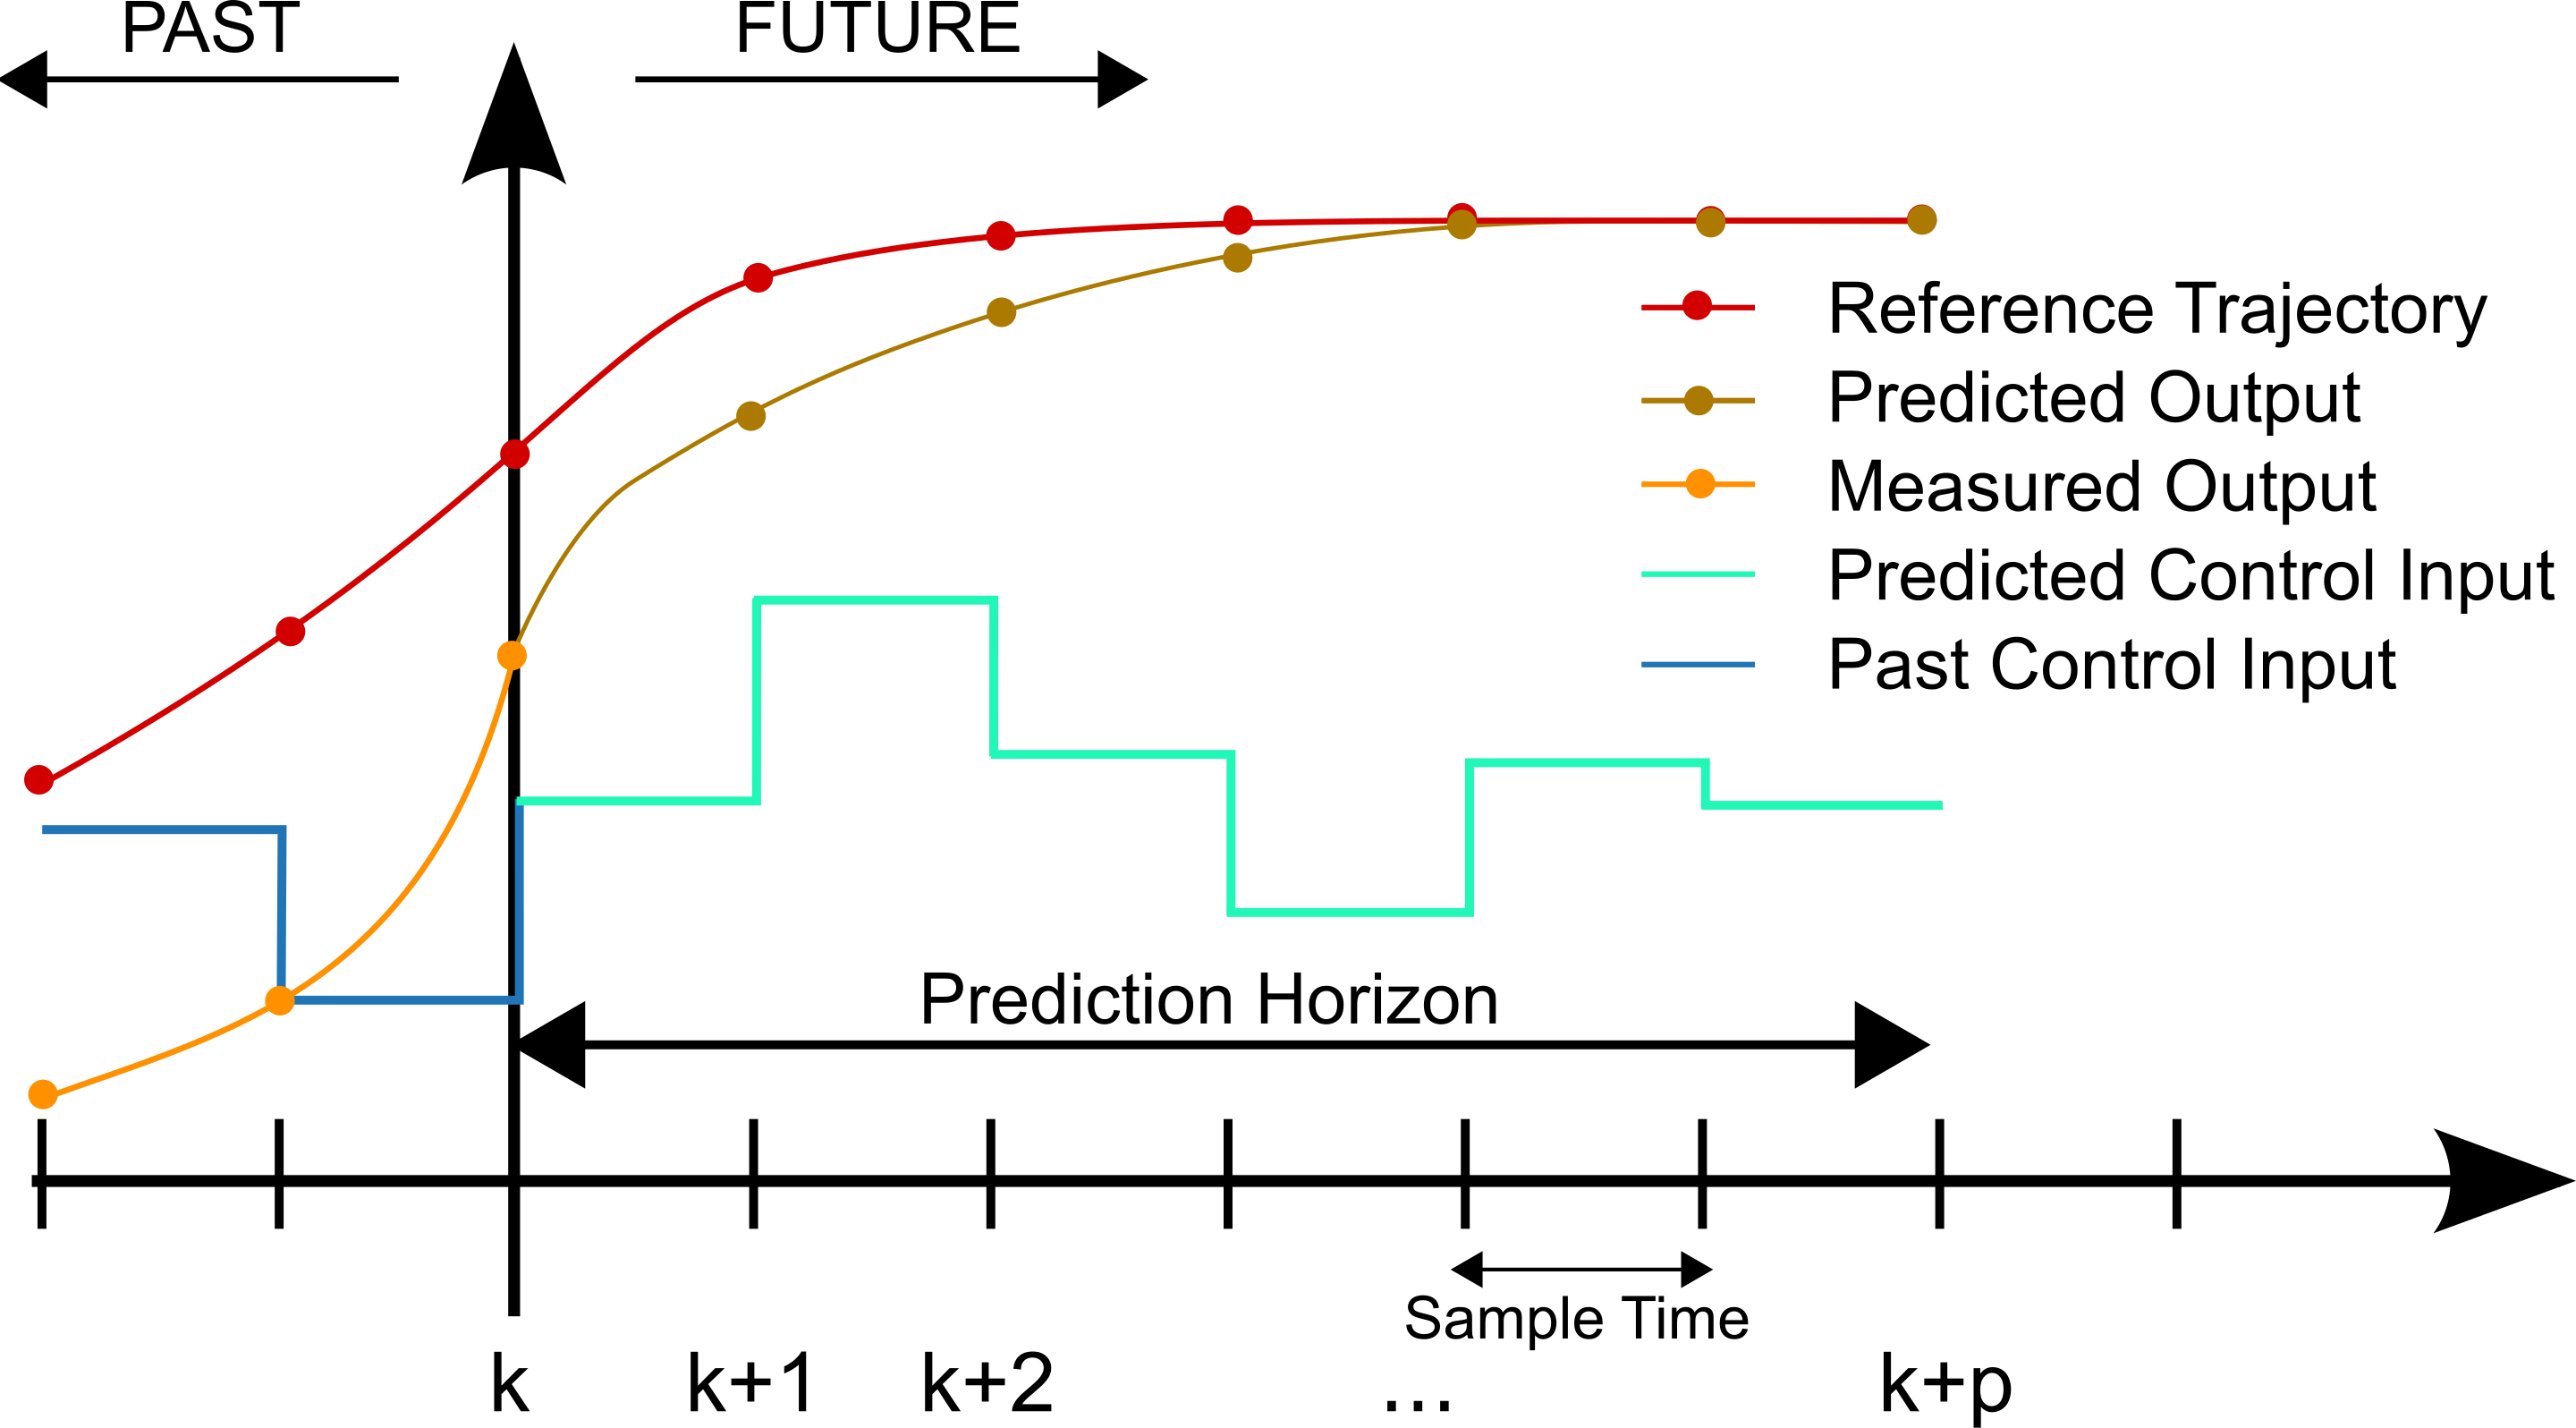
\includegraphics[width=0.8\textwidth]{figures/MPC_scheme_basic.svg.png}
  \caption{Verständnisschema der MPC-Regelung}
  \label{fig:mpc_scheme_basic}
\end{figure}

Beim selbstbalancierenden Fahrrad besteht das Fahrtrichtungsproblem darin, aus Kamerainformationen einen Sollkurs abzuleiten und das Fahrzeug 
mit begrenztem Lenkradius und Lenkrate entlang dieser Trajektorie zu führen.  Der in der Vision‑Regelung verwendete \texttt{VisionMPCController} 
modelliert das Fahrzeug als einfaches Fahrraddynamikmodell mit Zustandsvektor \(x=[x, y, v,\psi]\) für Position, Geschwindigkeit und Gierwinkel 
sowie Eingangsvektor \(u=[a,\delta]\) für Beschleunigung und Lenkwinkel.  Aus dem aktuellen Zustand und dem lateral 
gemessenen Fehler wird ein Referenzpfad erzeugt (Ziel‑Yaw proportional zum Fehler), der über einen Horizont \(T\) vorwärts projiziert wird.  
Anschließend löst der MPC ein konvexes Optimierungsproblem, das die Abweichung von diesem Pfad, die Eingangsgrößen sowie deren zeitliche 
Änderung in einer quadratischen Kostenfunktion gewichtet und durch Beschränkungen auf maximalen Lenkwinkel, Lenkrate, Geschwindigkeitsbereich 
und Beschleunigung ergänzt.  Stehen geeignete Optimierungslöser (z.\,B. \texttt{cvxpy}) zur Verfügung, werden aus diesem Problem kontinuierliche 
Stellgrößen \(\delta\in[-\delta_{\max},\delta_{\max}]\) berechnet, andernfalls fällt der Controller auf eine einfache P‑Regelung zurück.  
Vor der Weitergabe an den schnellen Balance‑Controller werden die resultierenden Lenkwinkel und Beschleunigungen normiert, geglättet und auf Änderungsraten 
begrenzt, um ruckfreie Übergänge zu gewährleisten \cite{vision_mpc_readme}. Eine spezifische erklärung der implementierten Regelung findet sich in Kapitel 5.2.

Die Eignung der MPC Regelung für das Fahrtrichtungsproblem ergibt sich aus der Vorhersagefähigkeit und der Einbeziehung von Beschränkungen.  
Das Fahrradsystem ist nichtlinear und um einer gekrümmten Spur zu folgen, muss der Regler zukünftige Kurvenverläufe 
berücksichtigen und gleichzeitig mechanische Limits (Lenkeinschlag, Lenkrate) respektieren.  MPC kann diese Randbedingungen explizit 
in das Optimierungsproblem integrieren und die Stellgrößen so wählen, dass sowohl die Trajektorienabweichung als auch der Stellaufwand 
minimiert werden.  In Yasin Girays Masterarbeit wurde der visionbasierte MPC‑Regler mit einem Horizont von \(T=3\) und den genannten 
Zuständen und Eingängen implementiert und mit Gewichten auf Zustände, Eingänge und deren Differenzen parametriert.  
Simulationen zeigten, dass das Fahrrad mithilfe des MPC gleichmäßig entlang der aus der Bildsegmentierung abgeleiteten Spur navigierte und 
dabei die mechanischen Limits einhielt.  Somit stellt MPC einen geeigneten Ansatz dar, um das autonome Fahrrad stabil und vorausschauend 
entlang einer vorgegebenen Fahrtrichtung zu steuern.

\subsection{YOLO-Grundlagen und Segmentierung} \label{chap:yolo}

You Only Look Once (YOLO) ist eine Reihe von Echtzeit‑Objekterkennungsverfahren, die auf Convolutional Neural Networks basieren.  Das ursprüngliche YOLO wurde 
2015 von Redmon et al. vorgestellt und erfordert im Gegensatz zu region‑proposal‑basierten Ansätzen nur einen Vorwärtsdurchlauf durch das Netz, um Klassen und 
Bounding Boxes für alle Objekte in einem Bild bestimmen \cite{yolo_wikipedia}.  Neuere Modelle wie YOLOv8 erweitern die ursprüngliche YOLO-Architektur. 
Sie können nicht nur Objekte erkennen, sondern auch Bilder klassifizieren und Instanzen segmentieren. Ein moderner, leichter Backbone
\footnote{Der Backbone ist das Merkmalsextraktionsnetz der Architektur. Er transformiert das Eingabebild in hierarchische, mehrskalige 
Feature-Maps, die die Grundlage für Klassifikation, Lokalisierung und Segmentierung bilden.}, ein ankerfreier 
Detektionskopf \footnote{Ankerfrei bedeutet ohne vordefinierte Ankerboxen. Der Kopf schätzt pro Bildposition direkt Objektzentren und 
Boxparameter sowie Klassenwahrscheinlichkeiten, was Hyperparameter reduziert und das Matching im Training vereinfacht.} und verbesserte 
Verlustfunktionen erhöhen Effizienz und Genauigkeit. Dadurch laufen die Modelle auf vielen Hardwareplattformen zuverlässig und schnell \cite{openmmlab_yolov8}.

Bei der Bildsegmentierung wird jedem Pixel eines Bildes ein Label zugeordnet.  Semantic Segmentation ordnet jedem Pixel eine Objektklasse zu, ohne zwischen 
einzelnen Instanzen zu unterscheiden, während Instance Segmentation jedes Pixel einer individuellen Objektinstanz zuordnet \cite{image_segmentation_wikipedia}.  
Panoptic Segmentation kombiniert beide Ansätze, indem sie sowohl die Klasse als auch die Instanz für jedes Pixel identifiziert \cite{image_segmentation_wikipedia}. 
 In der Instanzsegmentierung liefert das Netzwerk neben Bounding Boxes auch Masken, die die Form jedes erkannten Objekts abbilden.

 YOLOv8 erweitert die Objekterkennung um Instanzsegmentierung, wobei ein auf YOLACT \footnote{YOLACT steht für You Only Look At Coefficients 
 und ist ein einstufiges Verfahren zur Instanzsegmentierung. Es erzeugt Prototypmasken und kombiniert sie mit Koeffizienten zu Objektmasken} 
 basierender Kopf für jedes erkannte Objekt eine zusätzliche Maske berechnet \cite{openmmlab_yolov8}.  
 Durch diese Erweiterung kann ein Modell in einem einzigen Forward‑Pass sowohl Objekte lokalisieren als auch 
deren pixelgenauen Umrisse bestimmen.  Wie bei früheren YOLO‑Versionen werden Varianten unterschiedlicher Größe bereitgestellt (Nano, Small, Medium, Large usw.), 
um den Kompromiss zwischen Geschwindigkeit und Genauigkeit zu steuern \cite{openmmlab_yolov8}.

In dieser Arbeit wird eine YOLOv8‑basierte Segmentierung für die Umfeldwahrnehmung genutzt.  Das Modell ist auf vier Klassen trainiert: Wiese 
(„meadow“), Hindernis („obstacle“), Hauptfahrbahn („street\_main“) und Seitenfahrbahn („street\_side“), wie in Abbildung \ref{fig:yolo} zu sehen ist \cite{vision_mpc_readme}. Dabei liefert es
pro Klasse ein Pixelmasken Overlay sowie die zugehörigen Bounding Boxes.  Anschließend wird aus dem Segment „street\_main“ der laterale Fehler 
bestimmt, der als Eingang für die Pfadverfolgung dient.  Die genauen Details zur Modellauswahl, Datensatzgenerierung und Implementierung werden 
in einem späteren Kapitel beschrieben.  Hier soll lediglich hervorgehoben werden, dass die Kombination aus schneller YOLO‑Detektion und Instanzsegmentierung 
eine effiziente und genaue Grundlage für die kamerabasierte Fahrspurerkennung bildet.





\begin{figure}[H]
  \centering
  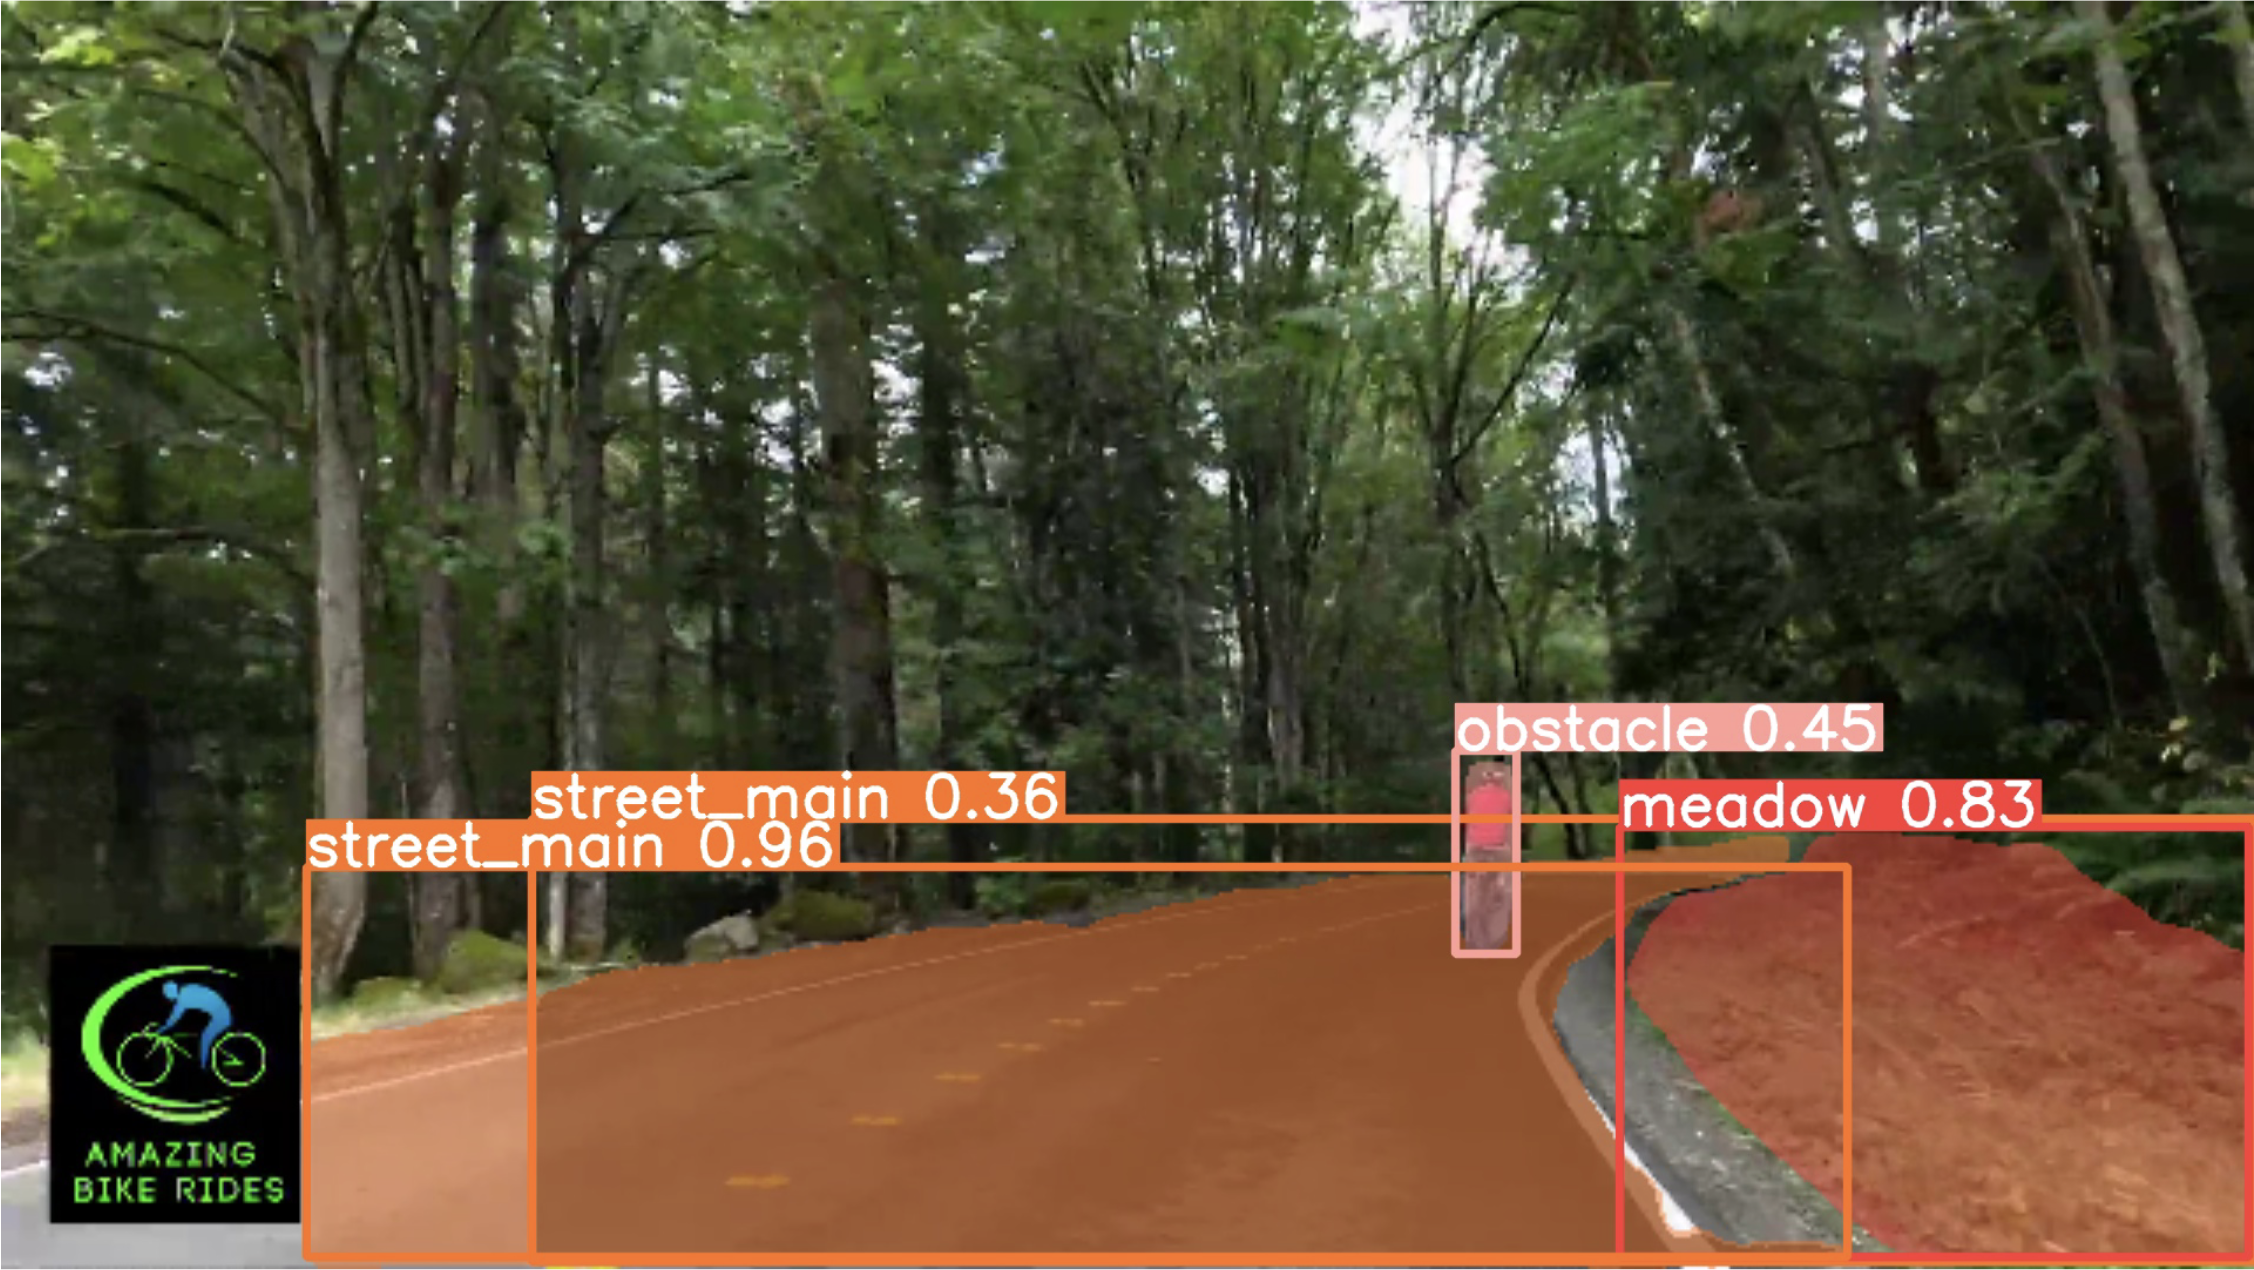
\includegraphics[width=0.8\textwidth]{figures/Yolo.png}
  \caption{YOLO-Segmentierung mit YOLOv8}
  \label{fig:yolo}
\end{figure}
%--------------------------------------------------
% Webots-Simulationsumgebung
%--------------------------------------------------
  
\newpage
\section{Webots-Simulationsumgebung}
  Hier wird die in Webots realisierte Simulationsumgebung vorgestellt, die als zentraler Versuchsstand für Entwurf, Parametrierung
  und Evaluation der kombinierten Regelung des selbstbalancierenden Fahrrads dient. Ziel ist es, ein reproduzierbares und sicheres  
  Testbett zu schaffen, in dem das physikalische Fahrverhalten, die sensorgeführte Pfadverfolgung sowie die Kopplung von schneller
  Balance-Regelung und langsamer Vision-/Trajektorienplanung unter kontrollierten Bedingungen untersucht werden können. Webots
  bietet dafür eine deterministische Dynamiksimulation auf Basis von ODE, eine hierarchische Szenenbeschreibung und eine klare
  Trennung von Geometrie, Physik, Sensorik, Aktuatorik und Controllern – Eigenschaften, die systematische Parameterstudien,
  Logging und automatisierte Auswertung wesentlich erleichtern \cite{cyberbotics2025}.

  Das Kapitel ist wie folgt strukturiert: Zunächst wird ein Überblick über Webots und die genutzten Kernfunktionen gegeben.
  Anschließend wird die konkrete Szenenstruktur der Weltdatei erläutert, einschließlich globaler Simulationsparameter und
  der Organisation der Knoten. Darauf aufbauend folgt die Beschreibung des Fahrradmodells mit seinen Gelenken, Kontakt- und
  Masseneigenschaften sowie der eingesetzten Sensoren und Aktuatoren. Abschließend werden die Controller-Prozesse und deren
  Interaktion skizziert sowie die angebundene GUI bzw. Auswertepfade beschrieben. Diese Gliederung macht transparent, wie
  ausgehend von einem konsistenten physikalischen Modell die Regelungsalgorithmen iterativ entwickelt, validiert und
  für den späteren Transfer auf den Realprototyp vorbereitet werden.



  \subsection{Überblick}
  Webots ist ein frei verfügbares, quelloffenes und plattformunabhängiges Robotik Simulationsprogramm, das seit 1998 kontinuierlich 
  gepflegt wird und in Forschung, Lehre und Industrie breite Anwendung findet \cite{michel2004,cyberbotics2025}. Es kombiniert eine 
  moderne Qt\-Benutzeroberfläche mit einer Mehrkörper\-Dynamiksimulation auf Basis der \emph{Open Dynamics Engine} (ODE) sowie einer 
  OpenGL\-gestützten Rendering\-Pipeline. Dadurch lassen sich fotorealistische 3D\-Szenen mit deterministischem Integrationsschema und 
  feingranularer Kontrolle der Simulationszeit schrittgenau ausführen \cite{cyberbotics2025}.

  Kern des Webots\-Modells ist die hierarchische Szenenrepräsentation in \textit{World}\-Dateien 
  (\texttt{*.wbt}; VRML\-basiert). 
  Eine Welt kapselt globale Parameter (z.\,B.\ Zeitauflösung, Kontakt\- und Reibungsmodelle), Umgebungsobjekte (Boden, Licht, Hintergrund) 
  sowie Roboterknoten mit Sensorik, Aktuatorik und Masseneigenschaften. Geräte (z.\,B.\ Kamera, IMU, Lidar, \texttt{RotationalMotor}) 
  sind als Nodes mit klar definierten Schnittstellen realisiert; ihre Parameter (Auflösung, Bildfrequenz, Dämpfung, Grenzwerte) sind 
  reproduzierbar konfigurierbar. Controller laufen als getrennte Prozesse in C/C++, Python, Java oder MATLAB und kommunizieren zur Laufzeit 
  über wohldefinierte APIs mit der Simulationswelt; mittels ROS~2\-Bridge ist zudem eine Einbettung in verteilte Robotik\-Stacks möglich 
  \cite{gupta2023,cyberbotics2025}. Eine spezielle \emph{Supervisor}\-API erlaubt höherwertige Eingriffe (Positionsreset, automatisiertes 
  Logging, Metrik\-Auswertung) und bildet die Grundlage für reproduzierbare Benchmarking\-Pipelines \cite{cyberbotics2025}.

  Für regelungsorientierte Studien bietet Webots drei Eigenschaften, die in dieser Arbeit zentral sind: (i) \emph{Determinismus} durch festen 
  Zeitschritt und explizite Integrationsreihenfolge, was faire Parameterstudien ermöglicht; (ii) \emph{Modularität} durch die Trennung von 
  Geometrie, Physik, Sensorik/Aktuatorik und Controllern, wodurch Varianten (z.\,B.\ Reibungskoeffizienten, Trägheiten, Abtastraten) isoliert 
  untersucht werden können; (iii) \emph{Automatisierbarkeit} über den Supervisor, u.\,a.\ für Szenario\-Resets, Störgrößeninjizierung, Batch\-Runs 
  und standardisierte Ergebnisberichte \cite{cyberbotics2025}.

  Relevanz für \emph{fahrdynamische Einspurfahrzeuge}: In jüngeren Arbeiten wird Webots gezielt zur Simulation von Fahrrädern und Motorrädern 
  eingesetzt. Das Open\-Source\-Add\-on \emph{WeBikes} erweitert Webots um ein konfigurierbares, physikalisch fundiertes Einspurfahrzeugmodell 
  (Geometrie, Masseverteilung, Reifenkontakt, Steuerkinematik) und demonstriert, dass typische Phänomene wie Selbststabilisierung, Lenkdynamik 
  und Kurvenfahrt reproduzierbar abgebildet werden können \cite{li2024webikes}. Damit wird ein freier, reproduzierbarer Vergleich zu Spezialwerkzeugen 
  ermöglicht und eine Brücke zwischen Regelungsentwurf (z.\,B.\ Balanceregelung, MPC\-Trajektorienplanung) und virtuellen Fahrversuchen geschlagen. 
  Über den gleichen Mechanismus nutzen weitere Studien Webots als Digital\-Twin\-Plattform für komplexe, materialabhängige Systeme (z.\,B.\ weiche Greifer),
   was die Übertragbarkeit auf neuartige Robotertypen unterstreicht \cite{hadi2024softgripper}.

  Für diese Arbeit ist Webots folglich ein geeignetes Testbett, um die Kopplung einer schnellen Balance\-Regelung (PID, \(\approx\)kHz\-Skala) mit einer 
  langsameren vision\- bzw.\ modellprädiktiven Pfadführung (tens of Hz) systematisch zu entwerfen, zu parametrieren und zu evaluieren. Die klare Trennung 
  der Subsysteme (Physik, Sensorik, Controller) erlaubt ablation\-artige Studien (z.\,B.\ Variation von Zeitschritt/Reibung, Sensorausfall, Verzögerungen), 
  während die Supervisor\-Schnittstelle reproduzierbare Kampagnen mit konsistentem Logging unterstützt \cite{cyberbotics2025}.




  \subsection{Struktur der Simulationsumgebung}
  Die verwendete Simulationsumgebung basiert auf Webots und damit auf einer hierarchisch organisierten Szenenbeschreibung 
  im VRML-Format. Eine \texttt{.wbt}-Datei kapselt sämtliche Entitäten der virtuellen Welt – von globalen 
  Parametern (Zeitauflösung, Kontaktmodelle) über Umgebungsobjekte (Boden, Hintergrund, Lichtquellen) bis 
  hin zu Robotern mitsamt deren Sensorik, Aktuatorik und Controllern \cite{cyberbotics2025,gupta2023}. Jeder Knoten (Node) kann wiederum 
  Unterknoten besitzen, sodass sich komplexe Systeme modular aus standardisierten Bausteinen zusammensetzen 
  lassen. Für die vorliegende Arbeit ist diese Hierarchie entscheidend, weil sie erlaubt, (i) das physikalische 
  Verhalten des Fahrrads getrennt von (ii) der Szenengeometrie und (iii) den übergeordneten Reglerprozessen 
  zu modellieren. Änderungen an einem Teilbereich – etwa an den Reibungsparametern der Reifen oder an der 
  Position einer Kamera – bleiben somit lokal und beeinträchtigen die übrigen Komponenten nicht.
  
  Ausgangspunkt der Welt ist eine rechteckige Bodenarena mit texturierter Fahrbahnoberfläche, die als Referenzstrecke 
  für die visuelle Spurführung dient. Globale Kontakt- und Reibungsparameter sind hier definiert, um das Zusammenspiel 
  zwischen Reifen und Untergrund konsistent zu halten. Ein fester Zeitschritt im Millisekundenbereich stellt sicher, 
  dass sowohl die Balancebewegungen des Fahrrads als auch die Bildverarbeitungsschleifen deterministisch und in Echtzeit 
  simuliert werden können \cite{cyberbotics2025}. Die Kameraperspektive des Betrachters (Viewpoint) folgt dem Fahrrad aus erhöhter Position, 
  was die visuelle Analyse der Fahrmanöver während der Versuche erleichtert.
  
  Das zentrale Element der Szene ist der Roboterknoten \emph{BICYCLE}, der das selbstbalancierende Fahrrad repräsentiert. 
  Sein Geometriemodell wurde aus CAD-Daten übernommen und mit vereinfachten Kollisionsvolumina (Boxen und Zylinder) hinterlegt, 
  um die Physiksimulation effizient zu halten. Die Massen- und Trägheitsparameter der Baugruppen (Rahmen, Räder, Gabel) sind 
  explizit angegeben, sodass die Dynamik – insbesondere Roll- und Nickbewegungen – realitätsnah nachgebildet wird. Bewegliche 
  Komponenten sind über Hinge-Joints angebunden: Das Hinterrad wird über einen Rotationsmotor für den Vortrieb angesteuert, 
  die Lenkbewegung des Vorderrads erfolgt über ein zweites Gelenk mit eigenem Servomotor. Ergänzend existiert ein Kurbel-/Pedal-Gelenk, 
  das in erster Linie der geometrischen Vollständigkeit und nicht der Antriebserzeugung dient. Zur Zustandserfassung sind 
  Sensorschnittstellen integriert: Eine Inertialmesseinheit (IMU) liefert dem Balance-Regler fortlaufend Orientierung und 
  Rollwinkel \cite{bno055}; eine am Fahrrad montierte Kamera kann genutzt werden, um on-board visuelle Informationen 
  auszuwerten. Ein Display-Modul steht optional für Debug- oder Visualisierungszwecke zur Verfügung. Die Kommunikation 
  zwischen Fahrrad und übergeordnetem Regler erfolgt über ein Paar aus \texttt{Emitter} und \texttt{Receiver}, die einen 
  leichten, paketbasierten Nachrichtenaustausch innerhalb von Webots ermöglichen.
  
  Übergeordnet ist ein \emph{Supervisor}-Knoten angelegt. Dieser spezielle Robotertyp besitzt in Webots weitreichende 
  Eingriffsmöglichkeiten auf Welt-Ebene (z.\,B. Position-Reset, Logging, automatisierte Auswertung) und dient hier als 
  externe Beobachter- und Steuerinstanz. Der Supervisor trägt eine statisch in der Szene platzierte Kamera, die die Fahrbahn 
  aus einer globalen Perspektive erfasst. Auf Basis dieser Bilder führt der Python-basierte Vision-Controller eine 
  Spurdetektion (YOLO) durch und berechnet über ein modellprädiktives Regelungsverfahren (MPC) Lenksollwerte bzw.\ Trajektorien. 
  Diese Kommandos werden per Funkkanal (Emitter) an den Balance-Controller des Fahrrads übertragen, der sie in konkrete 
  Motorbefehle umsetzt. Umgekehrt sendet das Fahrrad Statusdaten zurück, die der Supervisor für Evaluations- und Loggingzwecke 
  speichert. Dieses Zusammenspiel zweier Controller-Prozesse – ein echtzeitnaher PID-Regler in C auf Roboterseite und ein 
  bildverarbeitungsgetriebener MPC-Regler in Python auf Supervisorebene – bildet die Kernstruktur der kombinierten Regelung.
  
  Die gewählte Struktur der Simulationsumgebung verfolgt zwei Ziele: Erstens ermöglicht sie reproduzierbare und sichere 
  Experimente in verschiedensten Fahrszenarien (Geradeausfahrt mit Störimpuls, Slalomkurse, Kurvenfahrten mit Steigung), 
  ohne das reale Hardware-Risiko des Umkippens oder der Beschädigung einzugehen. Zweitens gestattet die klare Trennung von 
  physikalischem Modell, Sensorebene und Reglerlogik eine gezielte Variation einzelner Parameter (z.\,B. Reibung, Zeitschritt, 
  Bildauflösung), um deren Einfluss auf die Gesamtperformance systematisch zu untersuchen. Webots fungiert damit als flexibles 
  Testbett, in dem sowohl Balance- als auch Spurführungsalgorithmen iterativ entwickelt, validiert und optimiert werden können, 
  bevor sie auf den realen Prototyp übertragen werden.
  \pdfcomment{Bild der Struktur der Simulationsumgebung anzeigens}





  \newpage



  \subsection{Das Fahrradmodell}
  \begin{wrapfigure}{r}{0.42\textwidth} % r=rechts, l=links
    \vspace{-0.8\baselineskip}          % optional: nach Bedarf anpassen
    \centering
    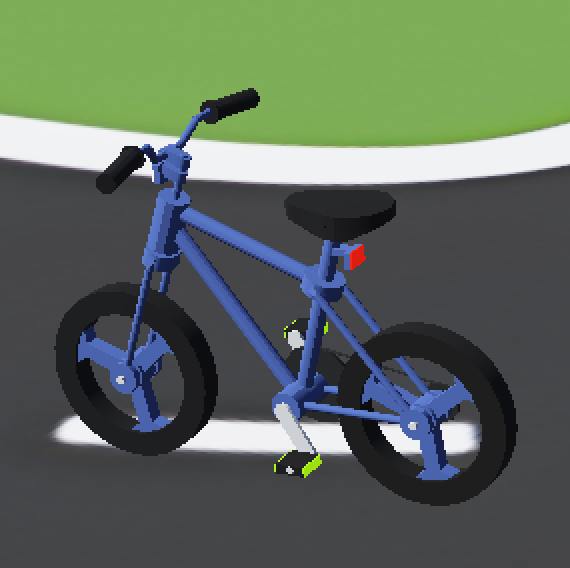
\includegraphics[width=\linewidth]{figures/bicycle.png}
    \caption{Das Fahrradmodell in Webots.}
    \label{fig:bicycle}
  \end{wrapfigure}

  Das folgende Kapitel führt in das in Webots implementierte Fahrradmodell ein, 
  wie es in der \texttt{.wbt}-Datei spezifiziert ist. 
  Das Modell ist als kinematischer Baum aus starren Körpern (\texttt{Solid}) aufgebaut, die über eindimensionale Drehgelenke 
  (\texttt{HingeJoint}) verbunden sind. Die sichtbare Geometrie (\texttt{CadShape}) ist vom physikrelevanten Kollisionsmodell 
  (\texttt{boundingObject} mit einfachen Primitiven) getrennt; Masse, Schwerpunkt und Trägheit sind im \texttt{Physics}-Block definiert. 
  An ausgewählten Gelenken wirken \texttt{RotationalMotor}-Aktuatoren, während Dämpfung und Haftreibung über 
  \texttt{HingeJointParameters} festgelegt sind. In den nachfolgenden Unterabschnitten werden die Baugruppen des Fahrrads entlang 
  der Knotenstruktur der Weltdatei beschrieben und deren Parameter hinsichtlich ihres Einflusses auf die Dynamik (Lenkung, 
  Rad–Boden-Kontakt, Eigendämpfung) erläutert.

  %\subsubsection{Hinterrad (\texttt{DEF rear\_wheel})}
  Der Knoten \texttt{rear\_wheel} ist Teil des Gesamtfahrrads und definiert das angetriebene Hinterrad (\texttt{HingeJoint}).
  Die \texttt{HingeJointParameters} beschreiben das Lager des Hinterrads. Der \emph{anchor} \verb|0 0.5312 0| gibt die Position 
  der Radachse im Elternkoordinatensystem an. Die \emph{dampingConstant} \verb|0.8| ist die viskose Dämpfung des Lagers: höher 
  bedeutet mehr Beruhigung gegen Schwingungen, aber eine trägere Rotation. Die \emph{staticFriction} \verb|0.1| ist die Haftreibung 
  im Lager: sie verhindert kleines Flattern nahe Stillstand, erhöht jedoch das zum Anfahren nötige Drehmoment.
  Das \texttt{endPoint Solid} ist der vom Gelenk bewegte starre Körper auf der Kind-Seite des \texttt{HingeJoint}. 
  Er rotiert um den am Gelenk definierten Anker/Achse und bildet damit das eigentliche Bauteil (hier: das Hinterrad), 
  das durch die Bewegung betroffen ist. In der Hierarchie gilt: Elternteil → Gelenk → \texttt{endPoint Solid}; alles, was hier angehängt ist, bewegt sich mit.
  Das \texttt{boundingObject} definiert die kollisions- und kontaktrelevante Geometrie des Hinterrads, unabhängig vom sichtbaren Mesh. 
  Es bestimmt, wo das Rad den Boden „berührt“, wo Kräfte eingeleitet werden und wie Kollisionen erkannt werden. Im Modell ist es ein einfacher Zylinder, 
  der per \texttt{Pose}-Rotation (entspricht Drehung um die \(y\)-Achse um \(90^\circ\)) in die Radebene gedreht wird; so bildet er die Kontaktfläche des Reifens ab. Zusammen mit dem 
  \texttt{contactMaterial} (z.\,B.\ \texttt{"wheel"}) entstehen daraus die Reib- und Rückpralleigenschaften im Kontakt mit dem Untergrund. 
  Größe und Ausrichtung des \texttt{boundingObject} sollten zur realen Radgeometrie passen, da es die Kontaktlage und damit das 
  Fahrverhalten maßgeblich beeinflusst.
  \paragraph{Physik (\texttt{Physics})}
  Der \texttt{Physics}-Block definiert die Masseneigenschaften des Hinterrads. \texttt{density -1} bedeutet: Masse und Trägheit werden 
  \emph{nicht} aus dem \texttt{boundingObject} berechnet, sondern mit \texttt{mass}, \texttt{centerOfMass} und \texttt{inertiaMatrix} 
  explizit vorgegeben. \texttt{mass 2} setzt die Gesamtmasse (kg), \texttt{centerOfMass [0 0 0]} positioniert den Schwerpunkt im Solid-Frame (hier an der Nabe), 
  und \texttt{inertiaMatrix [0.122 0.122 0.245 0 0 0]} legt die Rotations-Trägheiten (kg·m\(^2\)) fest; größere Werte bedeuten trägere Reaktion auf 
  Dreh- bzw.\ Kippbewegungen. Die Off-Diagonale \verb|0 0 0| zeigt an, dass Hauptachsen und Solid-Achsen ausgerichtet sind. Für automatische Berechnung 
  könnte statt \verb|density -1| eine positive Dichte verwendet werden (dann kommen Masse/Trägheit aus Volumen×Dichte des \texttt{boundingObject}).



  \begin{lstlisting}[style=wbt,caption={Hinterrad—Kinematik, Kontakt und Physik (Auszug)},label={lst:rear_wheel}]
  DEF rear_wheel HingeJoint {
    jointParameters HingeJointParameters {
      anchor 0 0.5312 0
      dampingConstant 0.1
      staticFriction 0.8
    }
    device [..] # RotationalMotor (siehe Kaptitel 4.5 Aktuatoren)
    endPoint Solid {
      children [
        Transform {...}  # visuelles Mesh (ohne Physik)
      ]
      contactMaterial "wheel"
      boundingObject Pose {
        rotation 0 1 0 1.5708
        children [ Cylinder { height 0.05  radius 0.352  subdivision 72 } ]
      }
      physics Physics {
        density -1, mass 2, centerOfMass [ 0 0 0 ], 
        inertiaMatrix [ 0.122  0.122  0.245   0 0 0 ]
      }
    }
  }
  \end{lstlisting}




  \subsection{Sensoren}
  Für die Stabilisierung und Spurführung des selbstbalancierenden Webots-Fahrrads 
  kommen mehrere Sensorsysteme zum Einsatz. Zentral sind eine \textbf{Inertialmesseinheit}
  (IMU) am Fahrzeug zur Lageerfassung und eine \textbf{Kamera} zur optischen Fahrwegdetektion. Ergänzend liefern \textbf{Motorsensoren} (Encoder) an den Achsen Messgrößen wie Lenk- und 
  Raddrehwinkel. Die IMU versorgt den inneren schnellen Regelkreis (Balance-PID) laufend mit dem aktuellen Rollwinkel, während die Kamera den äußeren, langsamer 
  abtastenden Regelkreis (vision-basiertes MPC) mit Spurabweichungsinformationen speist. Beide Sensorströme werden anschließend in einfacher Weise fusioniert, um 
  die Regelgrößen an die Aktuatoren (Lenkmotor und Antrieb) auszugeben GitHubGitHub . Im Folgenden werden die einzelnen Sensoren hinsichtlich physikalischer Funktion, 
  Modellierung in Webots, Rolle im Regelkreis und Integration im Quellcode beschrieben.
  
  %--------------------------------------------------
  % Inertialmesseinheit (IMU)
  %--------------------------------------------------
  
  \subsubsection{Inertialmesseinheit (IMU)}

  \textbf{Physikalisches Prinzip:} Eine Inertial Measurement Unit (IMU) erfasst Trägheitsgrößen des Fahrzeugs, typischerweise mit kombinierter \textbf{Beschleunigungsmessung} (Accelerometer) und 
  \newline\textbf{Drehratensensoren} (Gyroskope) auf drei Raumachsen \cite{cyberbotics_inertialunit}. Durch Fusion dieser Signale – oft ergänzt um einen Magnetometer-Kompass – 
  lässt sich die Orientierung im Raum bestimmen. Im realen Prototyp kommt z.\,B. der IMU-Sensor \textbf{BNO055} zum Einsatz, der intern die Rohdaten filtert und direkt \textbf{Euler-Winkel} 
  (Roll, Pitch, Yaw) bereitstellt \cite{bno055}. Die Rollachse (Seitenneigung) ist beim Fahrrad die entscheidende Stabilitätsgröße.  Reale IMUs liefern diese Winkel mit begrenzter Auflösung 
  und unterliegen Rauschen sowie Drift, was meist durch Kalibrierung und Sensorfusion 
  kompensiert werden muss. Die Ausgaberate moderner IMUs liegt im Bereich mehrerer hundert Hertz (der BNO055 etwa $\sim$200~Hz \cite{bno055}), 
  was für eine schnelle Lagekontrolle ausreicht.

  \textbf{IMU-Modell in Webots:} Webots stellt mit dem \texttt{InertialUnit}-Knoten ein abstraktes IMU-Modell bereit, das idealisierte Orientierungsdaten liefert. Konkret berechnet und 
  aktualisiert das InertialUnit-Gerät in jeder Simulationsschleife den \textbf{Kipp- und Gierwinkel} des Roboters relativ zu einem globalen Bezugssystem \cite{cyberbotics_inertialunit}. 
  Im Gegensatz zu einer realen IMU entfallen hier Kalibrierfehler und Rauschen – die Simulation liefert die Orientierungswinkel also praktisch \textbf{fehlerfrei und ohne Drift}. 
  Das im Webots-Weltmodell definierte Gerät \texttt{imu} ist starr im Fahrradrahmen verbaut (an geeigneter Position, etwa nahe dem Schwerpunkt) und gibt standardmäßig 
  Roll-, Pitch- und Yaw-Winkel in Radiant aus. Die Abtastung erfolgt synchron mit dem physikalischen Simulationszeitschritt. Im vorliegenden Modell ist der \texttt{basicTimeStep} 
  der Welt auf 2~ms gesetzt \cite{githubWebots}, was einer Messfrequenz von 500~Hz entspricht. Dadurch  können selbst schnelle Kippbewegungen des Fahrrads in Echtzeit erfasst werden \cite{githubWebots}.

  \begin{figure}[h]
    \centering
    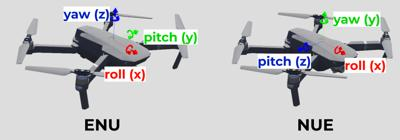
\includegraphics[width=0.8\textwidth]{figures/enu_nue.thumbnail.jpg}
    \caption{IMU-Knoten in Webots.}
    \label{fig:imu}
  \end{figure}
  
  \textbf{Rolle im Regelkreis:} Der IMU-Sensor bildet die zentrale \textbf{Rückführung} für die 
  \textbf{Balance-Regelung}. In jedem Simulationsschritt liest der PID-Regler 
  den aktuellen Rollwinkel $\varphi_{\text{roll}}$ aus der IMU und berechnet daraus 
  die Stellgröße für den Lenkantrieb. Konkret fungiert der Rollwinkel als 
  \emph{Regelgröße} im inneren Regelkreis: weicht das Fahrrad nach links/rechts ab, 
  soll durch einen entsprechenden Lenkeinschlag gegengesteuert werden, 
  bis $\varphi_{\text{roll}} = 0$ (senkrechte Lage) erreicht ist. Die hohe Abtastrate der IMU erlaubt es, den 
  \textbf{Regelkreis mit einer Zykluszeit von 2 ms} praktisch verzögerungsfrei zu schließen. 
  Dadurch reagiert der PID-Regler sehr schnell auf Lageänderungen, was eine Grundvoraussetzung ist, 
  um das instabile überhaupt beherrschen zu können. Im äußeren (vision-basierten) 
  Regelkreis spielt die IMU direkt keine Rolle, allerdings fließen die Balancierinformationen indirekt ein, wenn die Vision-Steuerung, 
  z.\,B. die Fahrgeschwindigkeit reduziert, sobald der Stabilitätsfaktor sinkt (starke Schräglage detektiert). 
  Insgesamt sorgt die IMU dafür, dass die \textbf{Regelstrecke} mit hoher Güte beobachtet wird, und bildet so das Fundament der Stabilisierung.


  Im C-Controller \texttt{balance\_control.c} wird die IMU über die Webots-API 
  initialisiert und ausgelesen. Listing~1 zeigt auszugsweise, wie das Gerät referenziert, 
  aktiviert und genutzt wird. Zunächst wird der Device-Tag der IMU mit ihrem Namen 
  \texttt{"imu"} angefordert und das Sensor-Sampling mit dem Simulationstimestep 
  (2~ms) eingeschaltet. In der Hauptschleife ruft der Regler dann kontinuierlich die Funktion 
  \texttt{wb\_inertial\_unit\_get\_roll\_pitch\_yaw()} auf, welche einen Vektor der Winkel zurückliefert. 
  Der Rollwinkel (Index 0 des Arrays) wird extrahiert und in die Regelung eingespeist. 
  Da die Webots-IMU per se idealisiert ist, entspricht dieser Winkel exakt der aktuellen 
  Fahrzeugneigung ohne Messfehler. Im Code ist dennoch ein Fallback vorgesehen: Falls der Supervisor-Knoten verfügbar ist, 
  wird alternativ dessen Orientierungs\-matrix ausgewertet – dies diente experimentell 
  der Verifikation der IMU-Daten und kann die gleiche Information liefern. 
  Im Normalfall nutzt der PID jedoch direkt die IMU-Daten. Der exemplarische Code zeigt, wie einfach die Orientierung in Webots abgefragt werden kann, 
  verglichen mit einer realen IMU (wo man per I\textsuperscript{2}C erst Rohdaten lesen und konvertieren müsste). 
  Die geringe Latenz der \texttt{wb\_inertial\_unit\_get\_roll\_pitch\_yaw}-Funktion 
  (nur ein Zeiger auf interne Simulationsdaten) trägt dazu bei, dass der Balance-Regelkreis 
  praktisch ohne zusätzliche Verzögerung arbeitet.


  \begin{lstlisting}[style=wbt,caption={IMU-Initialisierung und -Abfrage im C-Controller (Balance-Regelung)},label={lst:imu}]
    // IMU-Geraet initialisieren (in init_devices)
    imu_sensor = wb_robot_get_device("imu");
    wb_inertial_unit_enable(imu_sensor, timestep);  // Abtastrate = Welt-Zeitschritt (2 ms)
  
    // ... (im Hauptprogramm der Balance-Regelung)
  
    // Roll-, Pitch- und Gierwinkel vom IMU-Sensor abrufen
    const double *rpy = wb_inertial_unit_get_roll_pitch_yaw(imu_sensor);
    double roll_angle = rpy[0];  // aktueller Rollwinkel [Bogenmass]
  \end{lstlisting}
  


  %--------------------------------------------------
  % Kamera
  %--------------------------------------------------
  \subsubsection{Kamera (Videosensor)}

  \textbf{Physikalisches Prinzip:} Die Kamera dient als \textbf{optischer Sensor}, um die Strecke vor dem Fahrrad zu erkennen. Physikalisch basiert 
  sie auf einem \textit{digitalen Bildaufnehmer} (z.\,B. CMOS-Sensor), der durch eine Linse abgebildetes Licht in Pixelwerte umwandelt. In einem 
  realen System würde eine am Fahrzeug montierte Weitwinkel-Kamera laufend \textbf{Videobilder} der Fahrbahn liefern. Wesentliche Parameter sind 
  die \textbf{Auflösung} (Anzahl Pixel, bestimmt Detailgenauigkeit) und die \textbf{Bildrate} (Bilder pro Sekunde, bestimmt zeitliche Auflösung). 
  Für eine stabile Spurhaltung in Echtzeitanwendungen genügen in der Regel zweistellige Bildfrequenzen (\(\sim\!10\text{–}30\,\mathrm{Hz}\)), sofern 
  das Fahrzeug nicht extrem schnell fährt. Die Kamera erfasst visuelle Merkmale der Umgebung – im vorliegenden Kontext insbesondere die 
  \textbf{Straßenmarkierung} bzw. den Verlauf der Fahrspur – die dann von Bildverarbeitungsalgorithmen ausgewertet werden. Physikalisch können \textbf{Umgebungsfaktoren} wie Beleuchtung, 
  Bewegungsunschärfe oder Linsenverzerrungen die Bildqualität beeinflussen, was eine robuste \textbf{Merkmalsextraktion} herausfordernd macht. 
  Im Gegensatz dazu operiert eine Kamera jedoch \textbf{kontaktlos} und kann reichhaltige Umgebungsinformationen liefern, was sie ideal für die 
  \textbf{Pfadführung} macht (im Vergleich zu z.\,B. lokalen Sensorsignalen eines Gyroskops).



  \textbf{Simulation in Webots:} Webots simuliert Kameras über den \texttt{Camera}-Node, der virtuelle Renderings der 3D-Szene erzeugt. 
  Im \textit{Weltfile} ist für den Supervisor (die übergeordnete Instanz) eine Kamera mit definierter Position, 
  Ausrichtung und Eigenschaften eingebettet. Diese sogenannte \textit{Vision-Kamera} blickt aus erhöhter Perspektive 
  nach vorne unten auf die Fahrbahn (vergleichbar mit einer Helm- oder Drohnenkamera, die dem Fahrrad folgt).
  Die in der Simulation gewählte Auflösung beträgt z.\,B. 640$\times$360 Pixel bei einem Gesichtsfeld von ca. 
  114$^{\circ}$ (Field of View $\approx 2.0\,\mathrm{rad}$). Diese Einstellungen sind ein Kompromiss zwischen 
  Sichtfeld und Bilddetail – ein breites Sichtfeld erfasst die S-Kurve vollständig, während die moderate 
  Auflösung die Datenmenge und Rechenzeit begrenzt. Die Kamera liefert pro aktiviertem Zeitschritt ein Bild 
  im \textbf{RGBA-Format} (Rot–Grün–Blau plus Alphakanal) als Array von Byte-Werten.
  In der Controller-Software muss die Kamera explizit aktiviert werden, wobei die Abtastrate frei wählbar ist. 
  Der Vision-Controller nutzt eine Bildrate von rund 20~Hz, entsprechend einem Abtastintervall von 50~ms. 
  Dies ist deutlich langsamer als der Balance-Regelkreis, spiegelt aber die realistische Anforderung wider, 
  dass Bildverarbeitung zeitaufwändiger ist und nicht in jedem Simulationsschritt erfolgen muss. Im Webots-Code wird die Kamera z.\,B. mit 
  \texttt{camera.enable(50)} konfiguriert, sodass alle 50~ms ein neues Frame bereitgestellt wird. 
  Jedes Frame kann vom Controller über \texttt{camera.getImage()} abgeholt und weiterverarbeitet werden. 
  Zu beachten ist, dass Webots standardmäßig keine Kamerarausfälle oder Sensorschwächen simuliert – 
  die gelieferten Bilder sind idealisiert (scharf, bei gleichbleibender Beleuchtung). 
  Um Realismus zu erhöhen, könnten optional Rauschen oder Unschärfe simuliert werden; 
  im gegebenen Modell wird jedoch auf eine idealisierte Spurenerkennung abgezielt.

  \begin{figure}[H]
    \centering
    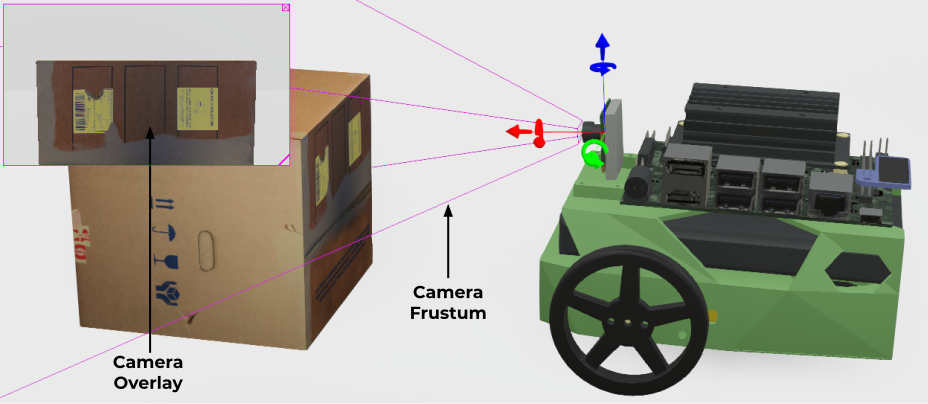
\includegraphics[width=0.8\textwidth]{figures/camera.png}
    \caption{Kamera-Knoten in Webots.}
    \label{fig:camera}
  \end{figure}


  \textbf{Rolle im Regelkreis:} Die Kamera ist der \textbf{Schlüsseleingang} für den vision-basierten äußeren Regelkreis. 
  Ihre Aufgabe besteht darin, dem \textbf{MPC-Fahrtrichtungsregler} Informationen über den Verlauf der Fahrspur 
  relativ zum Fahrzeug zu liefern. Im konkreten Szenario der S-Kurve extrahiert der Vision-Controller aus jedem Kamerabild 
  den lateralen Positionsfehler $e$ der Straße: also wie weit und in welche Richtung 
  das Fahrrad von der gewünschten Spurmitte abweicht. 

  Diese Bildverarbeitung geschieht in mehreren Schritten:


  \begin{enumerate}
    \item \textbf{Merkmalsextraktion:} Zunächst werden relevante Bildmerkmale berechnet, 
    etwa mittels \textbf{Segmentierung} der Straße. 
    Im Projekt wurde hierzu ein vortrainiertes YOLO-Modell verwendet, das die Fahrbahn in der Vogelperspektive segmentiert. 
    Falls kein KI-Modell verfügbar ist, greift ein Fallback auf klassische Bildverarbeitung: 
    Kantenerkennung und Auswertung eines definierten \textit{Region-of-Interest} liefern ebenfalls einen Schätzwert 
    für die Spurmittellage. 
    Ergebnis dieses Schritts ist der Querfehler $e$ (in normierter Form, z.\,B. $-0.5 \dots +0.5$ relativ zur Bildmitte) 
    sowie ggf. zusätzliche Qualitätskennzahlen (etwa die erkannte Kontur oder den Bedeckungsgrad der Fahrbahnmaske).
  
    \item \textbf{Spurführungsregelung:} Auf Basis des visuellen Fehlers bestimmt der Controller 
    einen passenden \textbf{Lenksollwert}. 
    Im entwickelten System kommt hierfür vorzugsweise ein 
    \textbf{modellprädiktiver Regler (MPC)} zum Einsatz, der das Fahrrad als dynamisches Modell 
    (Zustand $\mathbf{x} = [x,y,v,\psi]$) vorausberechnet. 
    Der MPC optimiert die Steuergröße Lenkwinkel $\delta$ (und ggf. Beschleunigung) 
    über einen kurzen Zeithorizont so, dass der Querfehler minimiert und 
    Fahrdynamikgrenzen (Lenkwinkel- und -ratenbegrenzung, Komfort) eingehalten werden. 
  
    Falls der MPC (etwa mangels Rechenpower) nicht verfügbar ist, 
    kann ersatzweise ein einfacherer PID-Ansatz verwendet werden (\textit{„Vision-PID“}), 
    der den Fehler $e$ in einen Lenkwinkel übersetzt. 
    In beiden Fällen resultiert ein Soll-Lenkwinkel $\delta_{\text{sol}}$ 
    bzw. ein normierter Lenkbefehl $u_{\text{vis}} \in [-1,1]$, 
    der an den Balance-Controller gesendet wird. 
  
    Zusätzlich kann die Vision-Einheit eine \textbf{Geschwindigkeitsempfehlung} $v_w$ berechnen – 
    z.\,B. wird bei großem Kurvenfehler eine niedrigere Fahrgeschwindigkeit empfohlen, 
    um die Stabilität zu wahren.
  \end{enumerate}

  \begin{figure}[H]
    \centering
    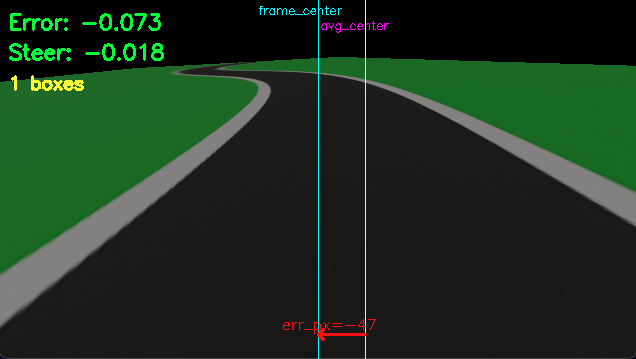
\includegraphics[width=0.8\textwidth]{figures/querfehler.png}
    \caption{Querfehler $e$ der Straße.}
    \label{fig:querfehler}
  \end{figure}

  Die Kamera beeinflusst den Balance-Regler auch indirekt, indem deren Messdaten 
  den \textbf{Kurs der Fahrt} vorgeben. 
  Wichtig ist, dass die Vision-Daten mit deutlich geringerer Frequenz ankommen als die IMU-Daten. 
  Der Balance-Controller hält während der 50~ms zwischen zwei Kamerabildern 
  die zuletzt empfangene Soll-Lenkvorgabe bei und stabilisiert weiterhin autonom. 
  Sobald ein neues Bild ausgewertet ist, wird der Lenksollwert ggf. korrigiert. Dieses \textbf{zweistufige Regelungskonzept} 
  (innere IMU-Schleife, äußere Vision-Schleife) 
  sorgt dafür, dass das Fahrrad einerseits aufrecht bleibt, andererseits aber auch aktiv 
  Richtungskorrekturen vornimmt, um einer kurvigen Referenzstrecke zu folgen. 
  Ohne die Kamera wäre nur ein statisches Balancieren oder eine Geradeausfahrt möglich – 
  erst der optische Sensor ermöglicht die \textit{spurtreue Autonomie} des Modells.

  %--------------------------------------------------
  % Motorsensoren (Inkrementalgeber)
  %--------------------------------------------------

  \subsubsection{Motorsensoren (Inkrementalgeber)}
  \textbf{Physikalisches Prinzip:} Neben IMU und Kamera, die den \textit{Zustand} des Fahrzeugs in Bezug auf Lage und Umwelt erfassen, 
  spielen sogenannte \textbf{Motorsensoren} eine wichtige Rolle für die interne Zustandsmessung. 
  Gemeint sind hier \textbf{Winkelgeber (Encoder)} an den drehbaren Komponenten – konkret am Lenkmotor und am Antriebsrad. 
  Physikalisch handelt es sich meist um \textit{inkrementelle Drehgeber}, 
  die auf der Motorachse montiert sind und pro Umdrehung eine bestimmte Anzahl Impulse (Zählschritte) liefern. 
  Durch Mitzählen der Impulse kann der Steuerrechner den zurückgelegten Winkel bestimmen; 
  über die Impulsfrequenz lässt sich auch die Drehgeschwindigkeit ermitteln. In echten Systemen werden beispielsweise \textbf{optische Encoder} (eine Scheibe mit Strichmuster und Fotodetektor) 
  oder \textbf{Hall-Sensoren} (Magnet und Hallsensor für Umdrehungszählung) eingesetzt. 
  Im Kontext unseres selbstbalancierenden Fahrrads wird der Lenkwinkel-Encoder benötigt, 
  um den aktuellen \textbf{Lenkeinschlag} zu kennen – wichtig etwa, um Lenkwinkelgrenzen nicht zu überschreiten 
  und für die protokollierte Ausgabe. 
  Der Hinterrad-Encoder erfasst die \textbf{Raddrehstellung} bzw. via Differenz auch die momentane Raddrehzahl, 
  was zur Abschätzung der Fahrgeschwindigkeit dient. 
  Physikalisch sind solche Sensoren sehr präzise (hochaufgelöste Encoder bieten $>1000$ Impulse/Umdrehung) 
  und liefern in schneller Abfolge Signale, typischerweise synchron zum Motor 
  (Erfassung erfolgt im kHz-Bereich, Latenzen sind vernachlässigbar). 
  Allerdings muss die Ansteuerungselektronik die Impulse auswerten (Interrupts zählen etc.), 
  was in der realen Implementierung zusätzlichen Programmieraufwand bedeutet.


  \textbf{Rolle im Regelkreis:} Die Positionssensoren werden vor allem zur \textbf{Überwachung und für abgeleitete Regelungsgrößen} genutzt. 
  Der \textbf{Lenkwinkelsensor} gibt dem Balance-Controller Feedback, welchen Lenkeinschlag der Motor aktuell realisiert – 
  dies ist nützlich, um z.\,B. einen \textit{Sättigungseffekt} zu erkennen: 
  Wenn der Soll-Lenkwinkel die mechanische Grenze erreicht, kann der Regler keine weitere Korrektur mehr bewirken. 
  Im Code wird aus dem Verhältnis von aktuellem Lenkausschlag zu Maximalwinkel ein \textbf{Stabilitätsfaktor} berechnet, 
  der als Indikator dient. 
  Außerdem fließt der gemessene Lenkwinkel in die Logging-Daten ein, 
  um das Reglerverhalten nachträglich analysieren zu können. Im laufenden Regler steckt der Lenkwert implizit schon in der Dynamik: 
  Da der Lenkmotor in Webots im Positionsmodus betrieben wird, sorgt das System automatisch dafür, 
  dass der Ist-Winkel dem Soll-Winkel folgt (siehe Abschnitt \textit{Aktuatoren}). 
  Ein separater Positionsregelkreis ist im Code also nicht implementiert – 
  im realen System würde hier ein unterlagerter Motor-PID am Encoder hängen, 
  aber in der Simulation übernimmt dies der Motorendpunkt. Der \textbf{Raddrehwinkelsensor} am Hinterrad wird primär genutzt, um die \textbf{Fahrgeschwindigkeit} zu ermitteln. 
  Im Controller-Code wird aus der zeitlichen Differenz des Radwinkels $\Delta \theta / \Delta t$ 
  die Winkelgeschwindigkeit $\omega$ berechnet und in km/h umgerechnet. 
  Diese Information kann für verschiedene Zwecke dienen: 
  einerseits zur \textbf{Ausgabe} (Anzeige der aktuellen Geschwindigkeit), 
  andererseits könnte sie in einen Geschwindigkeitsregler zurückwirken. Tatsächlich wird im Balance-Controller ein einfacher Speed-Controller benutzt, 
  der allerdings nicht die Ist-Geschwindigkeit, sondern den Vision-Lenkbefehl als Stellgröße nutzt 
  (d.\,h. bei starkem Lenken wird die Sollgeschwindigkeit reduziert). 
  Eine echte geschlossene Geschwindigkeitsregelung (Fahrgeschwindigkeit konstant halten) wäre ebenfalls denkbar – 
  hierzu würde der Rad-Encoder den Ist-Wert für einen Geschwindigkeits-PID liefern, 
  ähnlich wie im Hardware-Design mit Hall-Sensor beschrieben. Im aktuellen Simulationsmodell beschränkt sich die Nutzung also darauf, 
  \textbf{Zustandsgrößen} zu erfassen und die Regelung zu überwachen, weniger auf direkte Korrektur. 
  Dennoch sind die Encoder essenziell, um konsistente Zustandsinformationen zu haben: 
  z.\,B. ermöglicht der Radencoder dem System zu erkennen, ob das Fahrrad fährt oder fast steht, 
  was für die Balance eine Rolle spielen kann 
  (bei zu niedriger Geschwindigkeit nimmt die Selbststabilisierung ab).

  %--------------------------------------------------
  %--------------------------------------------------
  % Aktuatoren
  %--------------------------------------------------

  \newpage

  \subsection{Aktuatoren}
  Das selbstbalancierende Fahrradmodell verfügt über zwei zentrale \textbf{Aktuatoren}, 
  die als Stellglieder in die Dynamik des Systems eingreifen: 
  einen \textbf{Lenkantrieb} an der Vorderradgabel und einen \textbf{Antriebsmotor} für das Hinterrad. 
  Beide sind in Webots als \texttt{RotationalMotor}-Geräte realisiert und jeweils an einem drehbaren HingeJoint angebracht. 
  Physikalisch handelt es sich um \textbf{elektrische Rotationsmotoren} 
  (Gleichstrommotoren mit Getriebe), die in der Lage sind, Drehmomente aufzubringen 
  und so entweder einen bestimmten Winkel (Servomodus) oder eine bestimmte Drehgeschwindigkeit einzustellen. 
  Im Folgenden werden zunächst die realen Grundlagen dieser Aktuatoren betrachtet, 
  dann ihre Umsetzung in der Simulation und schließlich ihr konkreter Einsatz im Regelungssystem 
  mitsamt Code-Beispielen erläutert.

  \textbf{Physikalisches Wirkprinzip:} \\ 
  Bei \textbf{bürstenbehafteten DC-Motoren}, wie sie in vielen Robotikanwendungen Verwendung finden, 
  erzeugt ein stromdurchflossener Anker in einem Magnetfeld ein Drehmoment 
  (Lorentz-Kraftwirkung auf die Leiter). 
  Das resultierende \textbf{Motordrehmoment} ist annähernd proportional zum Ankerstrom, 
  während die Leerlauf-Drehzahl von der angelegten Spannung bestimmt wird. 
  Im offenen Regelkreis würde ein DC-Motor also schneller drehen bei höherer Spannung 
  und stärker drehen (mehr Kraft) bei höherem Strom. 

  Um präzise \textbf{Stellbewegungen} auszuführen, werden Motoren oft mit \textbf{Getrieben} 
  (zur Erhöhung von Drehmoment und Auflösung) und mit \textbf{Sensoren} rückgekoppelt (Encodern, s.\,o.). 
  So entsteht ein \textbf{Servoantrieb}: ein Motor-Getriebe-System mit interner Positions- oder Drehzahlregelung. 
  Im realen selbstbalancierenden Fahrrad gibt es zwei solcher Antriebe:
    
  \begin{itemize}
    \item \textbf{Der Lenkmotor} (z.\,B. ein Getriebemotor mit MD49-Motorcontroller) 
    verstellt den Lenkerwinkel. 
    Er arbeitet im Prinzip als \textbf{Positionsantrieb}: 
    auf einen Sollwinkel hin geregelt, mit einem begrenzten Arbeitsbereich (hier ca. $\pm 30^{\circ}$ mechanisch). 
    Der Motorcontroller nutzt den Encoder am Lenkgetriebe, um den Winkel exakt einzustellen 
    (geschlossener Regelkreis). 
    Physikalisch bedeutet dies, dass bei Abweichung zwischen Soll- und Ist-Winkel 
    ein proportional-integral-derivativer Korrekturstrom ins Motortreiber-Modul gegeben wird, 
    bis der Lenker die gewünschte Position erreicht. 
    Der Lenk­winkelantrieb muss schnell und kräftig genug sein, 
    um das Fahrrad innerhalb von Sekundenbruchteilen stabilisieren zu können – 
    in Jonah Zanders Hardware-Aufbau wurde z.\,B. ein starker 12\,V-Motor mit Untersetzung verwendet, 
    der $\pm 150^{\circ}$ in kurzer Zeit durchfahren kann.
  
    \item \textbf{Der Antriebsmotor} am Hinterrad (z.\,B. ein Nabenmotor oder kettengetriebener DC-Motor) sorgt für den Vortrieb. 
    Dieser wird im Unterschied zum Lenker meist als \textbf{Drehzahl- bzw. Drehmomentantrieb} betrieben. 
    Im realen System regelt man hier oft die Geschwindigkeit: 
    Ein separater PID hält die Raddrehzahl konstant, indem er den Motorstrom anhand des Hall-Encoder-Feedbacks justiert. 
    Physikalisch verleiht das rotierende Hinterrad dem System einen \textbf{gyroskopischen Effekt}, 
    der stabilisierend wirkt, weshalb eine gewisse Grundgeschwindigkeit hilfreich ist. 
    Gleichzeitig muss der Motor aber auch schnell drosseln oder bremsen können, 
    um Kurven sicher zu durchfahren, ohne umzukippen.
  \end{itemize}

  \newpage
  \textbf{Webots-Umsetzung:} Webots stellt mit dem \texttt{RotationalMotor}-Node einen Aktuator zur Verfügung, 
  der an einen HingeJoint gekoppelt Drehmomente ausüben kann. 
  Im Hintergrund berechnet der Physik-Kernel (ODE) die Wirkung des Motors auf das Gelenk 
  unter Berücksichtigung von Maximalmoment und Zielvorgabe. 
  Jeder Rotationsmotor kann in drei Modi betrieben werden:

    \begin{figure}[H]
      \centering
      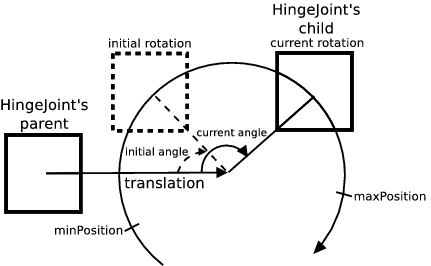
\includegraphics[width=0.6\textwidth]{figures/rotational_motor.png}
      \caption{Aktuatoren im Fahrradmodell.}
      \label{fig:aktuatoren}
    \end{figure}
    

  \begin{itemize}
    \item \textbf{Positionsmodus:} \\  
    Der Motor strebt einen vorgegebenen Zielwinkel an (\texttt{setPosition(angle)}), 
    wobei er innerhalb der konfigurierten Kraft- und Geschwindigkeitsgrenzen das nötige Drehmoment erzeugt, 
    um diesen Winkel zu erreichen. Dieser Modus entspricht einem Servomechanismus.  
    Im Webots-Modell ist der Lenkungsaktor in den Positionsmodus geschaltet.  
    Dazu wird im Code einmalig 
    \texttt{wb\_motor\_set\_position(handlebars\_motor, 0.0)} 
    aufgerufen, um die Start-Sollposition (geradeaus) zu setzen.  
    Anschließend erhält der Lenkmotor in jeder Regeliteration einen neuen Sollwinkel.  
    Die Regelung der Position übernimmt Webots intern: 
    der Motor wirkt wie eine Feder-Dämpfer-Kopplung ans Gelenk, 
    die Differenz zwischen Ist- und Sollwinkel generiert ein entsprechendes Gegendrehmoment (virtueller P-Regler).  
    Parameter wie \texttt{maxTorque} und \texttt{maxVelocity} im Weltfile bestimmen, 
    wie schnell und kräftig das Soll nachgeführt wird.  
    Im Modell sind z.\,B. für den Lenkmotor \texttt{maxTorque = 25\,Nm} festgelegt – 
    ein Wert, der sicherstellt, dass genügend Kraft zum Aufrichten aus Schräglagen vorhanden ist, 
    ohne das System zu unrealistisch zu machen.

    \item \textbf{Geschwindigkeitsmodus:} \\  
    Hier wird dem Motor eine Ziel-Angulargeschwindigkeit vorgegeben (\texttt{setVelocity(omega)}), 
    während die Position auf unendlich gesetzt wird (\texttt{setPosition(INFINITY)}).  
    In Webots bedeutet dies, dass der Motor keinen festen Endwinkel hat, sondern kontinuierlich dreht.  
    Der Antriebsmotor des Hinterrads wird so betrieben: 
    im Initialisierungscode wird \texttt{wb\_motor\_set\_position(wheel\_motor, INFINITY)} 
    aufgerufen, was den Wechsel in den Geschwindigkeitsmodus bewirkt.  
    Fortan interpretiert Webots den Befehl \texttt{wb\_motor\_set\_velocity(wheel\_motor, v)} 
    als Soll-Drehzahl (in Rad/s) für das Rad.  
    Intern wirkt wieder ein virtueller Regler, der das nötige Drehmoment aufbringt, 
    um diese Geschwindigkeit zu erreichen/halten (bis zum max. Drehmoment).  
    Im Weltmodell ist für den Hinterradmotor ein recht hohes maximales Drehmoment von 120\,Nm erlaubt, 
    um Beschleunigungsvorgaben schnell umsetzen zu können.  
    Allerdings ist die erreichbare Drehzahl in der Praxis auch durch die Antriebsspannung bzw. Webots-Parameter 
    \texttt{maxVelocity} limitiert.  
    In S-Kurven-Simulationen wurde typischerweise eine Grundgeschwindigkeit von ca. $3$–$5\,\mathrm{m/s}$ gefahren, 
    was durch den entsprechenden \texttt{velocity}-Wert in Rad/s vorgegeben wird.
    \item \textbf{Kraft-/Drehmomentmodus:}  
    Alternativ kann man in Webots Motoren auch direkt ein Drehmoment vorgeben 
    (\texttt{setTorque(t)}), um z.\,B. eigene Regelalgorithmen für die Positions- und Geschwindigkeitssteuerung umzusetzen.  
    In unserem Modell wird dieser Modus nicht explizit genutzt, 
    da die beiden in Steuerungsmodellen gängigen Modi bereits ausreichen.  
    Dennoch ist es wichtig zu wissen, dass Webots stets mit Kräften/Momenten rechnet: 
    Die Position- und Velocity-Modelle setzen letztlich ein solches Drehmoment um, 
    das aus der jeweiligen Referenzgröße berechnet wird.
  \end{itemize}


  Die beiden Motoren sind im Weltfile als Geräte \texttt{handlebars motor} und 
  \texttt{motor::wheel} deklariert und jeweils dem passenden HingeJoint zugeordnet. 
  Webots erlaubt es, mehrere Motoren pro Gelenk zu definieren, 
  doch hier ist jeweils nur einer aktiv. 

  Die Namensgebung \texttt{motor::wheel} für den Hinterradantrieb ist ein Spezialfall: 
  Das Präfix \texttt{::} dient dazu, den Motor vom gleichnamigen (per DEF) vorderen Rad zu unterscheiden, 
  welches ebenfalls als \texttt{wheel} benannt ist – so können Kollisionen in der Namensauflösung vermieden werden. 
  Im Controller-Code greift man dann genau mit diesem Namen zu.

  \subsubsection*{Rolle im Regelkreis}

  Die Aktuatoren setzen die vom Regler berechneten Sollgrößen in physikalische Bewegung um 
  und schließen damit die \textbf{Wirkkette des Regelkreises}. 
  Konkret berechnet der Balance-Controller in jedem Zeitschritt zwei Stellwerte:

  \begin{itemize}
    \item den \textbf{Lenksollwinkel} $\delta_{\text{sol}}$ 
    (aus dem PID-Regler + Vision-Überlagerung), und
    \item die \textbf{Antriebs-Sollgeschwindigkeit} $v_{\text{sol}}$.
  \end{itemize}

  Diese Sollwerte werden direkt an die Motoren übergeben. 
  Der Lenkwinkel-Sollwert stammt aus der Kombination des inneren und äußeren Regelkreises: 
  Wie in Abschnitt \textit{Sensoren} erläutert, fusioniert der Controller den 
  \textbf{Balance-Anteil} (zur Selbstausrichtung) mit dem \textbf{Vision-Anteil} 
  (zur Kurvenfahrt) zu einer endgültigen Vorgabe \texttt{final\_steer}. 
  Dieses \texttt{final\_steer} entspricht einem Winkel in Radiant, 
  der begrenzt auf den physikalisch möglichen Bereich ($\pm 0.524$\,rad) 
  an den Lenkmotor geschickt wird. 

  Der Hinterrad-Sollwert \texttt{target\_speed} wird ebenfalls bestimmt – 
  im aktuellen Konzept abhängig vom Lenkeinschlag 
  (starker Lenkeinschlag $\rightarrow$ automatische Reduktion der Grundgeschwindigkeit). 
  Damit fungiert der Balance-Controller gleichzeitig als einfacher 
  \textbf{Geschwindigkeitsmanager}, 
  der z.\,B. in Kurven abbremst, um die Balance nicht zu gefährden. 
  Die Berechnung von \texttt{target\_speed} erfolgt durch einen separaten Algorithmus 
  (\texttt{speed\_pid\_compute}), 
  der den Vision-Lenkbefehl in eine prozentuale Reduktion der Grundgeschwindigkeit umsetzt. 
  Alternativ könnte hier ein echtes Geschwindigkeits-PID auf Basis der Encoder-Daten stehen – 
  dies ist eine mögliche Erweiterung. 

  Sobald die Stellgrößen vorliegen, werden sie an die Motor-API übergeben. 
  Damit findet die \textbf{Regler-Ausgabe} statt: 
  Die Software schreibt die Sollwerte in die Motoren, 
  und die Physiksimulation reagiert, indem sie die entsprechenden Kräfte auf das Modell einleitet. 

  Der \textbf{Lenkmotor} dreht die Vorderradgabel proportional zum Regelfehler – 
  wenn das Fahrrad z.\,B. nach rechts kippt (positiver Rollwinkel), 
  verlangt der PID einen Lenkeinschlag nach rechts, 
  um einen stabilisierenden Lenkimpuls zu erzeugen 
  (das Rad wird unter den Schwerpunkt gesteuert, ähnlich wie man einen fallenden Besen durch Vorziehen stabilisiert). 
  Gleichzeitig berücksichtigt der Vision-Anteil, ob ggf. bewusst in eine Kurve gelenkt werden soll. 
  Die resultierende Motorbewegung ist somit eine Überlagerung aus Stabilisieren und Navigieren. 

  Der \textbf{Hinterradmotor} liefert währenddessen den Vortrieb: 
  Eine Grundgeschwindigkeit hält das Fahrrad in Bewegung 
  (was das Balancieren erleichtert, da dynamische Stabilisierungskräfte wirken), 
  und bei Bedarf wird verlangsamt. 
  Im Geradeausfall (Vision inaktiv) regelt der Balance-Controller sogar nur die Balance 
  und reduziert Geschwindigkeit auf ein Mindestmaß, falls keine Steuerkommandos kommen. 

  Insgesamt sorgen die Aktuatoren dafür, 
  dass die vom Regler vorgegebenen Stellgrößen (Lenkwinkel, Antriebskraft) 
  tatsächlich umgesetzt werden – 
  sie sind somit die finalen Ausführungselemente des Reglers. 
  Ohne ausreichende Aktuatorleistung könnte das beste Regelgesetz das Fahrrad nicht stabilisieren; 
  in der Simulation sind sie jedoch so gewählt, dass die Anforderungen erfüllt werden.

  \textbf{Implementierung und Code-Integration:} Die Ansteuerung der Motoren erfolgt im Balance-Controller (C-Code) nach Berechnung der Sollwerte. 
  Bereits während der Initialisierung werden die Motoren konfiguriert: 
  Listing~4 zeigt, wie der Lenkmotor und der Radmotor als Devices geholt und in die gewünschten Modi versetzt werden. 
  Für den Lenkantrieb wird die Position initial auf $0.0$ gestellt (\textit{Lenker gerade}). 
  Für den Hinterradantrieb wird \texttt{wb\_motor\_set\_position(wheel\_motor, INFINITY)} gesetzt, 
  was – wie oben beschrieben – den Geschwindigkeitsmodus aktiviert. 
  Beide Motoren würden standardmäßig mit \texttt{velocity = 0} starten; 
  der Hinterradmotor erhält später im laufenden Betrieb eine Startgeschwindigkeit (Basiswert). 

  Im Regelprozess selbst (Hauptschleife) werden dann die aktuellen Stellbefehle übergeben:

  \begin{lstlisting}[language=C,caption={Motorsteuerung im Regelkreis},label={lst:motorsteuerung}]
  wb_motor_set_position(handlebars_motor, -final_steer);
  wb_motor_set_velocity(wheel_motor, target_speed);
  \end{lstlisting}

  Dabei ist wichtig zu erwähnen, dass der Lenkwinkel mit negativem Vorzeichen gesetzt wird. 
  Dies rührt von der Achsdefinition her – je nach Koordinatensystem ist eine positive Rotation der Lenkachse evtl. 
  als Linkseinschlag definiert, während der Regler positive Werte als Rechtsdrehung interpretiert (oder umgekehrt). 
  Durch das Vorzeichen wird sichergestellt, dass z.\,B. ein positiver Reglerausgang 
  (Korrektur nach rechts) tatsächlich den Lenker nach rechts steuert. 
  Solche Vorzeichenkonventionen sind in der Modellierung zu beachten. 

  Der Wert \texttt{target\_speed} wird in Rad/Sekunde an das Hinterrad übergeben. 
  Um einen Eindruck zu geben: Eine Zielgeschwindigkeit von z.\,B. 4\,m/s entspricht 
  (bei $\sim$0.7\,m Raddurchmesser) ungefähr 11.4\,rad/s Winkelgeschwindigkeit. 

  Das Logging im Code zeigt typischerweise Werte um 10–15\,rad/s für die Grundgeschwindigkeit. 
  Nachdem die Sollwerte gesetzt sind, greift die Webots-Physik die neuen Sollwerte im nächsten Zeitschritt auf 
  und beschleunigt/verstellt die Motoren entsprechend. 
  Im Code werden nach dem Setzen der Motoren noch Statuspakete versendet und Logging betrieben, 
  was für die Aktuatorwirkung selbst aber keine Rolle mehr spielt.



  Insgesamt ist die Motoransteuerung in Webots sehr direkt – ein Funktionsaufruf genügt, 
  um das physikalische Stellglied zu beeinflussen. 
  Dies erlaubt es, die Regelalgorithmen unkompliziert mit der Simulationswelt zu koppeln. 
  Listing~4 fasst die wichtigsten Schritte zusammen. 
  Hier sind sowohl die Initialisierung (Modussetzen) als auch die Laufzeitschleifen der Motoren zu sehen, 
  mit deutschen Kommentaren erläutert. 
  Man erkennt, wie die Aktuator-Schnittstelle an die zuvor beschriebenen Regelungsgrößen gebunden ist: 
  \texttt{final\_steer} (in rad) geht an den Lenkmotor, 
  \texttt{target\_speed} (in rad/s) an den Radmotor. 
  Diese Werte stammen direkt aus der Regelung (siehe vorherigen Abschnitt) – 
  es findet keine weitere Transformation mehr statt, da die Größeneinheiten 
  konsistent mit dem Webots-Modell gewählt wurden.
  
  \begin{lstlisting}[style=wbt_c,caption={IMU-Initialisierung und -Abfrage im C-Controller (Balance-Regelung)},label={lst:imu3}]
    // Motoren-Devices abrufen
    handlebars_motor = wb_robot_get_device("motor::handlebars");
    wheel_motor     = wb_robot_get_device("motor::wheel");
    if (handlebars_motor == 0 || wheel_motor == 0) {
        exit(1);
    }
    // Initialisierung der Motoren
    // Lenkmotor: Positionsmodus, Startwinkel = 0 rad
    wb_motor_set_position(handlebars_motor, 0.0); 
    // Hinterradmotor: Geschwindigkeitsmodus aktivieren
    wb_motor_set_position(wheel_motor, INFINITY);    
    // (Velocity bleibt zunaechst 0, wird spaeter gesetzt)
    
    //...(im Reglerloop, nach PID/MPC-Berechnung von final_steer/target_speed)
    
    // Lenkantrieb: Soll-Lenkwinkel setzen 
    wb_motor_set_position(handlebars_motor, -final_steer); 
    // Radantrieb: Soll-Drehgeschwindigkeit setzen
    wb_motor_set_velocity(wheel_motor, target_speed);      
 
  \end{lstlisting}
  

  Durch diese Implementierung wird das Zusammenwirken aller Komponenten deutlich: 
  \textbf{Sensoren} (IMU, Kamera, Encoder) liefern den aktuellen Zustand, 
  der \textbf{Regler} (PID \& MPC) berechnet daraus Stellgrößen, 
  und die \textbf{Aktuatoren} (Motoren) führen diese Stellgrößen am physikalischen Modell aus. 
  Die Webots-Simulation ermöglicht es, all dies in einem deterministischen Umfeld zu testen – 
  etwaige Fehlanpassungen (wie zu schwache Motoren oder unzureichende Sensorfrequenzen) 
  würden sofort im Verhalten sichtbar und könnten iterativ justiert werden, 
  bevor der Algorithmus auf einen realen Prototyp übertragen wird.



  \subsection{Controller}


  Ein Webots\mbox{-}Controller ist ein separates Programm (Prozess), das einen Roboter in der Simulation steuert 
  und über eine definierte API mit der Simulationswelt kommuniziert. Für jeden Roboter kann ein Controller in 
  C/C++, Python, Java oder MATLAB laufen, wobei Webots den Datenaustausch (Sensorwerte, Aktuatorbefehle) bei 
  jedem Simulationsschritt synchronisiert. Typischerweise durchläuft ein Controller eine Endlosschleife, in 
  der er Sensoren liest, Berechnungen durchführt und Aktuatoren ansteuert, wobei am Ende jeder Iteration die 
  Funktion \texttt{wb\_robot\_step()} aufgerufen werden muss. Dieser Aufruf übergibt die gewünschte 
  Control\mbox{-}Step\mbox{-}Dauer (in Millisekunden) an den Simulator und bewirkt, dass Webots die 
  Simulation um genau diesen Zeitschritt fortsetzt und dabei alle bis dahin vom Controller gesetzten 
  Befehle anwendet. Danach erhält der Controller die aktualisierten Sensorwerte des neuen Simulationszustands 
  zurück. Abbildung~3.6 veranschaulicht diese Synchronisation \cite{cyberbotics_controller_programming}.
  
  \begin{wrapfigure}{r}{0.5\textwidth} % r=rechts, l=links
    \vspace{-0.8\baselineskip}          % optional: nach Bedarf anpassen
    \centering
    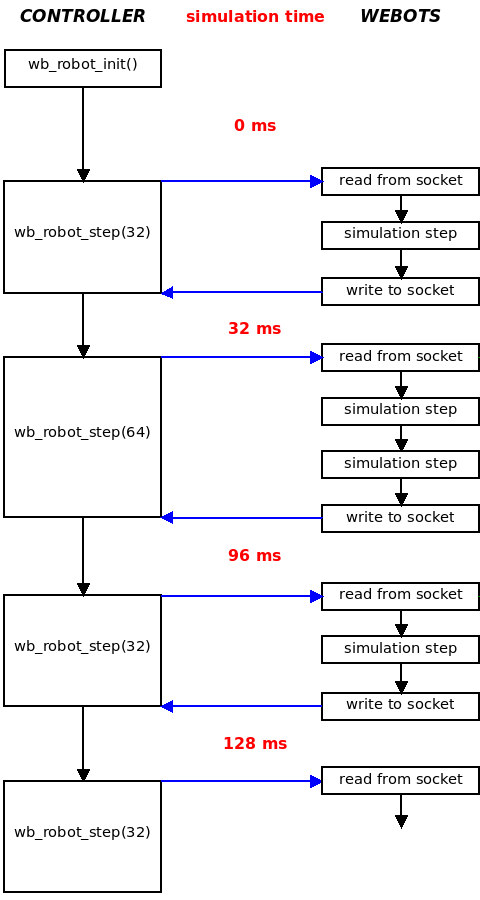
\includegraphics[width=\linewidth]{figures/controller_synchronization.png}
    \caption{Synchronisation zwischen Controller und Simulation.}
    \label{fig:controller_sync}
  \end{wrapfigure}


  Alle Anweisungen vor dem nächsten Zeitschritt (\texttt{wb\_robot\_step}\mbox{-}Aufruf) werden zunächst gesammelt; 
  mit dem Step\mbox{-}Aufruf rechnet der Simulator den nächsten Physikschritt und aktualisiert die Sensoren, bevor 
  der Controller weiterläuft. Auf diese Weise laufen Simulation und Controller \emph{synchron} in gleichmäßigen
   Zeitschritten. Standardmäßig wartet Webots in diesem synchronen Modus darauf, dass jeder Controller seinen \texttt{wb\_robot\_step} 
  ausführt, bevor der nächste Simulationsschritt erfolgt. Dies garantiert Konsistenz, erlaubt aber auch differierende Abtastraten: 
  Der Kontrollschritt muss ein ganzzahliges Vielfaches des Simulations\mbox{-}Basisschritts sein.

  Beispielsweise kann bei einer Weltzeit-schrittauflösung von 2\,ms ein Controller mit 2\,ms, 10\,ms oder 50\,ms 
  Schrittweite betrieben werden — Webots führt dann pro Controller-schritt entsprechend 1, 5 bzw.\ 25 Simulationsschritte 
  aus und wartet am Ende ggf.\ auf den Controller. Diese Entkopplung nutzt Webots, um auch langsamere Controller (z.\,B.\ in Python) 
  in eine schnelle Physiksimulation einzubetten, ohne die Synchronisation zu verlieren.

  Um auf Sensoren und Aktuatoren zuzugreifen, stellt Webots gerätespezifische API\mbox{-}Funktionen bereit. Im C\mbox{-}Controller 
  werden z.\,B.\ Geräte über \texttt{wb\_robot\_get\_device("name")} referenziert und Sensoren mit \texttt{wb\_sensor\_enable()} 
  aktiviert. Entsprechende Methoden existieren in Python (\texttt{robot.getDevice()}, \texttt{device.enable()}). Ein Sensor liefert 
  erst ab dem nächsten \texttt{wb\_robot\_step()} gültige Messwerte, da die Simulationszeit dann fortgeschritten ist. 

  Aktuatorbefehle (z.\,B.\ \texttt{wb\_motor\_set\_position()} oder \texttt{motor.setPosition()} in Python) werden zunächst lokal 
  gepuffert—die tatsächliche Ausführung in der Physik\mbox{-}Engine erfolgt erst am nächsten Step\mbox{-}Synchronisationspunkt. Daher 
  ist es sinnlos, in derselben Schleifeniteration zwei unterschiedliche Positionen für denselben Motor zu setzen: Nur der zuletzt vor 
  \texttt{wb\_robot\_step()} gesetzte Wert wird im kommenden Schritt ausgeführt. Ebenso bleiben zwei unmittelbar nacheinander gelesene 
  Sensorsamples identisch, solange kein Simulationsschritt dazwischen liegt. Dieses deterministische Schritt\mbox{-}für\mbox{-}Schritt\mbox{-}
  Ausführungsmodell erleichtert die Reproduzierbarkeit und verhindert \emph{race conditions} zwischen Physik und Reglercode.

  Für das selbstbalancierende Fahrrad wurden zwei Controller\mbox{-}Prozesse implementiert, die in Webots zeitgleich laufen und 
  über die oben beschriebene Mechanik gekoppelt sind: Einerseits der \emph{Balance\mbox{-}Controller} auf dem Fahrrad (in C, hoher Takt), 
  andererseits ein \emph{Vision\mbox{-}Controller} auf einem Supervisor\mbox{-}Knoten (in Python, langsamer Takt). Die Welt ist so 
  konfiguriert, dass das Fahrrad einen \texttt{Receiver} und einen \texttt{Emitter} trägt, während der Supervisor das komplementäre 
  Gegenstück besitzt; damit entsteht ein bidirektionaler Nachrichtenkanal innerhalb der Simulation:

  \begin{lstlisting}[style=wbt_c,caption={Nachrichtenkanal zwischen Controller und Simulation},label={lst:imu4}]
    Robot {
      Controller "balance_control_c"
      Receiver { name "command_rx"  channel 1  bufferSize 64 }
      Emitter  { name "status_tx"   channel 2  bufferSize 64 }
    }
    Supervisor {
      Controller "vision_control_py"
      Emitter  { name "command_tx"  channel 1  bufferSize 64 }
      Receiver { name "status_rx"   channel 2  bufferSize 64 }
    }
  \end{lstlisting}

  Über Channel 1 sendet der Vision-Controller Steuerkommandos an das Fahrrad, 
  und über Channel 2 übermittelt der Balance-Controller seinerseits Statusdaten zurück (z.\,B.\ aktueller Rollwinkel, Lenkwinkel, 
  Geschwindigkeit). Beide Controller laufen im \emph{synchronen Modus}, d.\,h.\ Webots hält die Physik so lange an, bis sowohl der 
  schnelle C-Controller (alle 2\,ms) als auch der langsamere Python-Controller ihren Schritt abgearbeitet haben \cite{cyberbotics_emitter}\cite{cyberbotics_receiver}. 
  Praktisch bedeutet dies: Der Balance\mbox{-}Regler berechnet bei jedem Simulationsschritt neue Motorbefehle, während der
  Vision\mbox{-}Algorithmus nur alle 25 Schritte (50\,ms) ein neues Lenkkommando liefert. Die folgenden Punkte fassen Aufgaben und Interaktion zusammen:

  \begin{itemize}
    \item \emph{Balance\mbox{-}Controller (C, 500\,Hz):} Liest hochfrequent IMU\mbox{-} (Rollwinkel) und Radsensoren aus, regelt 
    den Balancierwinkel mittels PID und steuert den Lenkmotor sowie den Antriebsmotor kontinuierlich an. Verarbeitet eingehende Sollkommandos 
    der Vision\mbox{-}Ebene (z.\,B.\ Lenkwinkel) und kombiniert sie mit dem internen Regleroutput. Sendet zyklisch seinen Status 
    (Stabilitätsmaß, aktuelle Geschwindigkeit etc.) über den Emitter aus. Bei Ausbleiben externer Kommandos hält er das Fahrzeug 
    selbständig im Gleichgewicht (Fallback auf reinen Balance\mbox{-}Modus).
    \item \emph{Vision\mbox{-}Controller (Python, \(\sim\)20\,Hz):} Läuft als Supervisor\mbox{-}Controller mit Zugriff auf globale 
    Informationen. Nutzt die am Fahrzeug montierte Kamera (Bildrate ca.\ 20\,Hz) zur Fahrbahnerkennung (z.\,B.\ YOLO\mbox{-}Segmentierung) 
    und berechnet auf dieser Basis einen Trajektorien\mbox{-} bzw.\ Lenksollwert mittels modellprädiktiver Regelung (MPC) oder wahlweise 
    eines PID. Dieses Sollkommando wird paketbasiert an den Balance\mbox{-}Controller gesendet (\texttt{Emitter} auf Kanal 1). Zudem 
    überwacht der Vision\mbox{-}Controller den empfangenen Fahrzeugzustand (\texttt{Receiver} auf Kanal 2), um die Regelgüte zu 
    beurteilen oder Logging durchzuführen. Gegebenenfalls passt er seine Fahrstrategie an (etwa Geschwindigkeitsanpassung bei großen Balance\mbox{-}Fehlern).
  \end{itemize}

  Durch diese Aufteilung konnte eine zweistufige Regelungsarchitektur realisiert werden: Der innere C\mbox{-}Regler stabilisiert 
  das Fahrrad auf kurzen Zeitskalen autonom, während der äußere Python\mbox{-}Regler in größeren Abständen Kurskorrekturen vorgibt. 
  Webots gewährleistet die Synchronisierung beider Teilprozesse, sodass Kommandos verlustfrei und deterministisch am 
  Step\mbox{-}Synchronisationspunkt ausgetauscht werden. Im Ergebnis reagiert das Gesamtsystem echtzeitnah auf Störungen 
  (Balance) und plant zugleich vorausschauend seine Fahrtrajektorie; die Kopplung konnte in der Simulation umfassend getestet 
  und für den späteren Hardware\mbox{-}Einsatz vorbereitet werden.




  \subsection{Angebundene GUI}


  Die Simulationsumgebung verfügt über ein tkinter\mbox{-}basiertes GUI\mbox{-}Kontrollzentrum, mit dem sich die Regelungsparameter 
  des selbstbalancierenden Fahrrads in Echtzeit anpassen und die Fahrdaten live überwachen lassen. Dieses GUI bietet eine benutzerfreundliche 
  Oberfläche, um während der laufenden Webots\mbox{-}Simulation Einstellungen zu ändern, ohne die Simulation unterbrechen zu müssen. 
  Es gliedert sich in mehrere Tabs, von denen insbesondere \enquote{Parameter} und \enquote{Monitoring} für die Laufzeitanpassung 
  und \mbox{-}beobachtung relevant sind. Im Folgenden wird erläutert, wie diese Tabs funktionieren und wie die Laufzeitanpassung 
  der Parameter sowie das Live\mbox{-}Monitoring umgesetzt sind.


  \textbf{Parameter-Tab \mbox{-} Laufzeitfähige Parameteranpassung:} Der Parameter\mbox{-}Tab ermöglicht die direkte Einstellung der Regelungsparameter während der Simulation. Über Slider und 
  Eingabefelder können z.\,B.\ PID\mbox{-}Reglergrößen (Kp, Ki, Kd) und andere Steuerungsgrößen komfortabel angepasst werden. Dabei werden die aktuellen Werte in Echtzeit im GUI angezeigt 
  und validiert, während der Nutzer sie ändert. Einzelne Parametergruppen (etwa Winkel\mbox{-}PID, Geschwindigkeitsregelung, mechanische Limits) 
  sind übersichtlich gruppiert, sodass man nicht auf die Details jedes Parameters eingehen muss, aber einen strukturierten Überblick behält.

  Wesentlich ist, dass Änderungen unmittelbar wirksam werden, ohne die Simulation neu zu starten. Technisch geschieht dies durch ein 
  SON\mbox{-}basiertes Konfigurationssystem im Hintergrund. Das GUI lädt zu Beginn die aktuellen Parameter aus einer Konfigurationsdatei 
  (z.\,B.\ \texttt{balance\_config.json}) und schreibt geänderte Werte bei Bedarf zurück. Wird ein Wert verändert, kann der Nutzer die 
  neue Konfiguration speichern und anwenden (Schaltflächen \enquote{Speichern} bzw.\ \enquote{Anwenden} im GUI). Die laufende 
  Regelungssoftware erkennt diese Aktualisierung dank eines Hot\mbox{-}Reload\mbox{-}Mechanismus: Der Balance\mbox{-}Controller 
  lädt die JSON\mbox{-}Config in kurzen Intervallen oder auf Befehl neu, sodass geänderte Parameter sofort in den Regler einfließen.


  \textbf{Monitoring-Tab – Live-Datenvisualisierung und CSV-Logging: }Im \emph{Monitoring}-Tab werden Fahr- und Regeldaten \emph{live} visualisiert, 
  um das Verhalten des Fahrrads während der Simulation nachvollziehen zu können. Abbildung 9 zeigt den Monitoring-Tab mit Echtzeitdiagrammen. 
  Der Tab bietet interaktive Plots, die zentrale Größen über der Zeit darstellen — etwa den Rollwinkel, den Lenkausgang des Reglers, die aktuelle 
  und Ziel-Geschwindigkeit sowie die PID-Regleranteile (P, I, D). Über Auswahlkästchen kann gezielt gesteuert werden, welche Kurven angezeigt werden, 
  um den Überblick zu behalten; beispielsweise lassen sich nur die Balance-Controller-Daten oder nur die PID-Terme ein- oder ausblenden. Zusätzlich 
  stehen Zoom-Regler zur Verfügung, um den dargestellten Zeitraum einzugrenzen und Details zu analysieren.

  Die Datengrundlage bilden CSV-Protokolldateien, die vom Balance-Controller während jeder Fahrt automatisch erzeugt werden. Jede Simulation 
  (bzw.\ Fahrt) wird lückenlos in einer Log-Datei festgehalten — mit Zeitstempel und den relevanten Mess- und Steuergrößen (u.\,a.\ Winkel, 
  Geschwindigkeiten, Reglerausgänge, Fehlerwerte). Der Monitoring-Tab listet diese Aufzeichnungen und ermöglicht sowohl das nachträgliche Laden 
  einer aufgezeichneten CSV-Datei als auch den Live-Stream der jeweils neuesten Datei. Im Live-Modus wählt das System automatisch die aktuell 
  von der Simulation beschriebene Log-Datei aus und aktualisiert die Plots fortlaufend; alternativ kann der Benutzer eine frühere Aufzeichnung 
  vollständig laden und visualisieren. In beiden Fällen normalisiert das GUI die eingelesenen CSV-Daten (z.\,B.\ Umrechnung von Radmaß in Grad 
  oder m/s in km/h) und zeichnet zweigeteilt: typischerweise erscheinen Winkel- und Lenkdaten im oberen Diagramm, die PID-Terme sowie Geschwindigkeiten 
  im unteren, jeweils mit gemeinsamer Zeitachse.
  \begin{figure}[H]
    \centering
    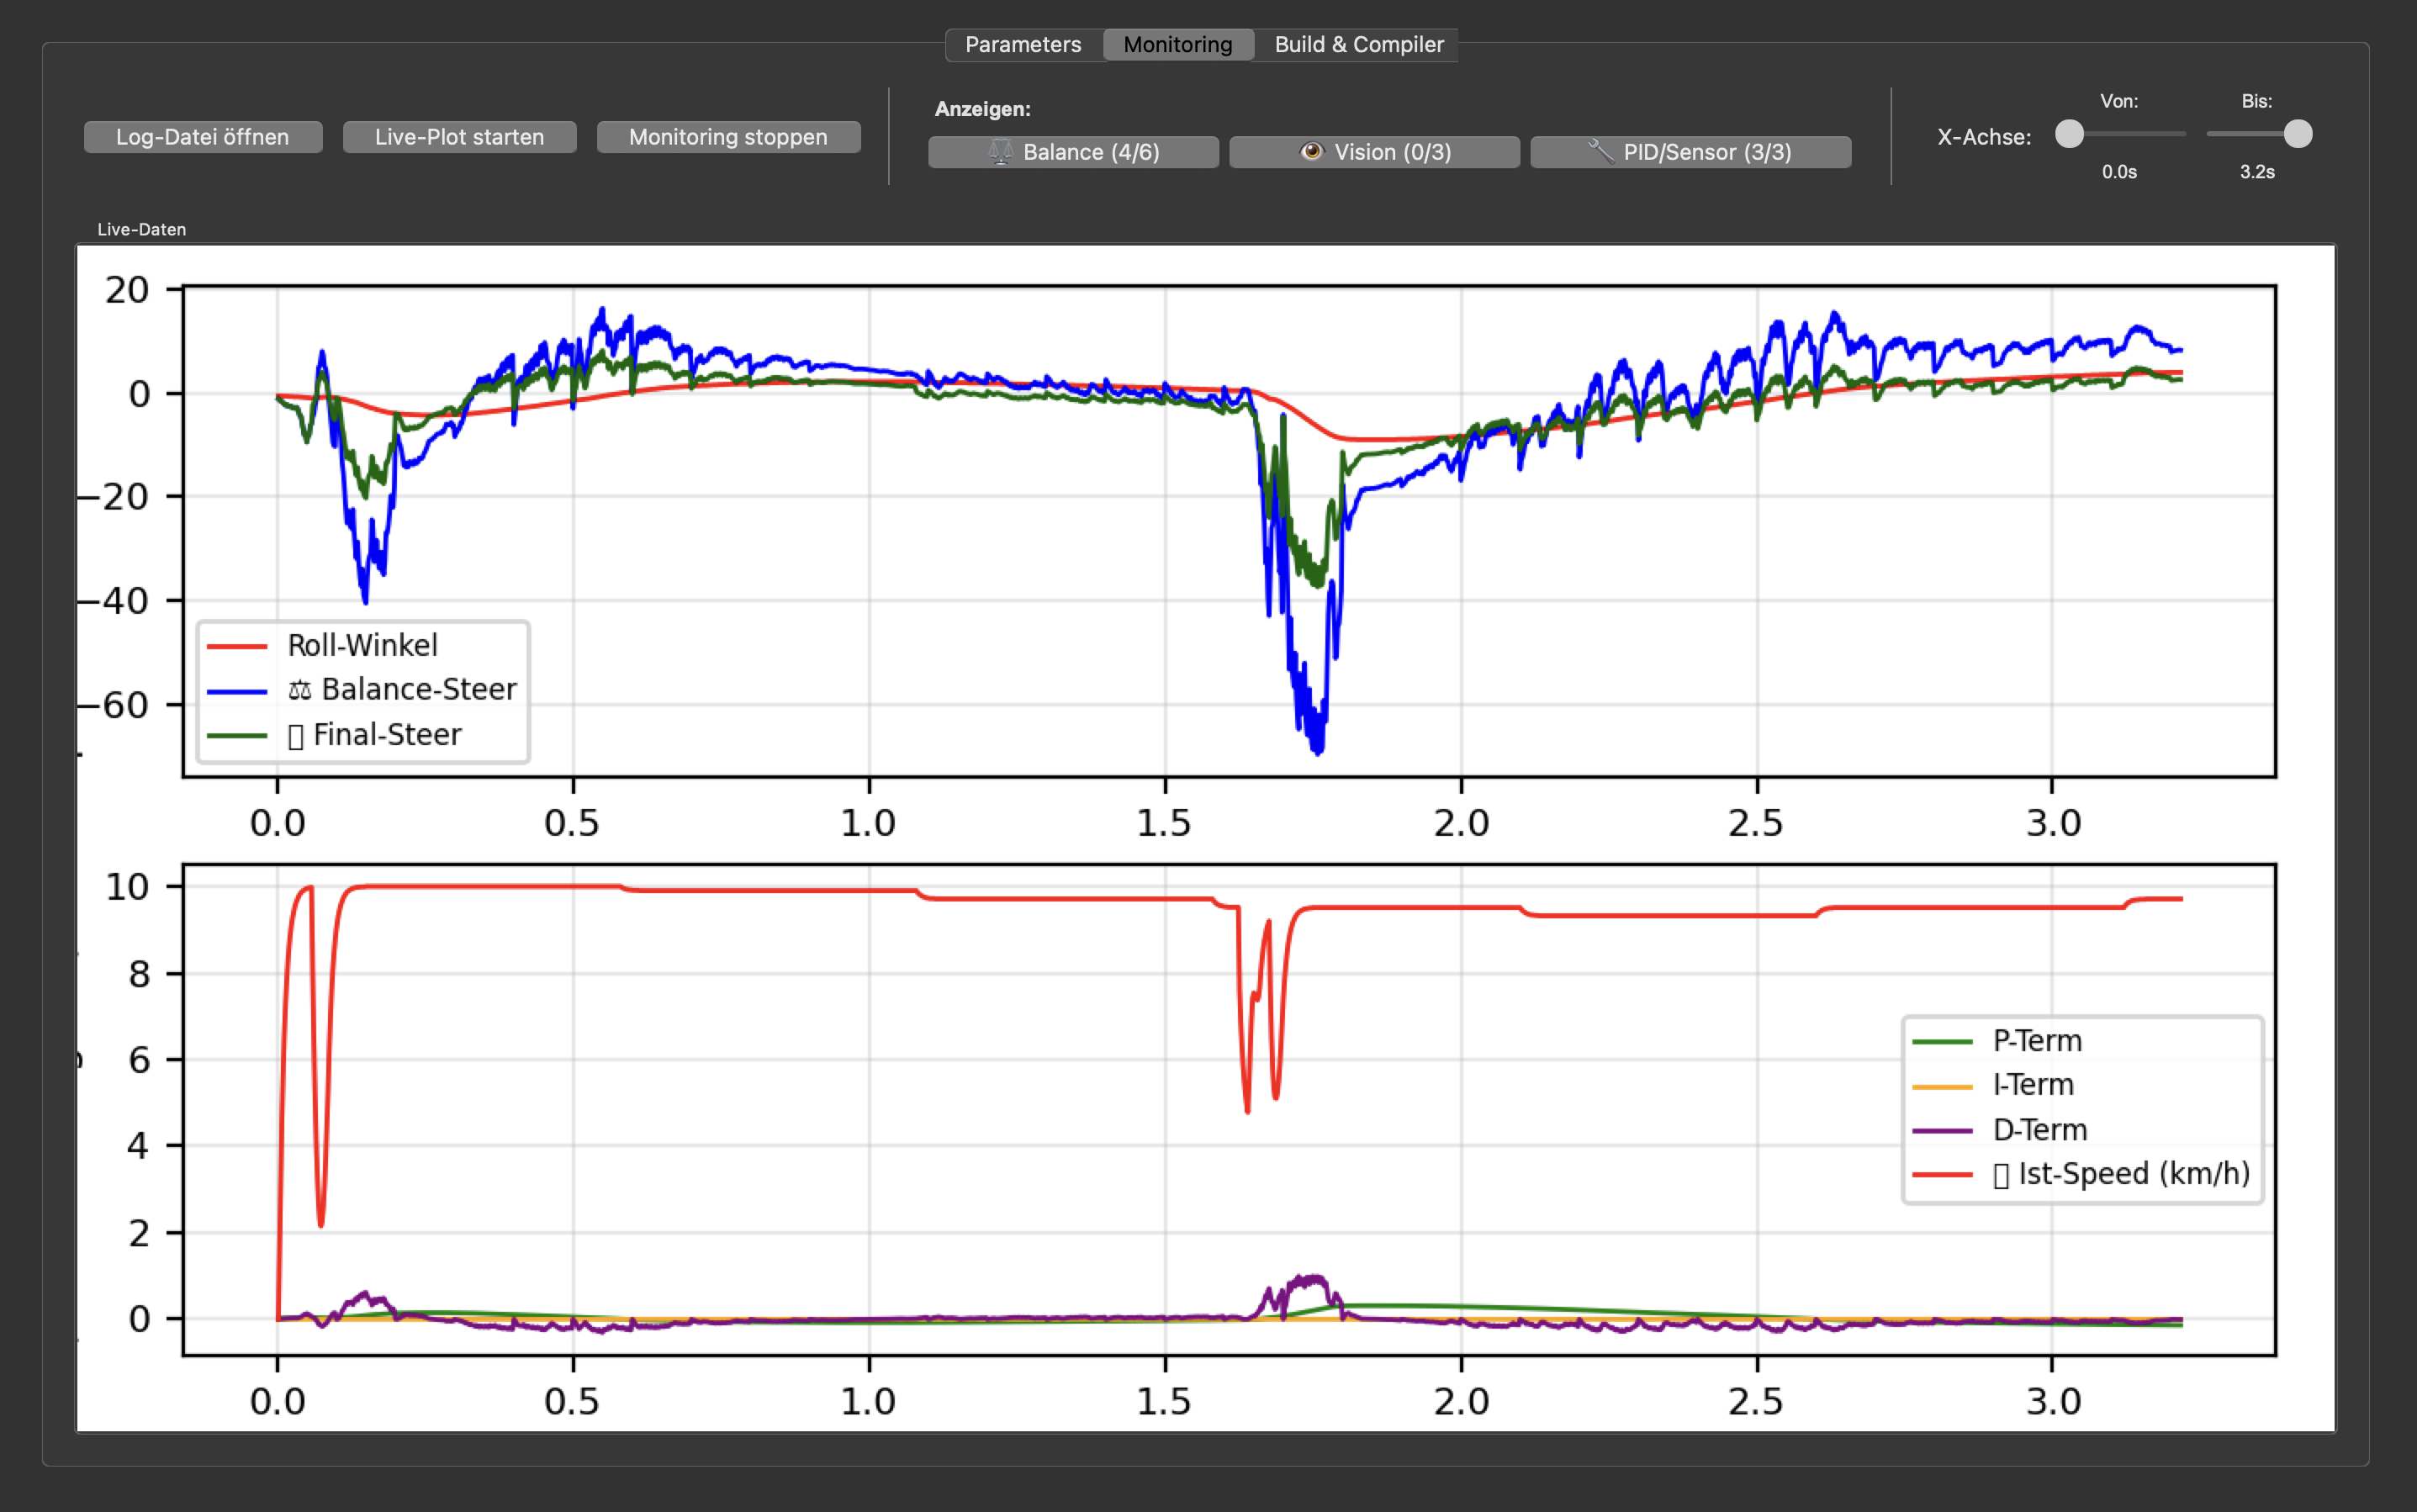
\includegraphics[width=1.0\textwidth]{figures/GUI_2.png}
    \caption{Monitoring-Tab mit Echtzeitdiagrammen.}
    \label{fig:GUI_2}
  \end{figure}

  Ergänzend zur grafischen Darstellung bietet der Monitoring-Tab Statusanzeigen, die u.\,a.\ den aktuell geladenen Logfile-Namen, den Zeitpunkt 
  der letzten Aktualisierung und den Laufzustand des Controllers ausweisen. So bleibt stets transparent, ob die Verbindung zur Simulation aktiv 
  ist und welche Datenquelle visualisiert wird. Zusammengenommen stellt der Monitoring-Tab ein leistungsfähiges Werkzeug dar, um die Auswirkungen 
  von Parameteränderungen sofort sichtbar zu machen und das Systemverhalten mittels aufgezeichneter Daten zu analysieren. Die Kombination aus
  laufzeitfähiger Parameteranpassung und Live-Monitoring ermöglicht ein effizientes Trial-and-Error-Tuning des selbstbalancierenden Fahrrads, 
  unterstützt durch intuitive GUI-Interaktion und automatisierte Datenaufzeichnung.

 






%--------------------------------------------------
% Kombinierte Regelung
%--------------------------------------------------
  \section{Kombinierte Regelung}
\subsection{Portierung des Balance-PID (Zander)}

Jonah Zanders Bachelorarbeit (2023) implementiert eine dreistufige Kaskadenregelung für ein selbstbalancierendes Fahrrad, die als Grundlage 
für die in dieser Arbeit entwickelte Simulationsregelung dient \cite{zander2023}. Die Hardware-Architektur umfasst einen BNO055-IMU-Sensor 
zur Neigungsmessung, einen BeagleBone-Black-Einplatinencomputer als Steuerungseinheit sowie separate Motorcontroller für Lenkung und Antrieb. 
Die Regelungsarchitektur gliedert sich in drei hierarchische Ebenen: eine primäre Balance-PID-Regelung (Angle-to-Steering), eine sekundäre 
Lenkpositionsregelung und eine vereinfachte Geschwindigkeitssteuerung.

\textbf{Primäre Balance-Regelung:} Das Kernstück von Zanders Implementierung bildet ein PID-Regler, der die Rollwinkelabweichung in einen 
Lenkwinkel-Sollwert umsetzt. Listing~\ref{lst:zander_pid_params} zeigt die von Zander gewählten PID-Parameter, die sich durch hohe 
proportionale (\(K_p = 10{,}0\)) und differentielle Verstärkungen (\(K_d = 2{,}2\)) bei deaktiviertem Integralanteil (\(K_i = 0{,}0\)) 
auszeichnen. Diese Parametrierung gewährleistet eine schnelle Reaktion auf Neigungsänderungen ohne die Gefahr des Aufschaukelns durch 
Drift-Integration.

\begin{lstlisting}[style=wbt_c,caption={PID-Parameter in Zanders Hardware-Implementierung},label={lst:zander_pid_params}]
//PID Angle to Steering
#define ANGLE_PID_KP                    10.0f
#define ANGLE_PID_KI                    0.0f
#define ANGLE_PID_KD                    2.2f 
#define ANGLE_PID_OUTPUT_MIN            -150.0f
#define ANGLE_PID_OUTPUT_MAX            150.0f
#define ANGLE_PID_INTEGRAL_MIN          -60.0f
#define ANGLE_PID_INTEGRAL_MAX          60.0f
\end{lstlisting}

Die PID-Berechnung in Zanders System implementiert eine zeitbasierte Integration und Differentiation mit Historien-Pufferung zur 
Rauschunterdrückung. Der Differentialterm wird über mehrere Zeitschritte gemittelt, um hochfrequente Störungen zu dämpfen, 
während der Integralterm durch Anti-Windup-Mechanismen begrenzt wird.

\textbf{Sekundäre Lenkpositionsregelung:} Die zweite Regelebene steuert den physischen Lenkmotor über einen MD49-Controller an, 
um den von der Balance-PID vorgegebenen Sollwinkel zu erreichen. Aufgrund der mechanischen Eigenschaften des Lenkantriebs 
(Reibung, Trägheit, Totzeit) sind hier deutlich höhere Verstärkungen erforderlich:

\begin{lstlisting}[style=wbt_c,caption={Lenkpositions-PID-Parameter in Zanders System},label={lst:zander_steering_pid}]
//PID Steering PID
#define MD49_PID_KP                     850.0f
#define MD49_PID_KI                     300.0f
#define MD49_PID_KD                     30.0f
#define MD49_PID_OUTPUT_MIN             -100000.0f
#define MD49_PID_OUTPUT_MAX             100000.0f
\end{lstlisting}

\textbf{Echtzeit-Threading-Architektur:} Zanders Implementierung nutzt eine multi-threaded Architektur mit unterschiedlichen 
Abtastraten: IMU-Datenerfassung mit 200\,Hz, Lenkpositionsregelung mit 1000\,Hz und Geschwindigkeitsregelung mit niedrigerer 
Frequenz. Watchdog-Mechanismen überwachen die Thread-Ausführung und gewährleisten die Systemstabilität bei Hardwareausfällen.

\textbf{Adaptierung für die Webots-Simulation:} Die Portierung von Zanders Balance-Regelung in die Webots-Simulationsumgebung 
erforderte eine systematische Vereinfachung der Hardware-spezifischen Komplexitäten bei Beibehaltung der regelungstechnischen 
Kernprinzipien. Die wesentlichen Unterschiede zwischen Hardware- und Simulationsimplementierung zeigt Tabelle~\ref{tab:zander_comparison}.

\begin{table}[H]
\centering
\caption{Vergleich zwischen Zanders Hardware-Implementierung und Webots-Simulation}
\label{tab:zander_comparison}
\begin{tabular}{|l|l|l|}
\hline
\textbf{Aspekt} & \textbf{Zander (Hardware)} & \textbf{Webots-Simulation} \\
\hline
Sensorik & BNO055 IMU, Rauschen & Idealer Rollwinkelsensor \\
Threading & Multi-threaded (200/1000 Hz) & Synchrone Hauptschleife \\
Lenkpositionsregelung & Separater MD49-PID & Direkter Motoranschluss \\
PID-Parameter & $K_p=10, K_i=0, K_d=2.2$ & Identische Werte \\
Ausgangsbegrenzung & $\pm 150$ (Hardware-Einheiten) & $\pm 0.3$ rad \\
\hline
\end{tabular}
\end{table}

Die Webots-Implementierung vereinfacht die Architektur erheblich durch Elimination der sekundären Lenkpositionsregelung. 
Listing~\ref{lst:webots_balance_pid} zeigt die zentrale Balance-Regelschleife, die direkt den Lenkwinkel setzt:

\begin{lstlisting}[style=wbt_c,caption={Vereinfachte Balance-PID-Implementierung in Webots},label={lst:webots_balance_pid}]
// 1. Roll-Winkel messen (idealisiert, ohne Rauschen)
float roll_angle = get_roll_rad_raw();

// 2. PID-Regelung: Roll-Winkel -> Lenkwinkel  
if (control_enabled) {
    steering_output = -pid_compute(&angle_pid, 0.0, roll_angle, current_time);
}

// 3. Lenkwinkel begrenzen
if (steering_output > config.mechanical_limits.max_handlebar_angle) 
    steering_output = config.mechanical_limits.max_handlebar_angle;
else if (steering_output < -config.mechanical_limits.max_handlebar_angle)
    steering_output = -config.mechanical_limits.max_handlebar_angle;

// 4. Direkter Motoranschluss (keine sekundaere Regelung)
wb_motor_set_position(handlebars_motor, -final_steer);
\end{lstlisting}

Der PID-Algorithmus selbst wurde von Zanders Implementierung adaptiert, jedoch mit verbesserter numerischer Stabilität. 
Während Zanders Code eine komplexe Historien-Verwaltung mit zirkulären Puffern verwendet, nutzt die Webots-Version eine 
vereinfachte Zeitberechnung basierend auf dem deterministischen Simulationszeitschritt:

\begin{lstlisting}[style=wbt_c,caption={Vereinfachte PID-Berechnung in der Webots-Implementierung},label={lst:webots_pid_compute}]
// I-Term (Integral) - vereinfachte Zeitberechnung
int prev_index = (pid->history_counter + HISTORY_LEN - 1) % HISTORY_LEN;
float dt = (pid->time_history[pid->history_counter] - 
           pid->time_history[prev_index]) / 1000000.0; // Mikrosekunden -> Sekunden

if (dt > 0.0 && dt < 1.0) {  // Plausibilitaetspruefung
    pid->integral_term += pid->Ki * error * dt; 
}

// D-Term mit gleitendem Durchschnitt (wie bei Zander)
float current_derivative = (error - pid->error_history[prev_index]) / dt;
pid->derivative_history[pid->history_counter] = current_derivative;

float derivative_sum = 0.0;
for (int i = 0; i < HISTORY_LEN; i++) {
    derivative_sum += pid->derivative_history[i];
}
pid->derivative_term = pid->Kd * (derivative_sum / HISTORY_LEN);
\end{lstlisting}

Die erfolgreiche Übertragung von Zanders Regelungskonzept in die Simulation bestätigt 
die Robustheit des gewählten PID-Ansatzes. Die identischen Parameter (\(K_p = 10\), \(K_i = 0\), \(K_d = 2{,}2\)) erzielen 
auch in der idealisierten Webots-Umgebung stabile Balance-Regelung. Der Verzicht auf den Integralanteil erweist sich als 
vorteilhaft, da er Drift-bedingte Instabilitäten vermeidet, was ein Aspekt, der sowohl in der Hardware- als auch in der 
Simulationsumgebung relevant ist.

Die Portierung demonstriert, wie Hardware-spezifische Komplexitäten (Multi-Threading, Sensor-Rauschen, Aktor-Totzeiten) in 
einer Simulationsumgebung abstrahiert werden können, ohne die regelungstechnischen Kernprinzipien zu beeinträchtigen. 
Diese Vereinfachung schafft die Grundlage für die Integration zusätzlicher Regelungsebenen, insbesondere der vision-basierten 
Pfadführung, die in den folgenden Abschnitten behandelt wird.


  
\subsection{Portierung des Fahrtrichtungs-MPC (Giray)} \label{chap:MPC_KAPITEL}
Yasin Giray entwickelte in seiner Masterarbeit einen vision-basierten 
Fahrtrichtungsregler auf Basis von Model Predictive Control (MPC), 
um das selbstbalancierende Fahrrad autonom der Fahrspur folgen zu lassen \cite{vision_mpc_readme}. Dieser Regler modelliert die Fahrzeugdynamik mittels Einspurmodell 
und nutzt zwei Steuergrößen, die aktuelle Geschwindigkeit \(v\) und Lenkwinkel \(\phi\) als Eingaben für die Prädiktion. Der MPC berechnet 
also auf Grundlage von \(v\) und Lenkeinschlag die Fahrzeugbewegung voraus. Für den prädiktiven Regler wird ein 
Zustandsvektor \(x=[x, y, v, \text{yaw}]\) (Position, Geschwindigkeit, Gierwinkel) und ein Eingangsvektor \(u=[\text{accel}, \text{steer}]\) 
definiert. Giray wählte einen Zeithorizont von etwa 2~s und formulierte ein Optimierungsproblem, das die Abweichung von einer Soll-Trajektorie 
minimiert sowie Steuerungsaufwand und -änderungen übernimmt. Die Kostenfunktion des MPC addiert quadrierte Abweichungen der Zustände und Eingriffe über den Horizont sowie eine 
Endzustands-Strafe, z.\,B. \(J=\sum (x^T Q x + u^T R u + \Delta u^T R_d \Delta u) + x_{\text{final}}^T Q_f x_{\text{final}}\) \cite{vision_mpc_readme}. 
Neben den Kosten werden physikalische Nebenbedingungen wie maximaler Lenkwinkel, Lenkwinkelrate und Geschwindigkeit im Optimierungsproblem 
berücksichtigt, um realistische Lösungen zu gewährleisten.

Wesentliche Voraussetzung für den Fahrtrichtungs-MPC ist eine geeignete Referenztrajektorie der Straße. Giray implementierte hierfür eine 
Computer-Vision-Pipeline auf Basis von YOLOv8-Segmentierung, welche im Kamerabild die befahrbare Straße und deren Verlauf erkennt. Aus den 
segmentierten Bilddaten wird eine Reihe von Stützpunkten der Fahrbahn extrahiert. Anschließend 
wird mittels Spline-Interpolation eine glatte Kurve durch diese Punkte gelegt, die als Referenzkurve für den MPC dient. Er simuliert auf Basis des Einspurmodells die Fahrzeugbewegung und berechnet die optimalen 
Steuerbefehle, damit das Fahrrad der Kurve bestmöglich folgt. In Girays Umsetzung wird der Regler zyklisch mit ca. 10 Hz ausgeführt (Tickrate 100 ms). 
Pro Zyklus initialisiert der Controller den aktuellen Fahrzeugzustand (Position, Geschwindigkeit, Orientierung) und berechnet aus der ersten Sollkurve 
einen Vorhersagepfad. Die Optimierung liefert dann eine Stellgrößen-Sequenz für Beschleunigung und Lenkwinkel. 
Tatsächlich wird nur der erste Lenkwinkel-Impuls umgesetzt (Receding Horizon Control), welcher als neuer Lenkbefehl an das Fahrzeug geht. 
Im nächsten Zyklus wird der MPC erneut mit aktualisiertem Zustand und ggf. angepasster Referenz gestartet. Giray konnte in Simulationen zeigen, 
dass der MPC-Regler das Fahrrad effektiv der vorgegebenen Spur folgen lässt. Die geplante Spline-Trajektorie und die vom MPC gefahrene 
Ist-Trajektorie in seiner Arbeit, stimmen dabei eng überein, was die Güte der prädiktiven Regelung belegt.


\textbf{Adaptierung für Webots-Simulation:} Die Portierung von Girays MPC-Konzept in die Webots-Umgebung erforderte eine systematische 
Anpassung an die spezifischen Anforderungen der Simulation und Integration mit dem vorhandenen Balance-Controller. Tabelle~\ref{tab:giray_comparison} 
zeigt die wesentlichen Unterschiede zwischen Girays theoretischem Ansatz und der Webots-Implementierung.

\begin{table}[H]
\centering
\caption{Vergleich zwischen Girays MPC-Konzept und Webots-Implementierung}
\label{tab:giray_comparison}
\begin{tabular}{|l|l|l|}
\hline
\textbf{Aspekt} & \textbf{Giray (Theorie)} & \textbf{Webots-Implementierung} \\
\hline
Prädiktionshorizont & N=20 (2\,s - 10\,Hz) & T=3 (0.3\,s - 20\,Hz) \\
Referenzgenerierung & Spline-Interpolation & Vereinfachte Korrekturtrajectorie \\
Zustandsvektor & $[x, y, v, \psi]^T$ & $[x, y, v, yaw]^T$ (identisch) \\
Eingangsvektor & $[a, \delta]^T$ & $[accel, steer]^T$ (identisch) \\
Regelfrequenz & 10\,Hz & 20\,Hz \\
Optimierer & CVXPY (theoretisch) & CVXPY (praktisch) \\
Integration & Standalone & Gekoppelt mit Balance-PID \\
\hline
\end{tabular}
\end{table}

Die Webots-Implementierung vereinfacht Girays Ansatz erheblich durch Reduzierung des Prädiktionshorizonts auf 3 Zeitschritte 
(\(\approx 0{,}3\,\mathrm{s}\)). Diese Entscheidung wurde aus Echtzeitgründen getroffen, da die Integration mit dem Balance-Controller 
eine höhere Regelfrequenz (20\,Hz) erfordert. Listing~\ref{lst:webots_mpc_init} zeigt die Initialisierung des MPC-Controllers 
mit den angepassten Parametern:

\begin{lstlisting}[style=python,caption={MPC-Controller Initialisierung in der Webots-Implementierung},label={lst:webots_mpc_init}]
def __init__(self):
    # MPC-Parameter (reduziert gegenueber Giray)
    self.NX = 4  # Zustandsvektor: [x, y, v, yaw]
    self.NU = 2  # Eingaenge: [accel, steer]
    self.T = 3   # Praediktionshorizont (reduziert fuer Echtzeitfaehigkeit)
    
    # Kostenmatrizen (aehnlich Girays Formulierung)
    self.R = np.diag([0.01, 0.01])      # Eingangskostenmatrix
    self.Rd = np.diag([0.01, 1.0])      # Eingangsdifferenzkostenmatrix
    self.Q = np.diag([1.0, 1.0, 0.5, 0.5])  # Zustandskostenmatrix
    self.Qf = self.Q                    # Terminale Kostenmatrix
    
    # Fahrzeugparameter (Bicycle-Modell)
    self.WB = 1.2  # Radstand [m] (Fahrrad)
    self.DT = 0.1  # Zeitschritt [s]
    
    # Physikalische Begrenzungen
    self.MAX_STEER = math.radians(30.0)  # Maximaler Lenkwinkel
    self.MAX_DSTEER = math.radians(20.0) # Maximale Lenkwinkelrate
    self.MAX_SPEED = 8.0                 # Maximale Geschwindigkeit
    self.MIN_SPEED = 0.5                 # Minimale Geschwindigkeit
\end{lstlisting}

Anstelle von Girays komplexer Spline-Interpolation aus Bildpunkten verwendet die Webots-Implementierung eine vereinfachte 
Referenzgenerierung basierend auf dem aktuellen Vision-Fehler. Die Referenztrajektorie wird aus dem lateralen Spurabweichungsfehler 
abgeleitet, indem ein Ziel-Gierwinkel berechnet und über den kurzen Horizont interpoliert wird.

\textbf{MPC-Optimierungsalgorithmus:} Die Webots-Implementierung folgt Girays theoretischer Formulierung bei der Lösung des 
Optimierungsproblems. Listing~\ref{lst:webots_mpc_solver} zeigt den Kern des MPC-Algorithmus:

\begin{lstlisting}[style=python,caption={MPC-Optimierungsalgorithmus in der Webots-Implementierung},label={lst:webots_mpc_solver}]
def linear_mpc_control(self, xref, xbar, x0):
    """Loest MPC-Optimierungsproblem"""
    try:
        x = cvxpy.Variable((self.NX, self.T + 1))
        u = cvxpy.Variable((self.NU, self.T))
        
        cost = 0.0
        constraints = []
        
        for t in range(self.T):
            cost += cvxpy.quad_form(u[:, t], self.R)
            
            if t != 0:
                cost += cvxpy.quad_form(xref[:, t] - x[:, t], self.Q)
            
            A, B, C = self.get_linear_model_matrix(
                xbar[2, t], xbar[3, t], 0.0)  # Linearisierung um Referenz
            constraints += [x[:, t + 1] == A @ x[:, t] + B @ u[:, t] + C]
            
            if t < (self.T - 1):
                cost += cvxpy.quad_form(u[:, t + 1] - u[:, t], self.Rd)
                constraints += [cvxpy.abs(u[1, t + 1] - u[1, t]) <= self.MAX_DSTEER * self.DT]
        
        cost += cvxpy.quad_form(xref[:, self.T] - x[:, self.T], self.Qf)
        
        # Randbedingungen
        constraints += [x[:, 0] == x0]
        constraints += [x[2, :] <= self.MAX_SPEED]
        constraints += [x[2, :] >= self.MIN_SPEED]
        constraints += [cvxpy.abs(u[0, :]) <= self.MAX_ACCEL]
        constraints += [cvxpy.abs(u[1, :]) <= self.MAX_STEER]
        
        # Problem loesen
        prob = cvxpy.Problem(cvxpy.Minimize(cost), constraints)
        prob.solve(verbose=False)
        
        if prob.status == cvxpy.OPTIMAL or prob.status == cvxpy.OPTIMAL_INACCURATE:
            u_opt = u.value
            if u_opt is not None:
                return u_opt[0, 0], u_opt[1, 0]  # Erste Kontrollaktion
        
        return self._simple_control_fallback(xref, x0)
        
    except Exception as e:
        return self._simple_control_fallback(xref, x0)
\end{lstlisting}

Die Implementierung folgt dem Standard-MPC-Schema mit quadratischen Kosten und linearen Constraints. Im Gegensatz zu Girays 
längerfristigem Horizont ermöglicht die Reduzierung auf 3 Zeitschritte eine Echtzeitausführung mit 20\,Hz.

\textbf{Integration mit Balance-Controller:} Ein wesentlicher Unterschied zu Girays Standalone-Ansatz liegt in der Integration mit 
dem bestehenden Balance-PID-Regler. Die Webots-Implementierung realisiert eine Kaskadenregelung, bei der der MPC-Controller die 
langfristige Spurführung übernimmt, während der Balance-PID die kurzfristige Stabilisierung gewährleistet. Die MPC-Ausgaben werden 
normalisiert und über IPC an den C-basierten Balance-Controller übertragen:

\begin{lstlisting}[style=python,caption={IPC-Übertragung der MPC-Kommandos an den Balance-Controller},label={lst:mpc_ipc}]
def send_vision_command(self, steer_cmd, speed_cmd):
    """Sendet erweiterte Vision-Command an Balance-Controller"""
    try:
        # Begrenzungen anwenden
        steer_cmd = max(-1.0, min(1.0, steer_cmd))
        speed_cmd = max(0.0, min(1.0, speed_cmd))
        
        # Erweiterte Struct-Format: 8 Felder
        # (steer_command, speed_command, valid, vision_error, 
        #  vision_p_term, vision_i_term, vision_d_term, mask_coverage)
        command_data = struct.pack('ffifffff', 
                                 steer_cmd, speed_cmd, 1,
                                 self.vision_error, self.mpc_controller.mpc_p_term, 
                                 self.mpc_controller.mpc_i_term, self.mpc_controller.mpc_d_term, 
                                 self.vision_mask_coverage)
        
        self.command_emitter.send(command_data)
        return True
    except Exception as e:
        return False
\end{lstlisting}

\textbf{Bewertung der Portierung:} Die Adaptation von Girays MPC-Konzept für die Webots-Simulation demonstriert sowohl die 
Übertragbarkeit theoretischer MPC-Ansätze als auch die Notwendigkeit praktischer Kompromisse.
Die vereinfachte Referenzgenerierung verzichtet auf Girays komplexe Spline-Interpolation, bietet jedoch ausreichende Genauigkeit 
für die Spurhaltung in der Simulation.

Die erfolgreiche Kopplung mit dem Balance-Controller zeigt, dass MPC-basierte Spurführung und PID-basierte Stabilisierung 
komplementäre Regelungsebenen darstellen können. Girays theoretischer Beitrag zur modellprädiktiven Fahrzeugführung findet 
somit praktische Anwendung in einem hybriden Regelungskonzept, das die Vorteile beider Ansätze kombiniert.

\newpage


\subsection{Strategien der Spurführung}

Die Vision-basierte Spurführung des selbstbalancierenden Fahrrads nutzt zwei unterschiedliche Erkennungsstrategien: 
eine YOLO-basierte Segmentierung als Hauptverfahren und eine robuste Fallback-Strategie für Ausfallsituationen. 
Beide Verfahren extrahieren aus dem Kamerabild einen lateralen Spurabweichungsfehler, der vom zuvor beschriebenen MPC 
in Lenkbefehle umgesetzt wird.

\subsubsection{YOLO-Segmentierung (YOLOv8)}

Die YOLO-Strategie nutzt ein vortrainiertes YOLOv8-Segmentierungsmodell zur robusten Erkennung der Fahrbahn. 
Das neuronale Netz identifiziert Straßenbereiche als Klasse \enquote{street\_main} und liefert sowohl Bounding Boxes 
als auch pixelgenaue Segmentierungsmasken, wie in Kapitel \ref{chap:yolo} beschrieben ist.
Das System sucht beim Start nach einer trainierten Gewichtsdatei (\texttt{best.pt}) 
und lädt das YOLOv8-Modell auf das verfügbare Rechengerät. Bei Nichtverfügbarkeit erfolgt automatischer Wechsel 
zur Fallback-Strategie:

\begin{lstlisting}[style=python,caption={YOLO-Modell Initialisierung},label={lst:yolo_init}]
  if YOLO_AVAILABLE:
    possible_paths = [
        "../balance_control_c/yolo_vision/runs/segment/train/weights/best.pt",
        "yolo_weights/best.pt",
        "best.pt"
    ]
    for path in possible_paths:
        if os.path.exists(path):
            try:
                device = "mps" if torch.backends.mps.is_available() else \
                         ("cuda" if torch.cuda.is_available() else "cpu")
                self.yolo_model = YOLO(path).to(device)
                print(f"[OK] YOLO-Modell geladen: {path} (Device: {device})")
                break
            except Exception as e:
                print(f"[WARN] Fehler beim Laden von {path}: {e}")
                continue
    if not self.yolo_model:
        print("[WARN] Kein YOLO-Modell gefunden - Fallback-Vision aktiviert")
        YOLO_AVAILABLE = False
\end{lstlisting}


Im Echtzeitbetrieb (20\,Hz) analysiert YOLO jedes Kamerabild und filtert Straßenobjekte 
(Klasse \enquote{street\_main}). Aus den Bounding Boxes aller erkannten Straßenbereiche wird der gemittelte Mittelpunkt berechnet. Die laterale 
Abweichung ergibt sich als normierte Differenz zwischen Straßenmittelpunkt und Bildmitte (\texttt{error} $\in [-0.5, +0.5]$):

\begin{figure}[H]
  \centering
  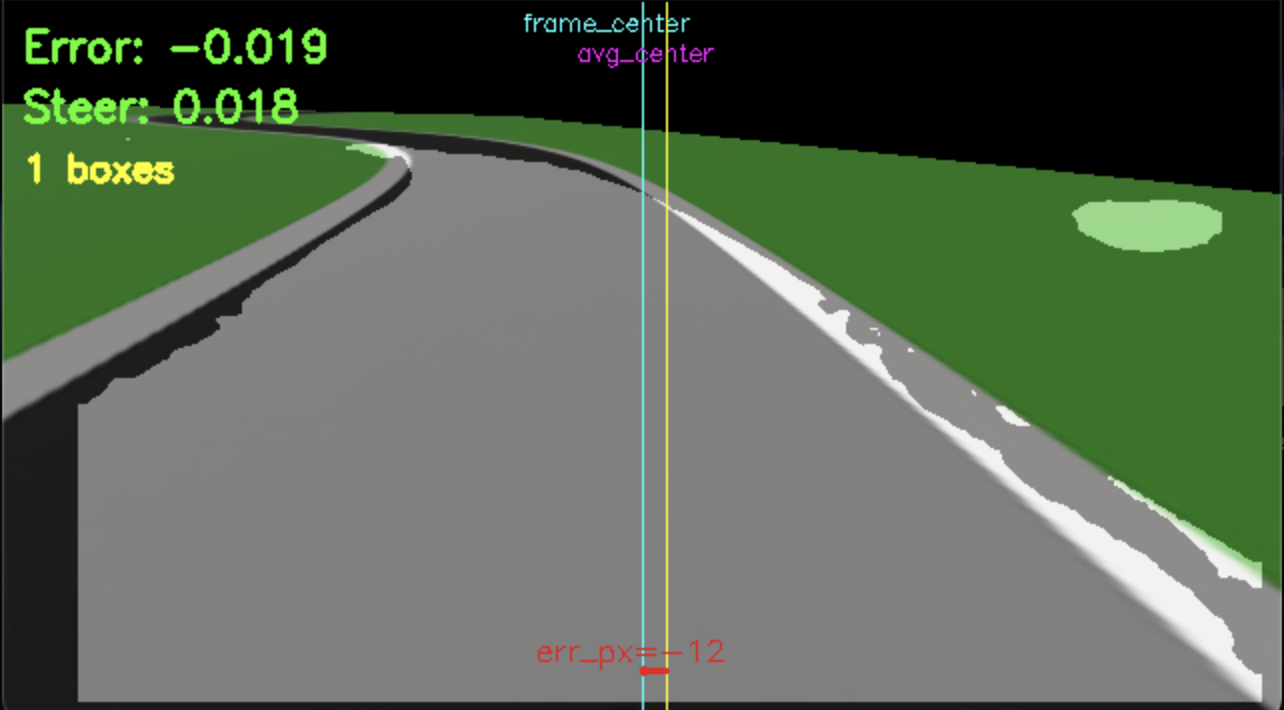
\includegraphics[width=0.8\textwidth]{figures/Yolo_Snapshot.png}
  \caption{YOLOv8-Segmentierung.}
  \label{fig:yolov8}
\end{figure}


\begin{lstlisting}[style=python,caption={YOLO-Fehlerberechnung},label={lst:yolo_error_calculation}]
  street_indices = [idx for idx, cls in enumerate(r.boxes.cls) if cls == 2]
  if street_indices:
      x_centers = []
      for idx in street_indices:
          xyxy = r.boxes.xyxy[idx]  # Koordinaten der Bounding Box
          x_center = float((xyxy[0] + xyxy[2]) / 2.0)
          x_centers.append(x_center)
      avg_x_center = sum(x_centers) / len(x_centers)
      frame_center = frame.shape[1] / 2
      error = (frame_center - avg_x_center) / frame.shape[1]  # Normiert
      self._store_valid_values(error, mask, self.vision_mask_coverage)
      return error, mask
\end{lstlisting}

Das System implementiert eine Ausfallüberbrückung durch Zwischenspeicherung 
der letzten gültigen Fehlerwerte. Bei Detektionsaussetzern wird der gespeicherte Fehler mit Decay-Faktor schrittweise 
abgeschwächt, bis er nach definierten Ausbleib-Zyklen auf Null fällt. Dies verhindert abrupte Lenkbewegungen bei 
temporären Erkennungsverlusten.




\textbf{Limitierungen:} Die YOLO-Strategie erfordert ein geeignetes vortrainiertes Modell und ausreichende 
Rechenleistung. Bei Abweichungen von den Trainingsdaten können Fehlerkennungen auftreten. Diese Fehlererkennungen 
werden in Kapitel \ref{chap:teststrecken} beschrieben. 



\subsubsection{Fallback-Strategie (ROI-basiert)}

Bei Nichtverfügbarkeit des YOLO-Modells aktiviert sich automatisch eine Fallback-Strategie, die auf klassischer 
Bildverarbeitung basiert. Diese nutzt Farb- und Konturfilter innerhalb einer definierten Region of Interest (ROI) 
zur Straßenerkennung, dabei mit geringerer Präzision, aber ohne Abhängigkeit von trainierten Modellen, bei 
denen zu fehlern bei der Straßenerkennung kommen kann.

\begin{figure}[H]
  \centering
  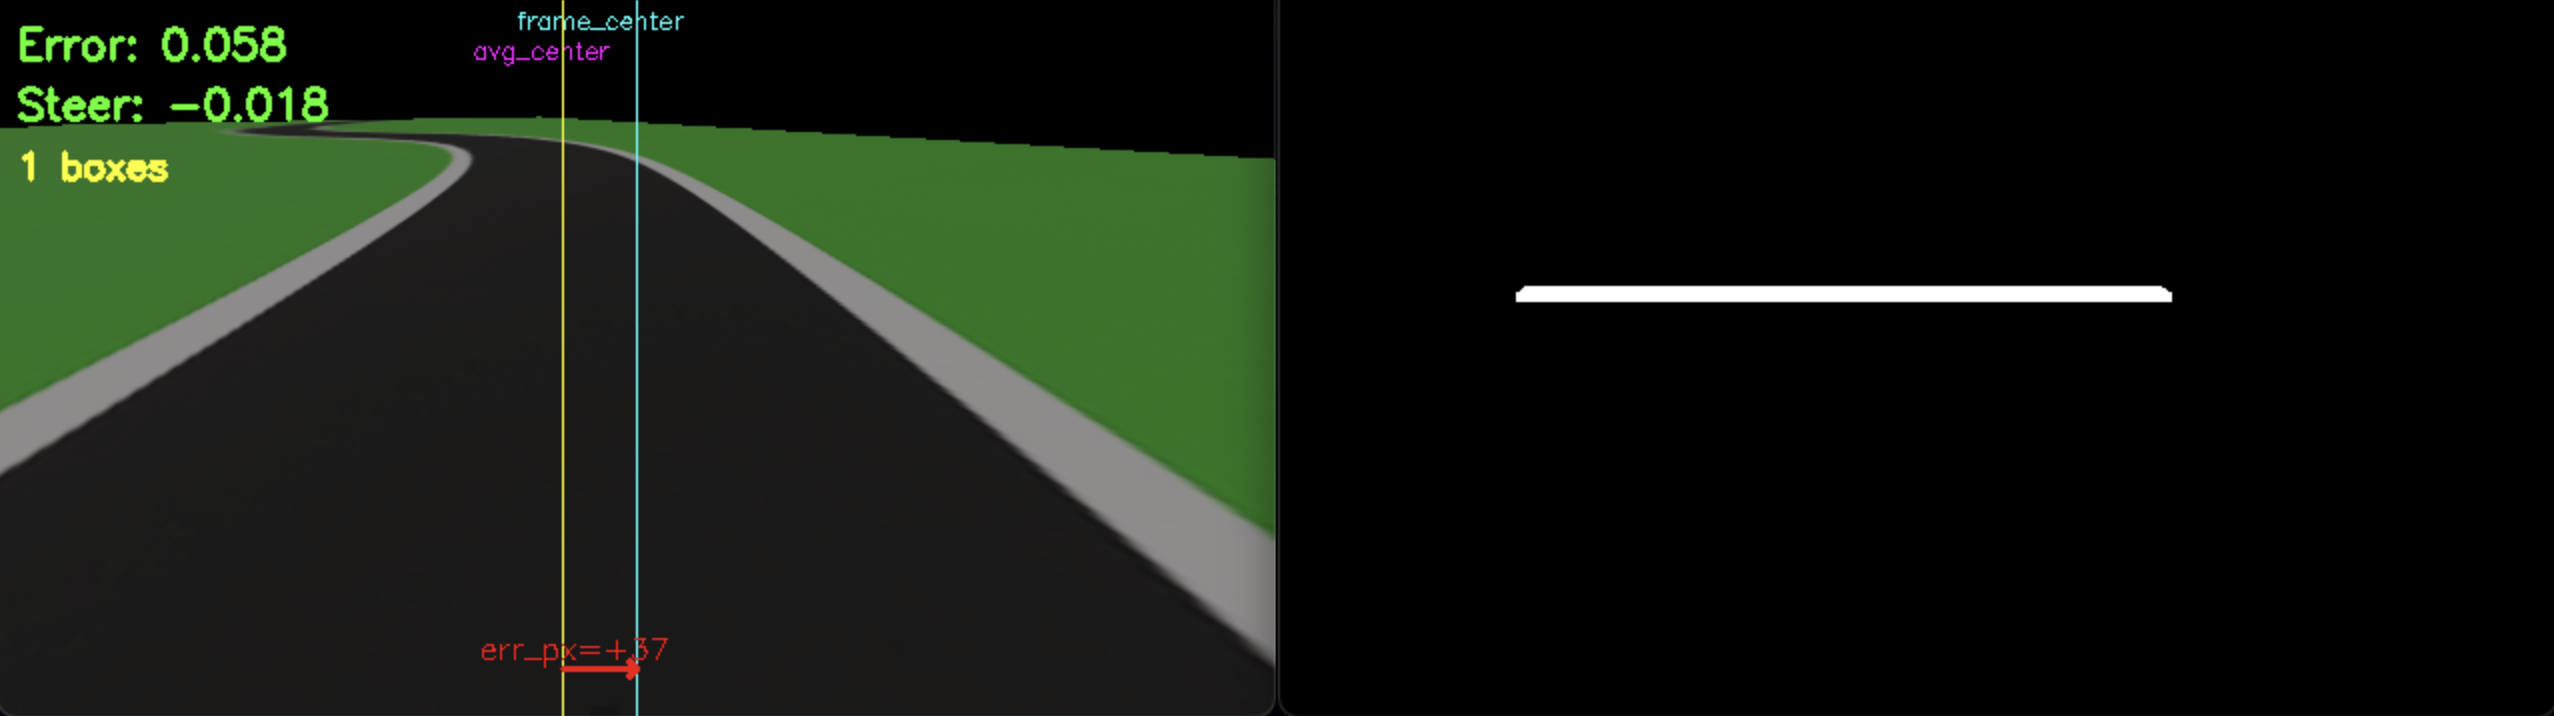
\includegraphics[width=1.0\textwidth]{figures/Fallback_snapshot.png}
  \caption{Fallback-Strategie.}
  \label{fig:fallback}
\end{figure}

Das System definiert eine trapezförmige ROI (ca.\ 40\% Bildhöhe, 2\% Breite) zur 
Fokussierung auf den erwarteten Fahrbahnbereich. Innerhalb dieser ROI erfolgt HSV-basierte Farbsegmentierung für 
dunkelgraue Straßenbereiche und weiße Markierungen, gefolgt von morphologischen Operationen zur Rauschreduktion. 
Die größte erkannte Kontur wird als Straßenbereich interpretiert:




\begin{lstlisting}[style=python,caption={Fallback-Fehlerberechnung},label={lst:fallback_error_calculation}]
  mask_road = cv2.inRange(hsv, road_lower, road_upper)      # Graue Strasse filtern
  mask_white = cv2.inRange(hsv, white_lower, white_upper)   # Weisse Markierungen filtern
  mask0 = cv2.bitwise_or(mask_road, mask_white)
  mask0 = cv2.morphologyEx(mask0, cv2.MORPH_CLOSE, kernel)
  mask0 = cv2.morphologyEx(mask0, cv2.MORPH_OPEN, kernel)
  contours, _ = cv2.findContours(mask0, cv2.RETR_LIST, cv2.CHAIN_APPROX_SIMPLE)
  if contours:
      largest_contour = max(contours, key=cv2.contourArea)
      x, y, w, h = cv2.boundingRect(largest_contour)
      center_x = int(x + w / 2)
      error = (x_set - center_x) / float(max(1, width))   # Fehler normiert an Bildbreite
      mask = np.zeros((height, width), dtype=np.uint8)
      cv2.drawContours(mask, [largest_contour], -1, 255, -1)
      ...  # (Berechnung der Maskenabdeckung)
      self._store_valid_values(error, mask, self.vision_mask_coverage)
      return error, mask

\end{lstlisting}

Der Algorithmus ermittelt die größte Kontur als Straßenbereich und berechnet deren Mittelpunkt. Die normierte 
Differenz zur Bildmitte ergibt den lateralen Fehler, analog zur YOLO-Methode. Bei Erkennungsverlusten greift 
die gleiche Decay-Logik wie in der YOLO-Strategie.

\textbf{Limitierungen:} Die Fallback-Strategie ist anfälliger für variierende Lichtverhältnisse und 
unkonventionelle Straßenbeläge, da sie auf feste Farbschwellenwerte angewiesen ist.
Trotz geringerer Präzision gewährleistet sie grundlegende Spurhaltung 
als Notfallmodus bei YOLO-Ausfall und ist besonders gut für vordefinierte Simulationswege geeignet.




%--------------------------------------------------
% Ergebnisse
%--------------------------------------------------
  \section{Ergebnisse}
\subsection{Fahrrad Datenblatt}

  Die folgenden Abschnitte beschreiben eine in Webots aufgebaute Simulation als digitalen Zwilling des realen Testfahrrads. Ziel ist, Masse-, Trägheits- und 
  Reibungsparameter sowie Sensor-/Aktorschnittstellen so realitätsnah zu spiegeln, dass das Fahrverhalten und die Reglerkopplung mit dem Prototyp übereinstimmen. 
  Auf Basis der ODE-Physik in Webots und der Controller-API (C/Python) wird die in der Hardware verwendete Architektur nachgebildet: eine schnelle innere 
  Balance-Schleife und eine langsamere, vision-gestützte MPC-Spurführung. Eine Supervisor-Instanz ermöglicht reproduzierbare Versuchsreihen, Resets und Logging, 
  sodass Parameterstudien und Kalibrierungen unter identischen Bedingungen erfolgen. Damit dient die Simulation als sichere Vorstufe für reale Fahrversuche und 
  als Referenz für die im Anschluss dokumentierten physikalischen Eigenschaften und Regelungsparameter.

  \begin{figure}[H]
    \centering
    
\includegraphics[width=1.0\textwidth]{figures/Datenblatt.png}  
    \caption{Datenblatt}
    \label{fig:datenblatt}
  \end{figure}
  
  \begin{itemize}
    \item \textbf{Masse und Schwerpunkt:} Der Rahmen des simulierten Fahrrads wiegt 3{,}5\,kg; zusammen mit den Rädern beträgt die Gesamtmasse ca. 5{,}1\,kg. 
    Der Schwerpunkt liegt etwa 5\,cm über dem Boden\gh, was ein stabiles Balanceverhalten begünstigt.
    
    \item \textbf{Trägheitssensor:} Im Webots--Modell ist der Trägheitssensor als Array in der Form
    \[
      [\,I_{xx}\; I_{xy}\; I_{xz}\; I_{xy}\; I_{yy}\; I_{yz}\; I_{xz}\; I_{yz}\; I_{zz}\,]
    \]
    angegeben. Für den Fahrradrahmen ergibt sich ein annähernd diagonal dominanter Trägheitstensor mit
    \(I_{xx}\approx I_{yy}=0{,}1\) und \(I_{zz}=0{,}05\,\mathrm{kg\,m^{2}}\)\gh. Der kleinere Wert um die Hochachse (Yaw-Trägheit) erleichtert schnelle 
    Lenkbewegungen; die Off-Diagonaleinträge sind Null, was bedeutet, dass die Hauptträgheitsachsen mit den Achsen des Modells ausgerichtet sind.
    
    \item \textbf{Räder:} Die beiden Räder haben einen Radius von 5{,}5\,cm und jeweils etwa 0{,}8\,kg Masse\gh. Durch die rotierende Masse entsteht ein 
    kleiner gyroskopischer Stabilisierungs-Effekt (Trägheitsmoment pro Rad ca. \(1\times10^{-3}\,\mathrm{kg\,m^{2}}\)), der zur Gesamtstabilität beiträgt, 
    aber aufgrund des geringen Werts nur begrenzten Einfluss hat\gh.
    
    \item \textbf{Reibungsparameter:} Die Radnaben besitzen eine viskose Lagerdämpfung (\texttt{dampingConstant} = 0{,}1) sowie Haftreibung (\texttt{staticFriction} = 0{,}1)\gh. 
    Diese Parameter simulieren Lagerveluste und verhindern z.\,B. ein freies Schwingen oder Durchrutschen der Räder im Stillstand. Zwischen Reifen und 
    Untergrund sorgt ein Coulomb-Reibungskoeffizient von etwa 0{,}8 für gute Traktion\gh; ein geringer Rückprallkoeffizient von 0{,}1 begrenzt die 
    Sprungelastizität des Reifenkontakts.
  \end{itemize}

  





\subsection{Teststrecken}
%------------------------------------------------------------------------------------------------
%------------------------------------------------------------------------------------------------
\subsubsection{Kurvenfahrt}
  \begin{wrapfigure}{r}{0.40\textwidth}
    \vspace{-0.8\baselineskip}
    \centering
    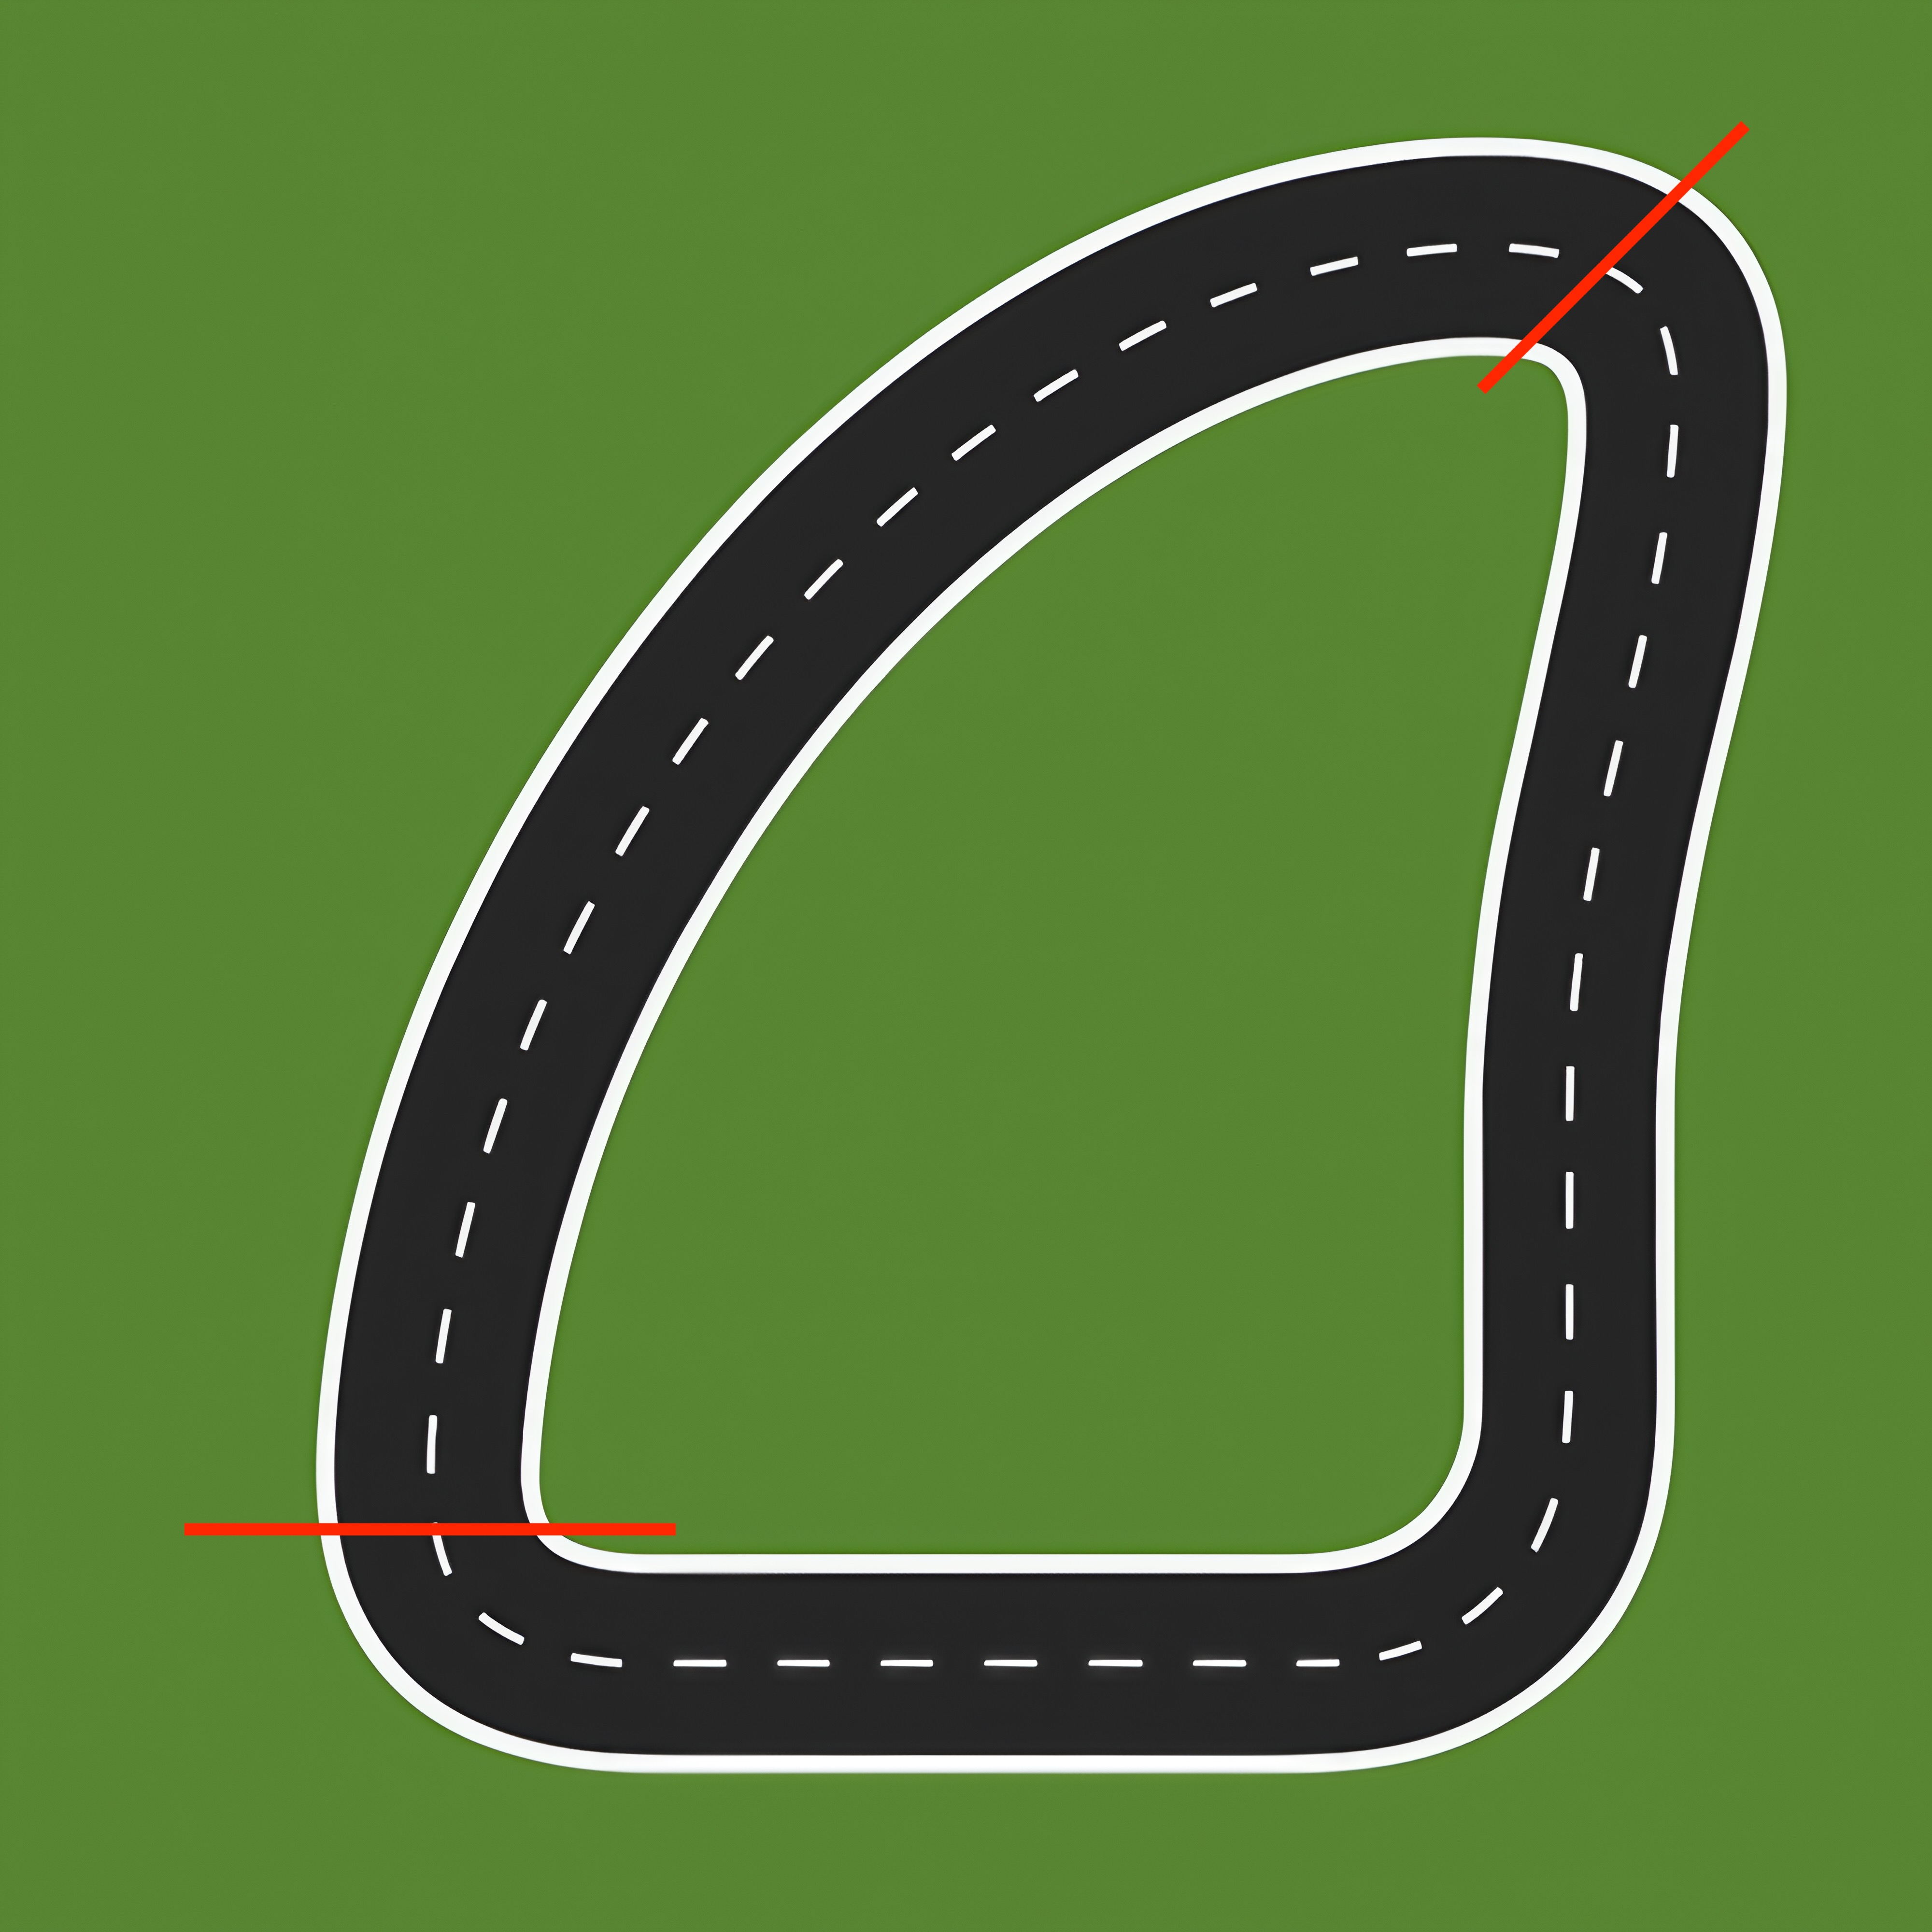
\includegraphics[width=\linewidth]{figures/Kurve.jpeg}
    \caption{Kurvenfahrt}
    \label{fig:kurvenfahrt}
  \end{wrapfigure}
  Die Fahrbahn ist als texturierte Ebene von 64m x 64m realisiert; die effektive Spurbreite beträgt an der 
  Referenzlinie etwa \SI{3.6}{\meter}. Die Strecke kombiniert eine lange Linkskurve (großer Radius) mit 
  einem engen Rechtsknick und eignet sich damit zur Bewertung von Spurtreue und Balance unter gekrümmter 
  Führung. Sofern nicht anders angegeben, sind für die Balance der \emph{PID}-Satz $K_p{=}2.0$, $K_i{=}0.2$, $K_d{=}0.5$, 
  der zulässige Lenkwinkelbereich $\delta\in[-0.3,\,0.3]\,\si{rad}$ 
  sowie $v_\text{base}{=}\SI{7}{km/h}$ (Grenzen \SI{5}{km/h} bis \SI{7}{km/h}) aktiv. 
  Mechanische Plausibilitätsgrenzen sind mit $\delta_\text{phys,max}{=}\SI{1.5}{rad}$ 
  und $\varphi_\text{roll,max}{=}45^\circ$ gesetzt. Für die visuelle Spurführung kann wahlweise 
  YOLO (Konfidenz 0{.}5) oder eine robuste ROI-Fallback-Erkennung verwendet werden (\texttt{roi\_top\_frac} = 0{.}5, 
  \texttt{roi\_height\_frac} = 0{.}06); Lenkbefehle werden durch \texttt{max\_delta} = 0{.}001 
  und \texttt{max\_steer\_cmd} = 0{.}06 geglättet und begrenzt. Ziel ist die Fahrt von der ersten 
  zur zweiten roten Markierung bei möglichst mittiger Spurhaltung und stabiler Balance.

  \paragraph{Einsatz eines vereinfachten Balance-P-Reglers}
  Für eine Baseline wurde der Balance-Regler auf einen reinen P-Anteil gesetzt ($K_p{=}2.0$, $K_i{=}0.0$, 
  $K_d{=}0.0$). \autoref{fig:kurvenfahrt-p} zeigt die gemessenen Größen der Fahrt, \autoref{fig:kurvenfahrt-p-error} 
  den zugehörigen ROI-Querfehler und \autoref{fig:kurvenfahrt-p-strecke} die Trajektorie auf der Strecke.
  \begin{figure}[H]
    \centering
    
\includegraphics[width=\textwidth]{figures/Kurve/Test P und PID/P/Daten.png}
    \caption{Kurvenfahrt mit reinem P-Regler (Zeitreihen)}
    \label{fig:kurvenfahrt-p}
  \end{figure}
  Bereits nach wenigen Sekunden setzt ein wachsendes Aufschaukeln ein: Der durch den Rollwinkel 
  induzierte Stellbefehl (\texttt{final\_steer}) treibt den Lenkeinschlag alternierend nach links/rechts, 
  bis die Phasenreserve erschöpft ist. Infolge der reinen Proportionalrückführung, der Aktuatorbegrenzungen 
  und der unvermeidlichen Latenzen entsteht ein unterdämpftes Verhalten; das Fahrrad kippt nach rund \SI{15}{\second} nach rechts.
  \begin{figure}[H]
    \centering
    
\includegraphics[width=\textwidth]{figures/Kurve/Test P und PID/P/Error.png}
    \caption{ROI-Querfehler während der P-Regler-Fahrt}
    \label{fig:kurvenfahrt-p-error}
  \end{figure}


  \begin{wrapfigure}{r}{0.40\textwidth}
    \vspace{-0.8\baselineskip}
    \centering
    
\includegraphics[width=\linewidth]{figures/Kurve/Test P und PID/P/Strecke.png}
    \caption{Gefahrene Trajektorie (P-Regler)}
    \label{fig:kurvenfahrt-p-strecke}
  \end{wrapfigure}


  Der ROI-Querfehler zeigt eine ausgeprägte Kopplung zum Rollwinkel: Das Pendeln der Balance überträgt sich 
  phasenverschoben auf die seitliche Abweichung. Zur Stabilisierung ist daher ein kleiner Integralanteil 
  (Elimination stationärer Abweichung mit Anti-Windup) und insbesondere ein Derivativanteil (Phasenführung/Dämpfung) 
  erforderlich; in Kombination mit Rate(\texttt{max\_delta}) und Amplitudenbegrenzung (\texttt{max\_steer\_cmd}) 
  wird das Überschwingen reduziert und ein Kippen verhindert.

  \clearpage
  \paragraph{Einsatz des erweiterten Balance-PID-Reglers}
  Für diese Versuchsfahrt wurden die erweiterten PID-Parameter $K_p = 2.0$, $K_i = 0.2$ und $K_d = 0.5$ eingesetzt. 
  Die Spurführung erfolgte mittels YOLO-basierter Bildverarbeitung. Während die Parameterwahl eine Verbesserung der 
  Stabilität gegenüber reinen P-Reglern bewirkte, zeigte sich nach etwa 35 s dennoch ein Kippen des Fahrrads, 
  ausgelöst durch abrupte Richtungsänderungen in der vom Vision-Modell vorgegebenen Trajektorie.
  \begin{figure}[H]
    \centering
    
\includegraphics[width=\textwidth]{figures/Kurve/Test P und PID/YOLO PID/Daten.png}
    \caption{Kurvenfahrt mit PID-Regler und YOLO-Spurführung}
    \label{fig:kurvenfahrt-pid-yolo}
  \end{figure}
  
  Die Fehleranalyse bestätigt, dass die Fahrbahnerkennung zum Zeitpunkt der Versuche noch unzureichend trainiert war. 
  Ab Sekunde 31 steigt der Querfehler abrupt an und fällt kurz darauf wieder ab (Sekunde 34). Dieses unstete Verhalten 
  überträgt sich auf den Rollwinkel, dessen zunehmendes Pendeln schließlich eskaliert und zum Umkippen des Fahrrads nach rechts führt.
  
  \begin{figure}[H]
    \centering
    
\includegraphics[width=\textwidth]{figures/Kurve/Test P und PID/YOLO PID/Error.png}
    \caption{ROI-Querfehler während der PID-Regler-Fahrt (YOLO)}
    \label{fig:kurvenfahrt-pid-error-yolo}
  \end{figure}

  \begin{wrapfigure}{r}{0.40\textwidth}
    \vspace{-0.8\baselineskip}
    \centering
    
\includegraphics[width=\linewidth]{figures/Kurve/Test P und PID/YOLO PID/Strecke.png}
    \caption{Gefahrene Trajektorie (PID-Regler mit YOLO)}
    \label{fig:kurvenfahrt-pid-strecke-yolo}
  \end{wrapfigure}

  Trotz dieser Limitierungen lässt sich durch die Kombination von Integral- und Differentialanteil eine verbesserte Spurhaltung 
  mit reduzierten Querabweichungen beobachten. Insbesondere werden stationäre Fehler kompensiert und Überschwinger wirksam gedämpft, 
  sodass das Fahrrad über weite Teile der Strecke stabil bleibt – auch bei eingeschränkter Fahrbahnerkennung. Kurz vor dem Ziel 
  versagt die Kompensation jedoch, und das System verliert seine Stabilität. Dies verdeutlicht, dass die Reglererweiterung eine 
  deutliche Verbesserung bewirkt, die Robustheit aber maßgeblich von der Qualität der visuellen Erkennung abhängt.

  \clearpage

  Die Abbildungen 24a und 24b verdeutlichen Limitierungen der \emph{YOLO}-Segmentierung: Abschnitte der Fahrbahn werden 
  nur teilweise bzw.\ falsch klassifiziert; insbesondere die Trennung zwischen Fahrbahn und Nebenflächen (z.\,B.\ Rand-/Grünstreifen) 
  ist inkonsistent. Links (a) ist die Spur weitgehend korrekt maskiert, rechts (b) werden Randbereiche fälschlich als Straße erkannt. 
  Diese Fehlklassifikationen verschieben die geschätzte Spurmitte, erzeugen sprunghafte Querfehler und können instabile Lenkbefehle auslösen.


  \begin{figure}[H]
    \centering
    \begin{subfigure}[t]{0.48\textwidth}
      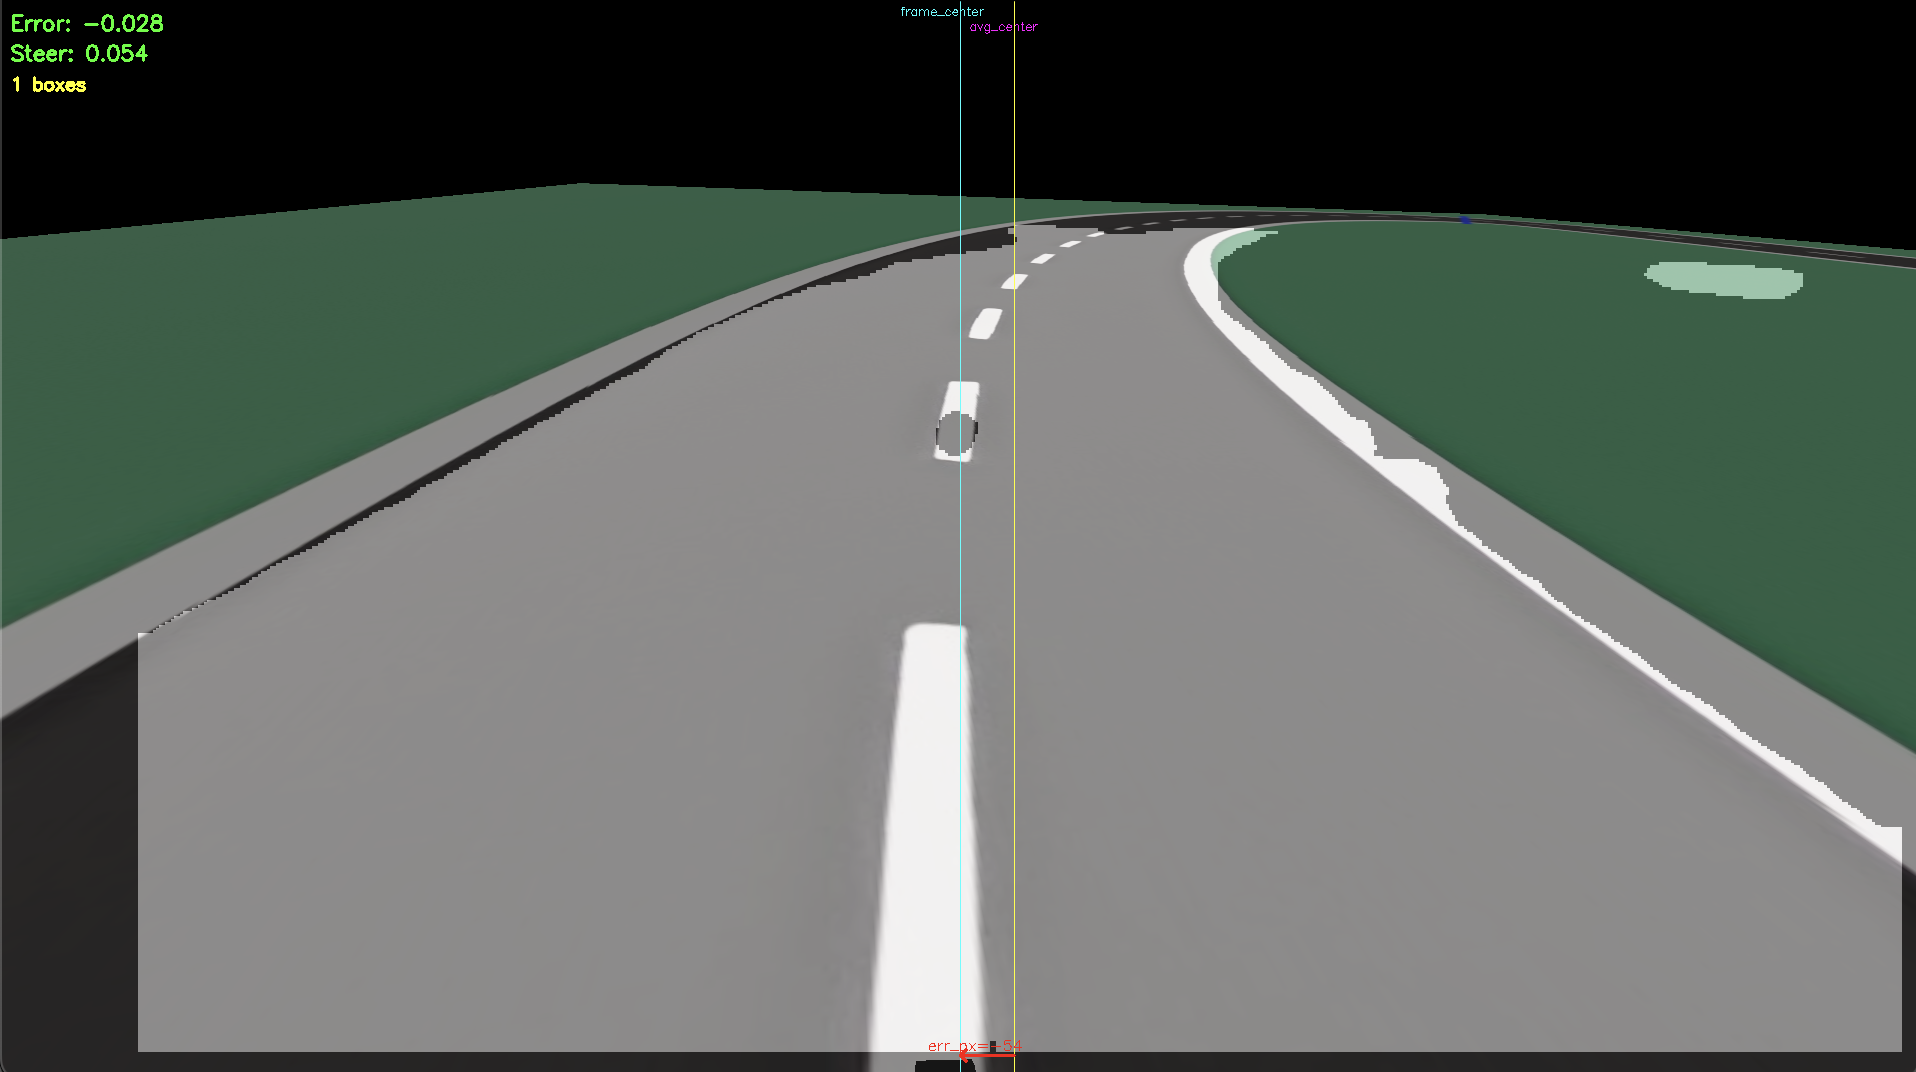
\includegraphics[width=\linewidth]{figures/Kurve/Test P und PID/YOLO PID/Strecke gut.png}
      \caption{Strecke gut}\label{fig:strecke-gut}
    \end{subfigure}\hfill
    \begin{subfigure}[t]{0.48\textwidth}
      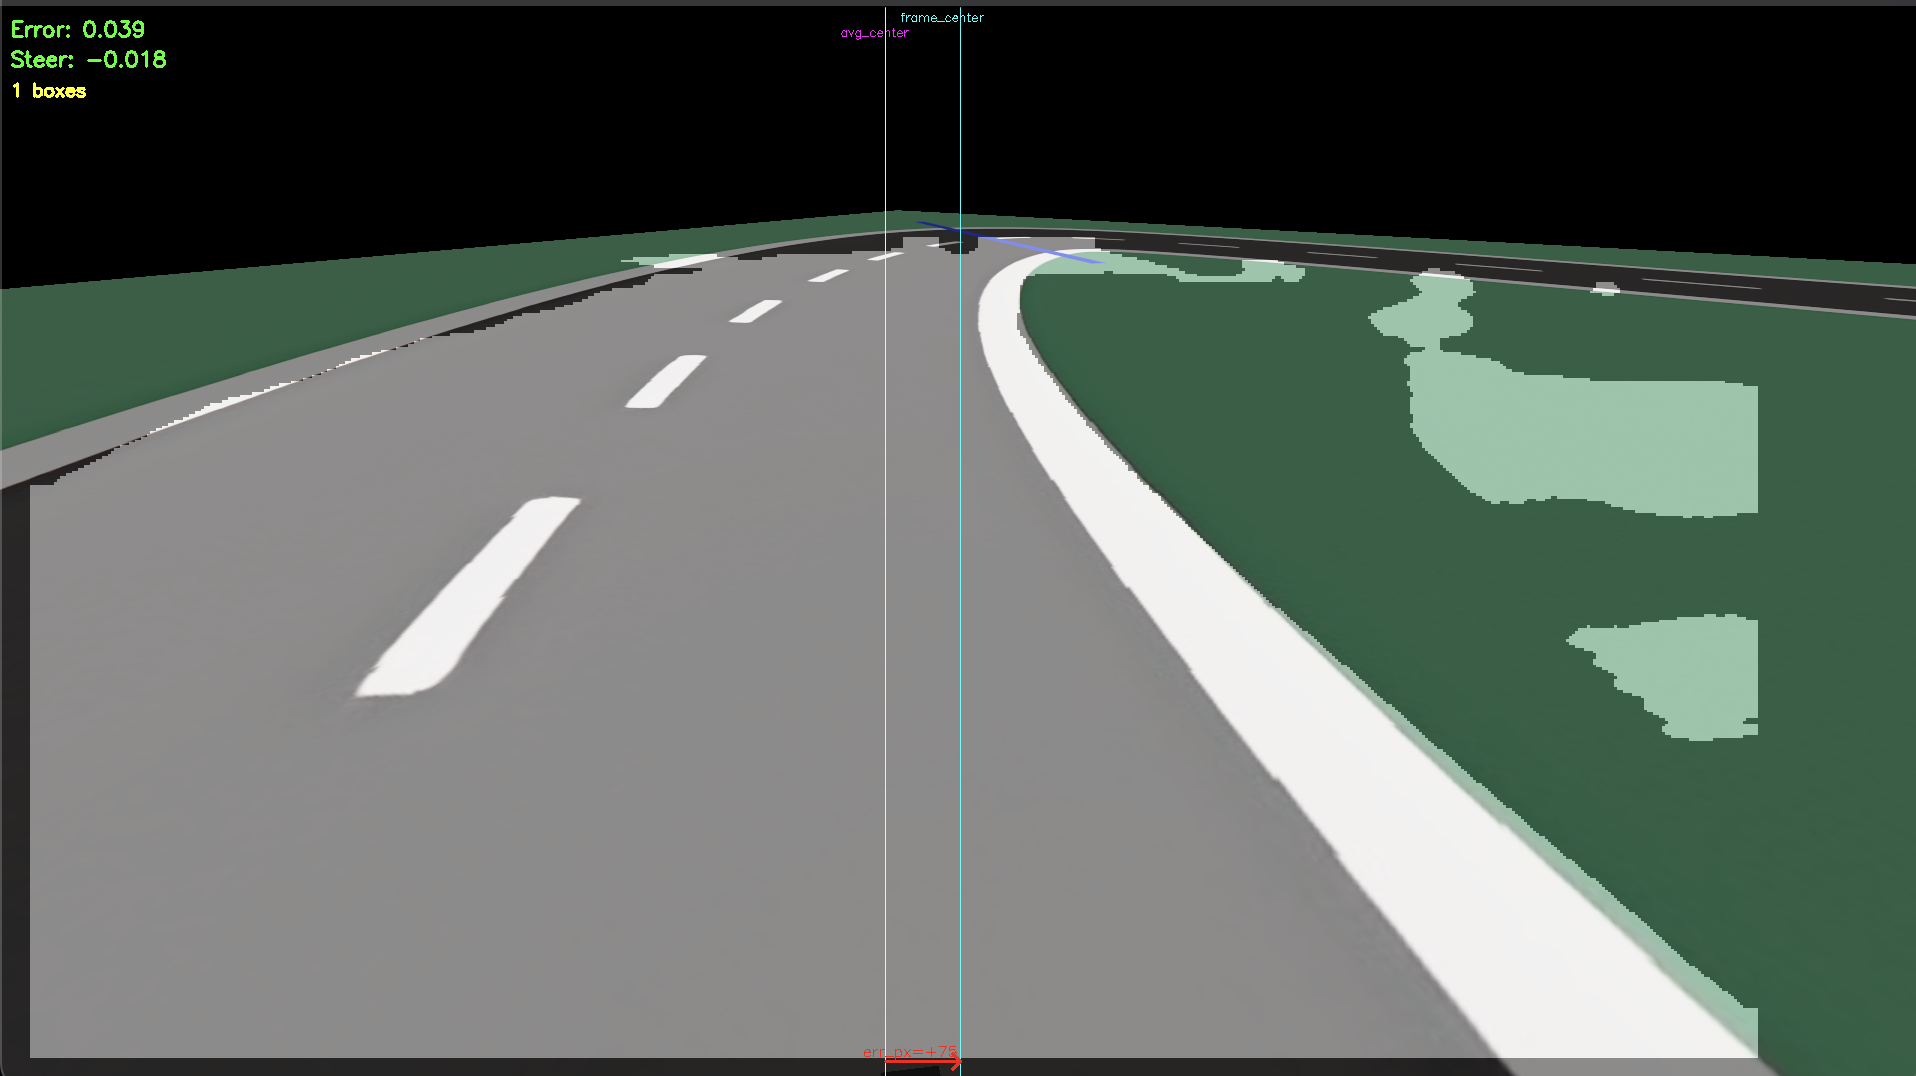
\includegraphics[width=\linewidth]{figures/Kurve/Test P und PID/YOLO PID/Stecke schlecht.png}
      \caption{Strecke schlecht}\label{fig:strecke-schlecht}
    \end{subfigure}
    \caption{Strecke gut und schlecht nebeneinander.}\label{fig:strecke-gut-schlecht}
  \end{figure}


  \paragraph{Einsatz der ROI\mbox{-}Fallback\mbox{-}Erkennung}
  In dieser Versuchsfahrt wurde die ROI\mbox{-}Fallback\mbox{-}Erkennung eingesetzt, um die in Abschnitt~4.3.1 beschriebenen Schwächen der \emph{YOLO}-Segmentierung zu umgehen. Die Pipeline nutzt klassische Bildverarbeitung innerhalb eines definierten Bildausschnitts (ROI): farbbasierte Segmentierung der Fahrbahn und Kantenfilter werden kombiniert, die Spurmittellinie wird aus der ROI-Maske abgeleitet und zeitlich geglättet. Sämtliche Reglerparameter (\emph{PID}) sowie die übrigen Versuchsbedingungen entsprechen exakt denen der YOLO-Konfiguration; die beobachteten Unterschiede sind daher allein auf die Wahrnehmung (Erkennung) zurückzuführen.
  
  \begin{figure}[H]
    \centering
    
\includegraphics[width=\textwidth]{figures/Kurve/Test P und PID/PID/Daten.png}
    \caption{Kurvenfahrt mit PID\mbox{-}Regler und ROI\mbox{-}Fallback\mbox{-}Erkennung}
    \label{fig:kurvenfahrt-pid-strecke-roi}
  \end{figure}
  
  Die Ergebnisse in \autoref{fig:kurvenfahrt-pid-strecke-roi} zeigen einen deutlichen Qualitätsgewinn gegenüber der YOLO\mbox{-}Erkennung: sprunghafte Querfehler treten praktisch nicht mehr auf, und das Fahrrad fährt über weite Strecken stabil. Kurzzeitige Anregungen (z.\,B.\ zwischen Sekunde~20 und~25) führen zwar zu einer temporären Erhöhung der Stellgrößen, werden jedoch vom PID\mbox{-}Regler sauber kompensiert. Der anfängliche Anstieg des \emph{Final\mbox{-}Steer} ist auf das Einfädeln in die Spur zurückzuführen; nach kurzer Transiente regelt sich das System auf einen kleinen stationären Fehler ein.
  
  \begin{figure}[H]
    \centering
    
\includegraphics[width=\textwidth]{figures/Kurve/Test P und PID/PID/Error.png}
    \caption{ROI\mbox{-}Querfehler während der PID\mbox{-}Regler\mbox{-}Fahrt (ROI)}
    \label{fig:kurvenfahrt-pid-error-roi}
  \end{figure}
  
  \begin{wrapfigure}{r}{0.40\textwidth}
    \vspace{-0.8\baselineskip}
    \centering
    
\includegraphics[width=\linewidth]{figures/Kurve/Test P und PID/PID/Strecke.png}
    \caption{Gefahrene Trajektorie (PID\mbox{-}Regler, ROI)}
    \label{fig:kurvenfahrt-pid-strecke}
  \end{wrapfigure}
  
  Im Fehlerverlauf (\autoref{fig:kurvenfahrt-pid-error-roi}) ist außerdem ersichtlich, dass ab etwa Sekunde~35 die (rote) Schwelle zur scharfen Kurve überschritten wird und der Querfehler ansteigt. Dieses Verhalten ist konsistent mit den in der Regelkette gesetzten Lenkwinkel- und Ratenbegrenzungen (\texttt{max\_steer\_cmd}, \texttt{max\_delta}): Bei hoher Streckenkrümmung gerät der Regler kurzzeitig in Sättigung, bevor der Fehler wieder abgebaut wird. Die zugehörige Trajektorie (\autoref{fig:kurvenfahrt-pid-strecke}) belegt dennoch eine insgesamt mittige und ruhige Spurhaltung; Abweichungen konzentrieren sich auf den Scheitel der Kurve und bleiben begrenzt.
  
  \smallskip
  \noindent\textit{Fazit.} Die ROI\mbox{-}Fallback\mbox{-}Erkennung erhöht die Robustheit der Spurführung, indem sie Ausreißer in der visuellen Messung reduziert und so die Kopplung zum Balance\mbox{-}Regelkreis entlastet. Ihre Wirksamkeit ist allerdings an Szenen mit gut trennbaren Fahrbahn-/Nebenflächen gebunden; für variable Beleuchtung, Texturen oder komplexe Hintergründe ist eine verbesserte (oder zusätzlich trainierte) lernbasierte Segmentierung weiterhin wünschenswert.
  

  \newpage

  






  %------------------------------------------------------------------------------------------------
  %------------------------------------------------------------------------------------------------

  \subsubsection{S-Kurve}


    \begin{figure}[H]
      \centering
      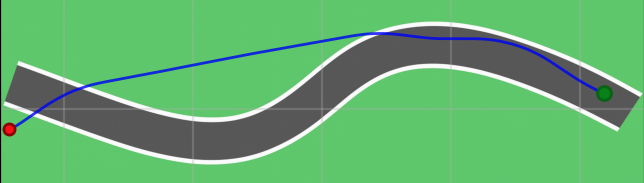
\includegraphics[width=1.0\textwidth]{figures/S-Kurve/Yolo_Strecke.png}  
      \caption{Fallback Strecke S-Kurve}
      \label{fig:fallback-strecke-s-kurve}
    \end{figure}

    \begin{figure}[H]
      \centering
      
\includegraphics[width=1.0\textwidth]{figures/S-Kurve/Fallback_Strecke.png}  
      \caption{Fallback Strecke S-Kurve}
      \label{fig:fallback-strecke-s-kurve}
    \end{figure}

   
    \begin{figure}[H]
      \centering
      
\includegraphics[width=1.0\textwidth]{figures/S-Kurve/Yolo_Daten.png}  
      \caption{YOLO Daten S-Kurve}
      \label{fig:yolo-daten-s-kurve}
    \end{figure}
  
    \begin{figure}[H]
      \centering
      
\includegraphics[width=1.0\textwidth]{figures/S-Kurve/Yolo_Error.png}  
      \caption{Error YOLO S-Kurve}
      \label{fig:yolo-error-s-kurve}
    \end{figure}

    

    \begin{figure}[H]
      \centering
      
\includegraphics[width=1.0\textwidth]{figures/S-Kurve/Fallback_Daten.png}  
      \caption{Fallback Strecke S-Kurve}
      \label{fig:fallback-strecke-s-kurve}
    \end{figure}

    \begin{figure}[H]
      \centering
      
\includegraphics[width=1.0\textwidth]{figures/S-Kurve/Fallback_Error.png}  
      \caption{Fallback Strecke S-Kurve}
      \label{fig:fallback-strecke-s-kurve}
    \end{figure}

    

   

   



    %------------------------------------------------------------------------------------------------
    %------------------------------------------------------------------------------------------------






  \subsubsection{Gerade Strecke mit Seitenwind}




  %------------------------------------------------------------------------------------------------
  %------------------------------------------------------------------------------------------------
  \subsubsection{Gerande Stecke mit Höhenunterschied}

  \begin{figure}[H]
    \centering
    \begin{subfigure}[t]{0.48\textwidth}
      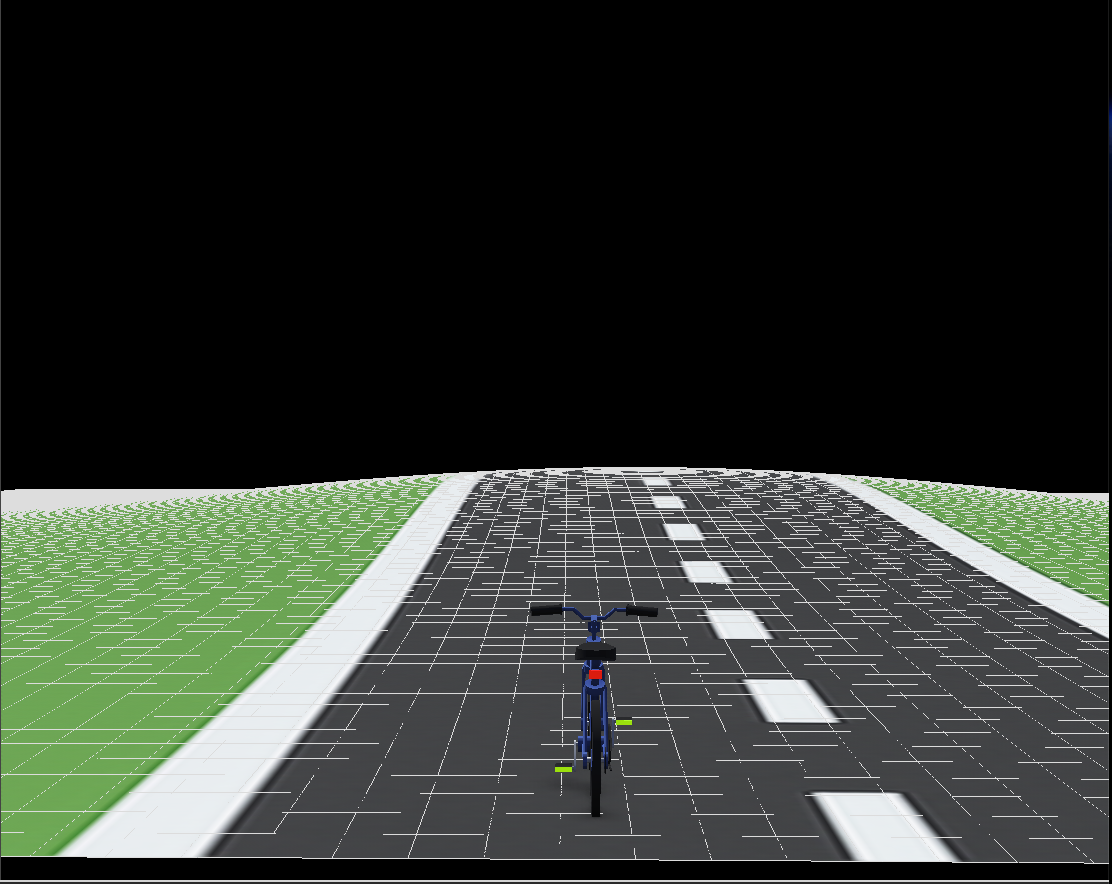
\includegraphics[width=\linewidth]{figures/Huegel.png}
      \caption{Hügel}\label{fig:huegel}
    \end{subfigure}\hfill
    \begin{subfigure}[t]{0.48\textwidth}
      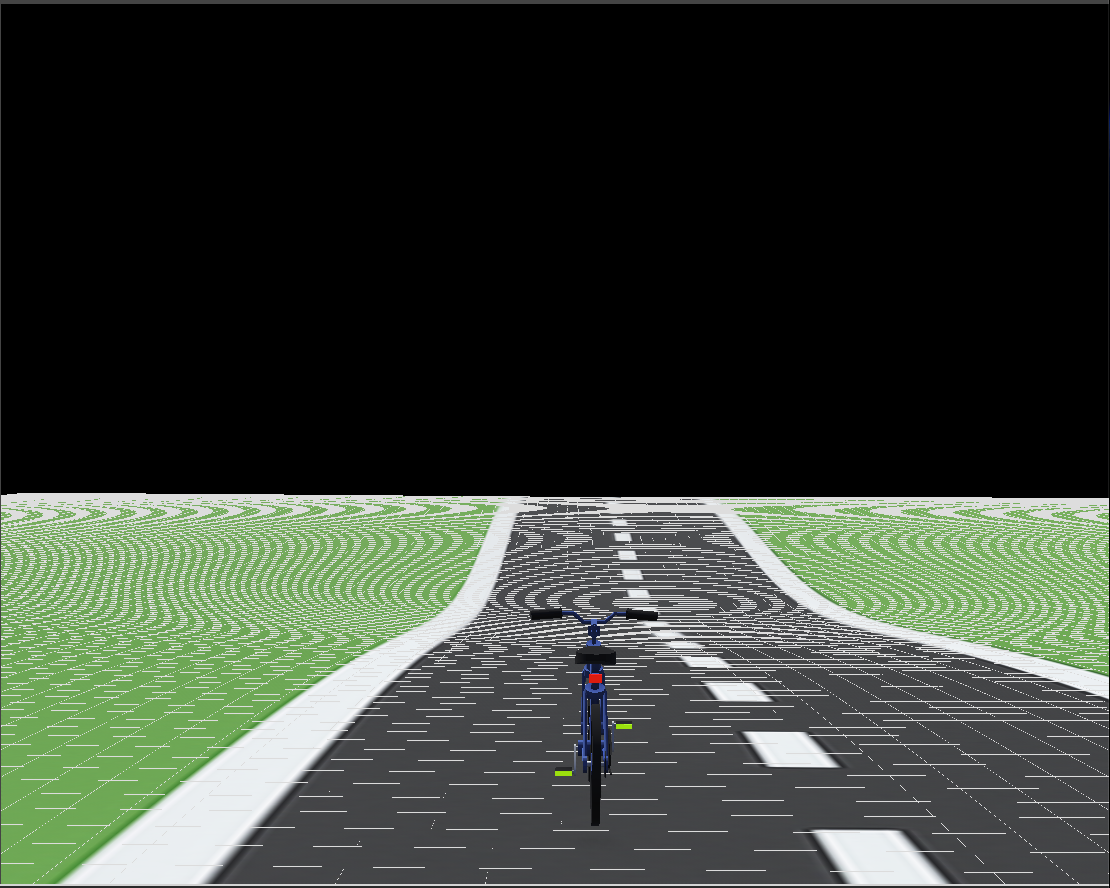
\includegraphics[width=\linewidth]{figures/Tunnel.png}
      \caption{Tunnel}\label{fig:tunnel}
    \end{subfigure}
    \caption{Hügel und Tunnel nebeneinander.}\label{fig:huegel-tunnel}
  \end{figure}
  

  %------------------------------------------------------------------------------------------------
  %------------------------------------------------------------------------------------------------

\subsection{Balance-Stabilität}
\subsection{Spurtreue \& Querabweichung}
\subsection{Rechenzeit \& Echtzeitfähigkeit}
\newpage

%--------------------------------------------------
% Grenzen der Arbeit
%--------------------------------------------------
  \section{Grenzen der Arbeit}

Die vorliegende Arbeit demonstriert die Machbarkeit einer kombinierten Balance- und Spurführungs-Regelung für ein 
selbstbalancierendes Fahrrad in einer Webots-Simulationsumgebung. Trotz der erzielten positiven Ergebnisse weist die entwickelte 
Lösung verschiedene Limitierungen auf, die sowohl methodischer als auch technischer Natur sind. Diese Grenzen sind teilweise 
bewusst gewählte Vereinfachungen zur Fokussierung auf die Kernproblematik, teilweise aber auch ureigene Beschränkungen 
der gewählten Ansätze. Eine transparente Darstellung dieser Limitierungen ist essentiell für die Einordnung der Ergebnisse und 
bildet die Grundlage für zukünftige Erweiterungen des Systems.

\subsection{Simulationsbedingte Limitierungen}

\subsubsection{Inertial Measurement Unit (IMU)}
Die Sensordatenerfassung in der Webots-Simulationsumgebung weist fundamentale 
Unterschiede zur realen Hardware-Implementierung auf, die erhebliche Auswirkungen auf die Übertragbarkeit der entwickelten 
Regelungsalgorithmen haben. Diese Diskrepanz manifestiert sich besonders deutlich beim Vergleich zwischen der verwendeten 
\texttt{InertialUnit} in Webots und dem in den Vorarbeiten eingesetzten BNO055-IMU-Sensor.

Während die Webots-\texttt{InertialUnit} über die API-Funktion \texttt{wb\_inertial\_unit\_get\_roll\_pitch\_yaw()} exakte 
Euler-Winkel ohne jegliche Messfehler bereitstellt, unterliegt der reale BNO055-Sensor einer Vielzahl von Fehlerquellen und 
Hardware-Limitierungen. Die Arbeiten von Ranz (2021) und Karabila (2022) dokumentieren diese Problematik ausführlich und 
zeigen die Komplexität der realen Sensordatenverarbeitung auf.

Der BNO055 arbeitet als 9-Achsen-Fusionssensor, der Accelerometer-, Gyroscope- und Magnetometer-Daten intern verarbeitet und 
über I²C-Kommunikation 16-Bit-Rohwerte ausgibt. Diese müssen über konfigurierbare Skalierungsfaktoren in physikalische Einheiten konvertiert werden \citep{ranz2021bachelor}. Die endliche Auflösung führt zwangsläufig 
zu Quantisierungsfehlern, die bei der hochfrequenten Balance-Regelung (500\,Hz) akkumulieren können. Zusätzlich erfordert der Sensor 
eine mehrstufige Kalibrierung seiner Teilkomponenten, wobei Ranz die Implementierung einer \texttt{set\_axis\_mode()}-Funktion für 
das erforderliche Achsenremapping dokumentiert.

Besonders kritisch erweist sich die Temperaturabhängigkeit des BNO055, die zu zeitvarianten Bias-Fehlern führt. Diese Drift-Effekte 
akkumulieren über die Betriebszeit und können die Regelstabilität beeinträchtigen. Im Gegensatz dazu liefert die Webots-Simulation 
zeitinvariante, temperaturunabhängige Messungen. Die I²C-Kommunikation über \texttt{/dev/i2c-2} auf dem BeagleBone Black verursacht 
zusätzlich variable Kommunikationslatenzen, die Ranz durch spezielle Timeout-Mechanismen und Pufferstrategien kompensieren musste.

Diese Diskrepanzen zwischen Simulation und Realität lassen sich durch verschiedene Ansätze verringern. Die Implementierung eines 
konfigurierbaren Rauschmodells in der Webots-Simulation könnte die spektralen Eigenschaften des BNO055 nachbilden, beispielsweise
durch Überlagerung von weißem Rauschen und charakteristischem 1/f-Rauschen\footnote{1/f-Rauschen, auch als Rosa Rauschen bezeichnet, 
ist ein frequenzabhängiges Rauschsignal, dessen Leistungsdichte proportional zu 1/f abnimmt. Es tritt charakteristisch in 
elektronischen Bauelementen und Sensoren auf und führt zu niederfrequenten Drifteffekten.}. Kommunikationslatenzen ließen sich durch zeitliche 
Pufferung der Sensordaten über mehrere Simulationsschritte simulieren. Systematische Kalibrierungsfehler und temperaturabhängige 
Drift könnten durch langsam variierende Bias-Terme modelliert werden, die von simulierten Umgebungsparametern abhängen.

%--

\subsubsection{Kamera und Vision-Pipeline}
Die Kamerasensorik zeigt analog zur IMU-Problematik erhebliche Unterschiede zwischen der 
idealisierten Webots-Simulation und realen Implementierungen. Diese Diskrepanz wird besonders deutlich bei der Betrachtung von 
Girays (2024) Vision-basierter MPC-Implementierung, die eine YOLOv8-Segmentierung für die Spurerkennung einsetzt.

Die Webots-Kamera erzeugt perfekte, rauschfreie Bilder mit konstanter Beleuchtung und ohne Bewegungsunschärfe oder optische 
Verzerrungen. Girays reale Implementierung auf dem NVIDIA Jetson Nano hingegen musste verschiedene hardware- und umgebungsbedingte 
Herausforderungen bewältigen. Das YOLOv8-Segmentierungsmodell wurde mit einem spezifischen Datensatz für vier Klassen trainiert 
(\textit{meadow}, \textit{obstacle}, \textit{street\_main}, \textit{street\_side}) und mittels TensorRT für die Inferenz optimiert, 
um Bildauswertungszyklen von etwa 100\,ms zu erreichen \citep{vision_mpc_readme}.

Während die Webots-Simulation deterministisch identische Bilder unter kontrollierten Bedingungen liefert, unterliegt die reale 
Kameraverarbeitung verschiedenen Störfaktoren. Girays Implementierung dokumentiert Herausforderungen bei der Echtzeitverarbeitung, 
wobei die Inferenzzeit des YOLOv8-Modells auf eingebetteter Hardware kritisch für die angestrebte 20\,Hz-Abtastrate der Vision-Pipeline 
wird. \pdfcomment{Hier sich sein mit den hz}Die in der Simulation problemlos erreichbare Bildverarbeitung erfordert in der Realität komplexe 
Optimierungsstrategien wie TensorRT-Beschleunigung und Modellkompression.

Die monokulare Kameraarchitektur in Girays System limitiert zusätzlich die Tiefenwahrnehmung auf geometrische Approximationen. Während 
dies in der 2D-Simulation von Webots unproblematisch ist, führt es in realen 3D-Umgebungen zu Unsicherheiten bei der Entfernungsschätzung 
und Hinderniserkennung. Girays Arbeit identifiziert diese Limitation explizit und schlägt stereo-basierte oder LiDAR-gestützte Ansätze für 
zukünftige Implementierungen vor.

Die Übertragung von Girays Vision-Pipeline in die Webots-Simulation abstrahiert von diesen realen Herausforderungen und kann daher zu 
optimistischen Performance-Bewertungen führen. Algorithmen, die in der idealisierten Simulationsumgebung robust funktionieren, können 
unter realen Bedingungen mit variierenden Lichtverhältnissen, Bewegungsunschärfe und Hardwarelimitierungen versagen.

Zusätzlich ist die IPC-Kommunikation zwischen den Controllern in Webots idealisiert und weist keine Paketverluste oder variable Latenzen 
auf. Reale Kommunikationssysteme (UART, Ethernet, CAN) können hingegen variable Latenzen je nach Systemlast, Paketverluste durch 
Übertragungsfehler sowie Jitter durch unregelmäßige Ankunftszeiten der Nachrichten aufweisen. Diese Effekte können die Stabilität 
des Gesamtsystems beeinträchtigen und erfordern robuste Kommunikationsprotokolle mit Fehlerbehandlung und Timeout-Mechanismen.

Die aufgezeigten Unterschiede zwischen idealisierter Simulation und realer Sensorik stellen eine der kritischsten Limitierungen für 
die direkte Übertragbarkeit der entwickelten Regelungsstrategien dar. Sie unterstreichen die Notwendigkeit einer mehrstufigen 
Validierungsstrategie, die von der Simulation über Hardware-in-the-Loop-Tests bis hin zu realen Fahrversuchen reicht.

\subsubsection{Vereinfachte Physikmodellierung}
Wie in Kapitel \ref{sec:ode} dargestellt, basiert die Webots-Simulation auf der Open Dynamics Engine (ODE). Die dort beschriebenen 
Eigenschaften und Implementierungsdetails von ODE führen jedoch zu verschiedenen grundlegenden Limitierungen, die Auswirkungen 
auf die Realitätstreue der Fahrradsimulation haben und die Übertragbarkeit der Ergebnisse auf reale Systeme teilweise einschränken.

Die kritischsten Limitierungen betreffen die vereinfachte Reifen-Fahrbahn-Modellierung und numerische Stabilitätsprobleme. ODE reduziert 
den Reifenkontakt auf eine Punkt-zu-Ebene-Interaktion mit konstantem Reibungskoeffizienten, während reale Reifen komplexe nichtlineare 
Charakteristika aufweisen. Besonders die fehlende Modellierung des Seitenschlupfes, der bei Kurvenfahrten die lateralen Führungskräfte 
bestimmt, beeinträchtigt die Realitätstreue der Fahrdynamik erheblich \citep{catto2009ode_friction}. Im Gegensatz zu den in der 
Fahrzeugdynamik etablierten detaillierten Reifenmodellen \citep{schramm2018fahrzeugdynamik} vernachlässigt die ODE-Simulation 
fundamentale Aspekte der Reifen-Fahrbahn-Interaktion.

Der verwendete explizite Euler-Integrator\footnote{Der Euler-Integrator ist ein numerisches Verfahren zur Lösung von Differentialgleichungen, das aufgrund seiner einfachen Implementierung weit verbreitet ist, jedoch bei großen Zeitschritten oder steifen Systemen zu Stabilitätsproblemen neigt.} kann bei der hochfrequenten Balance-Regelung (500\,Hz) zu numerischen Instabilitäten führen, 
was die Validität der Simulationsergebnisse gefährdet \citep{smith2006ode_stability}. Zusätzlich vernachlässigt die vereinfachte 
Mehrkörperdynamik-Modellierung wichtige Aspekte wie Spiel in Lagern und elastische Verformungen des Rahmens.

Diese fundamentalen Limitierungen der ODE-basierten Physikmodellierung stellen eine erhebliche Einschränkung für die Übertragbarkeit der 
Simulationsergebnisse auf reale Fahrradsysteme dar und erfordern eine kritische Bewertung der erzielten Regelungsperformance.

\textbf{Hardware-Transfer-Implikationen:}

Die Übertragung der ODE-basierten Simulationsergebnisse auf reale Hardware wird zusätzlich durch verschiedene implementierungsspezifische 
Faktoren erschwert. Die Webots-Simulation abstrahiert von vielen hardwarespezifischen Details wie PWM-Charakteristika mit ihren 
Nichtlinearitäten und Totzeiten der Motoransteuerung, mechanischem Spiel in Getrieben und Lagern sowie Temperaturdrift und Verschleiß, 
die das Langzeitverhalten und die Degradation der Komponenten beeinflussen. Diese Faktoren können das reale Systemverhalten erheblich 
von der idealisierten Simulation abweichen lassen und erfordern robuste Adaptationsstrategien bei der Hardware-Implementierung.




%--------------------------------------------------
% Zukünftige Arbeiten (Sensor-Fusion, Reinforcement Learning, Hardware-in-the-Loop)
%--------------------------------------------------
  \section{Zukünftige Arbeiten}

Die vorliegende Arbeit hat ein umfassendes System zur Regelung eines selbstbalancierenden Fahrrads entwickelt, das eine duale Controller-Architektur mit PID-basierter Balance-Regelung und YOLO-gestützter Vision-Kontrolle implementiert. Trotz der erzielten Erfolge in der Simulation zeigen sich mehrere vielversprechende Forschungsrichtungen, die das System erheblich erweitern und verbessern könnten.

\subsection{Sensor-Fusion für robuste Zustandsschätzung}

Das aktuelle System basiert primär auf IMU-Daten zur Roll-Winkel-Bestimmung und Kamerabildern für die Spurerkennung. Eine Integration multipler Sensoren durch fortgeschrittene Sensor-Fusion-Techniken würde die Robustheit und Genauigkeit des Systems erheblich steigern.

\subsubsection{Erweiterte Kalman-Filter-Implementierung}
Die Implementierung eines Extended Kalman Filters (EKF) oder Unscented Kalman Filters (UKF) zur Fusion von IMU-, Kamera- und zusätzlichen Sensordaten stellt eine natürliche Erweiterung dar. Der EKF könnte folgende Sensormodalitäten integrieren:

\begin{itemize}
    \item \textbf{IMU-Fusion}: Kombination von Gyroskop-, Beschleunigungs- und Magnetometer-Daten für präzise Orientierungsschätzung
    \item \textbf{Optischer Fluss}: Ergänzung zur YOLO-Segmentierung für kontinuierliche Bewegungsschätzung
    \item \textbf{Ultraschall/LiDAR}: Abstandsmessung für Hinderniserkennung und 3D-Umgebungsmodellierung
    \item \textbf{Encoder-Fusion}: Integration von Rad- und Lenkwinkel-Encodern für kinematische Konsistenz
\end{itemize}

Die Zustandsschätzung würde dabei den Systemzustand $\mathbf{x} = [x, y, \theta, \dot{x}, \dot{y}, \dot{\theta}, \phi_{roll}, \delta_{steer}]^T$ umfassen, wobei die Prozess- und Messmodelle die nichtlineare Fahrradkinematik berücksichtigen.

\subsubsection{Adaptive Sensor-Gewichtung}
Ein adaptives Gewichtungssystem könnte die Zuverlässigkeit verschiedener Sensoren dynamisch bewerten und entsprechend anpassen. Bei schlechten Lichtverhältnissen würde beispielsweise die Gewichtung der Kameradaten reduziert und die IMU-Daten stärker berücksichtigt.

\subsection{Reinforcement Learning für optimale Regelung}

Während die aktuelle PID-Regelung für grundlegende Stabilisierung ausreicht, bietet Reinforcement Learning (RL) das Potenzial für adaptive und optimale Regelstrategien, die sich an verschiedene Fahrbedingungen anpassen können.

\subsubsection{Deep Deterministic Policy Gradient (DDPG)}
Die Implementierung eines DDPG-Algorithmus würde kontinuierliche Aktionsräume für Lenkwinkel und Geschwindigkeit ermöglichen. Der Zustandsraum könnte erweitert werden um:

\begin{itemize}
    \item Aktuelle und historische Sensordaten (IMU, Kamera, Geschwindigkeit)
    \item Pfadkrümmung und Vorausschau-Informationen
    \item Umgebungsbedingungen (Windstärke, Oberflächenbeschaffenheit)
    \item Systemzustand (Batteriestand, Motortemperatur)
\end{itemize}

Das Belohnungssystem würde Balance-Erhaltung, Spurgenauigkeit und Energieeffizienz optimieren:
\begin{equation}
R_t = w_1 \cdot R_{balance} + w_2 \cdot R_{tracking} + w_3 \cdot R_{energy} + w_4 \cdot R_{safety}
\end{equation}

\subsubsection{Hierarchisches Reinforcement Learning}
Ein hierarchischer Ansatz könnte verschiedene Abstraktionsebenen implementieren:
\begin{itemize}
    \item \textbf{High-Level Policy}: Pfadplanung und Geschwindigkeitsstrategie
    \item \textbf{Mid-Level Policy}: Kurvenstrategie und Hindernisumfahrung  
    \item \textbf{Low-Level Policy}: Direkte Motor-Ansteuerung für Balance
\end{itemize}

\subsubsection{Transfer Learning und Sim-to-Real}
Die Übertragung der in Webots trainierten RL-Modelle auf reale Hardware erfordert Domain Adaptation-Techniken. Ansätze wie Domain Randomization während des Trainings und progressive Realitätsanpassung könnten die Sim-to-Real-Lücke überbrücken.

\subsection{Hardware-in-the-Loop für realitätsnahe Validierung}

Die Validierung des entwickelten Systems erfordert eine schrittweise Annäherung an reale Bedingungen durch Hardware-in-the-Loop (HIL) Simulationen.

\subsubsection{Embedded Controller Integration}
Die Portierung der C-basierten Balance-Regelung auf Embedded-Systeme wie BeagleBone Black oder Raspberry Pi würde realistische Rechenzeit- und Ressourcenbeschränkungen einführen. Kritische Aspekte umfassen:

\begin{itemize}
    \item \textbf{Real-Time Constraints}: Garantierte Ausführungszeiten für die 500Hz Balance-Regelschleife
    \item \textbf{Interrupt-Handling}: Prioritätsbasierte Behandlung von Sensor-Interrupts
    \item \textbf{Memory Management}: Optimierte Datenstrukturen für begrenzte RAM-Ressourcen
    \item \textbf{Power Management}: Energieeffiziente Algorithmen für Batteriebetrieb
\end{itemize}

\subsubsection{Sensorik-Hardware-Integration}
Die Integration realer Sensoren würde Rauschen, Latenz und Ausfälle einführen:
\begin{itemize}
    \item \textbf{IMU-Kalibrierung}: Bias-Kompensation und Temperaturkorrekturen
    \item \textbf{Kamera-Latenz}: Bildverarbeitungs-Pipeline mit ~50ms Verzögerung
    \item \textbf{Sensor-Ausfälle}: Graceful Degradation bei Sensor-Fehlern
\end{itemize}

\subsubsection{Aktorik-Hardware-Modellierung}
Realistische Motormodelle würden Trägheit, Backlash und Sättigungseffekte berücksichtigen:
\begin{equation}
\tau_{motor} = K_t \cdot i_{motor} - B \cdot \omega_{motor} - \tau_{friction}(\omega_{motor})
\end{equation}

\subsection{Systemintegration und Validierung}

\subsubsection{Modular Testing Framework}
Ein systematisches Test-Framework würde verschiedene Komplexitätsstufen ermöglichen:
\begin{enumerate}
    \item \textbf{Unit Tests}: Einzelne Algorithmus-Komponenten
    \item \textbf{Integration Tests}: Sensor-Fusion und Controller-Interaktion  
    \item \textbf{System Tests}: Vollständige HIL-Simulation
    \item \textbf{Field Tests}: Reale Hardware-Validierung
\end{enumerate}

\subsubsection{Performance Metriken}
Quantitative Bewertungskriterien würden umfassen:
\begin{itemize}
    \item \textbf{Balance-Performance}: RMS Roll-Winkel, Zeit bis zum Umfallen
    \item \textbf{Tracking-Genauigkeit}: Laterale Abweichung, Pfadverfolgungsfehler
    \item \textbf{Energieeffizienz}: Verbrauch pro Kilometer, Regenerationsrate
    \item \textbf{Robustheit}: Performance unter Störungen und Sensorausfällen
\end{itemize}

\subsection{Fazit und Ausblick}

Die vorgeschlagenen Erweiterungen würden das selbstbalancierende Fahrrad von einem Simulationsprototyp zu einem robusten, adaptiven System entwickeln. Die Kombination aus fortgeschrittener Sensor-Fusion, lernfähigen Regelungsalgorithmen und realitätsnaher Hardware-Integration stellt eine natürliche Evolution des aktuellen Ansatzes dar. 

Besonders vielversprechend ist die Möglichkeit, durch Reinforcement Learning nicht nur die Regelungsperformance zu optimieren, sondern auch neue Fahrstrategien zu entdecken, die über klassische Regelungsansätze hinausgehen. Die systematische HIL-Validierung würde dabei sicherstellen, dass die entwickelten Algorithmen auch unter realen Bedingungen zuverlässig funktionieren.

Diese Forschungsrichtungen adressieren sowohl die technischen Herausforderungen der Systemrealisierung als auch die wissenschaftlichen Fragen der optimalen Regelung komplexer, unteraktuierter Systeme und tragen somit zur Weiterentwicklung autonomer Fahrzeugsysteme bei.

%--------------------------------------------------
% Fazit
%--------------------------------------------------
  \section{Fazit}

Diese Masterarbeit hat erfolgreich eine zweistufige Regelungsarchitektur für ein selbstbalancierendes Fahrrad entwickelt und in der 
Webots-Simulationsumgebung validiert. Die systematische Integration einer hochfrequenten PID-Balanceregelung (500\,Hz) mit einer
 visionbasierten MPC-Spurführung (20\,Hz) stellt einen wichtigen methodischen Fortschritt in der Entwicklung autonomer Fahrradsysteme dar.

\subsection{Zentrale Erkenntnisse}

Die entwickelte duale Controller-Architektur demonstriert erstmals die praktische Machbarkeit der Kopplung von 
Balance- und Fahrtrichtungsregelung in einer integrierten Simulationsumgebung. Die erfolgreiche Portierung 
bewährter Hardware-Implementierungen von Zander (2023) und Giray (2024) zeigt die Übertragbarkeit etablierter 
Regelungskonzepte zwischen verschiedenen Plattformen auf.

Ein überraschendes und bedeutsames Ergebnis ist die durchgängige Überlegenheit der ROI-basierten Fallback-Erkennung 
gegenüber der YOLO-Segmentierung. In allen Testszenarien erwies sich die klassische Bildverarbeitung als überlegen: 
Bei der Kurvenfahrt erreichte ROI-Fallback 43,62\,s stabile Fahrt gegenüber 35,96\,s bei YOLO-PID, in der S-Kurve 
ergab sich eine 16,8\% Verbesserung der Fahrtdauer mit halbierten Querfehlern. Diese Ergebnisse zeigen, dass für 
strukturierte Simulationsumgebungen klassische Bildverarbeitung durchaus konkurrenzfähig zu modernen 
Deep-Learning-Ansätzen sein kann.

Die systematische Evaluierung verschiedener Störungsszenarien belegt die Anpassungsfähigkeit der 
Regelungsarchitektur. Das System bewältigt Seitenwind bis 1,0\,m/s und Höhenunterschiede bis 4\,m 
durch adaptive PID-Parametrierung, wobei sich Senken als weniger kritisch als Hügel erweisen.

\subsection{Methodische Beiträge}

Die Arbeit etabliert eine systematische Methodik für die risikofreie Entwicklung und Validierung 
komplexer Regelungsstrategien in Webots. Das entwickelte JSON-basierte Konfigurationssystem mit 
grafischem Interface unterstützt iteratives Parameter-Tuning, während die hochfrequente Datenerfassung 
(2\,ms Abtastung) detaillierte Regeldynamik-Analysen ermöglicht.

\subsection{Limitierungen und kritische Reflexion}

Die identifizierten Grenzen ordnen die Ergebnisse in einen realistischen wissenschaftlichen Kontext ein. 
Besonders kritisch für eine praktische Umsetzung erweisen sich die sensorischen Idealisierungen (perfekte IMU- 
und Kameradaten ohne Rauschen oder Drift), die vereinfachte ODE-basierte Physikmodellierung und die 
Echtzeitfähigkeits-Herausforderungen bei der Vision-Pipeline auf eingebetteten Systemen.

Die Hardware-Transfer-Problematik manifestiert sich auf mehreren Ebenen: von der numerischen Stabilität der 
Physiksimulation über Kommunikationslatenzen bis hin zu mechanischen Toleranzen und elektronischen Nichtlinearitäten, 
die in der Simulation vollständig abstrahiert werden.

\subsection{Wissenschaftlicher Beitrag}

Diese Arbeit leistet vier wesentliche Beiträge zur Forschung: (1) die erstmalige erfolgreiche Integration von 
Balance- und Spurführungsregelung, (2) systematische Methodenvergleiche zwischen verschiedenen Ansätzen, (3) 
umfassende Robustheitsvalidierung unter verschiedenen Störungsszenarien und (4) die Entwicklung einer modularen, 
erweiterbaren Regelungsarchitektur.

\subsection{Ausblick}

Methodisch unterstreichen die aufgezeigten Grenzen die Notwendigkeit einer mehrstufigen Validierungsstrategie, 
die von der Simulation über Hardware-in-the-Loop-Tests bis hin zu systematischen Feldversuchen reicht. Zukünftige 
Forschungsrichtungen sollten sich auf die systematische Überbrückung der Sim-to-Real-Lücke konzentrieren, 
insbesondere durch Integration hardware-spezifischer Charakteristika, erweiterte Physikmodellierung und 
Multi-Environment-Training.

Trotz der identifizierten Limitierungen bildet die vorliegende Arbeit eine fundierte Grundlage für die 
Weiterentwicklung autonomer selbstbalancierender Fahrradsysteme. Die erfolgreiche Demonstration der 
kombinierten Regelungsarchitektur und die detaillierte Dokumentation der Systemgrenzen schaffen eine 
solide Basis für zukünftige Forschungsarbeiten und unterstreichen die Bedeutung einer kritischen Reflexion 
der Übertragbarkeit von Simulationsergebnissen auf reale Anwendungen.
%--------------------------------------------------
% Literaturverzeichnis
%--------------------------------------------------
\section{Literaturverzeichnis}
% Hier später \bibliographystyle und \bibliography einfügen
%--------------------------------------------------
% Anhang (Parametertabellen, Screenshots, Release-Link)
%--------------------------------------------------
\newpage
\bibliography{refs}
\end{document}

